\documentclass[areasetadvanced]{scrartcl}

\usepackage[utf8]{inputenc}
\usepackage[T2A]{fontenc}
\usepackage[english,russian]{babel}
\usepackage{xcolor}

\usepackage[footskip=1cm,left=25mm, right=15mm, top=20mm, bottom=20mm]{geometry}
\usepackage{setspace}
\usepackage{amsmath, amssymb} 
\usepackage{graphicx}
\usepackage{tikz}
\usetikzlibrary{arrows.meta}
\usepackage{float}
\usepackage{dashrule}
\usepackage{fancyhdr} 
\usepackage{hyperref} 
\usepackage{parskip}
\usepackage{textcomp, enumitem}
\usepackage{indentfirst}
\usepackage{graphicx}
\usepackage{algorithm}
\usepackage{xltabular}
\usepackage{xtab}
\usepackage{algpseudocode}
\usepackage{array} 
\usepackage{geometry}
\usepackage{afterpage}
\usepackage{minted}
\setcounter{secnumdepth}{3} 
\setcounter{tocdepth}{3}    
\usepackage{listings} 
\usepackage{booktabs}
\usepackage{paracol} % параллельные колонки (левая/правая)

\newcommand{\icon}[1]{\includegraphics[height=1.2em]{#1}}

\tikzstyle{block} = [rectangle, rounded corners, minimum width=3cm, minimum height=1cm, text centered, draw=black, fill=lightgray]

\setkomafont{sectioning}{\normalfont\bfseries} 
\setkomafont{section}{\normalfont\Large\bfseries}
\setkomafont{subsection}{\normalfont\large\bfseries}
\setkomafont{subsubsection}{\normalfont\large\bfseries}
\setkomafont{paragraph}{\normalfont\large\bfseries} 
\newcommand{\twosideheading}[2]{%
  \noindent
  \begin{minipage}[t]{0.5\textwidth}\raggedright\small #1\end{minipage}%
  \begin{minipage}[t]{0.5\textwidth}\raggedleft\Large\bfseries #2\end{minipage}\\[-0.2em]
  \hrule
  \vspace{0.8em}
}
\lstset{
  language=Haskell,
  basicstyle=\ttfamily\small,
  keywordstyle=\color{blue}\bfseries,
  stringstyle=\color{red},
  commentstyle=\color{green!70!black},
  numbers=left,
  numberstyle=\tiny,
  stepnumber=1,
  numbersep=10pt,
  showstringspaces=false,
  breaklines=true,
  frame=single
}

\lstdefinelanguage{Lua}{
    keywords={function, end, if, then, else, elseif, for, while, do, repeat, until, break, return, local, and, or, not, true, false, nil},
    keywordstyle=\color{blue}\bfseries,
    stringstyle=\color{red},
    commentstyle=\color{green!70!black},
    morestring=[s]{"}{"},
    morestring=[s]{'}{'},
    morecomment=[l]{-},
    morecomment=[s]{-[[}{]]},
    basicstyle=\ttfamily\small,
    numbers=left,
    numberstyle=\tiny,
    stepnumber=1,
    numbersep=10pt,
    showstringspaces=false,
    breaklines=true,
    frame=single
}

\lstdefinestyle{py}{
    language=Python,
    basicstyle=\ttfamily\small,
    keywordstyle=\color{blue}\bfseries,
    stringstyle=\color{red},
    commentstyle=\color{green!70!black},
    numbers=left,
    numberstyle=\tiny,
    stepnumber=1,
    numbersep=10pt,
    showstringspaces=false,
    breaklines=true,
    frame=single
}

\setlength{\parindent}{1.25cm}
\setcounter{tocdepth}{3}
\begin{document}
\sloppy
	\thispagestyle{empty}
	\begin{center}
		\large{МИНОБРНАУКИ РОССИИ} \par
		\vspace{0.3cm}
		\normalsize
		{ФЕДЕРАЛЬНОЕ ГОСУДАРСТВЕННОЕ АВТОНОМНОЕ ОБРАЗОВАТЕЛЬНОЕ УЧРЕЖДЕНИЕ ВЫСШЕГО ОБРАЗОВАНИЯ} \par
		\vspace{0.3cm}
		\textbf{САНКТ-ПЕТЕРБУРГСКИЙ ПОЛИТЕХНИЧЕСКИЙ}
		\textbf{УНИВЕРСИТЕТ ПЕТРА ВЕЛИКОГО} \par
		\vspace{0.3cm}
		{Институт компьютерных наук и кибербезопасности}\par
		{Высшая школа технологий искусственного интеллекта}\par
	\end{center}
	\vfill
	\begin{center}
		{\huge Отчёт о выполнении лабораторных работ}\par
		%\vspace{0.1cm}
        \huge {по дисциплине:}\par
        \vspace{0.3cm}
		\Huge \textbf{Защита информации}\par
	\end{center}
	\vfill
	\begin{flushleft}
		Студент: \hspace{1.8cm} \rule[0pt]{2.5cm}{0.5pt}\hfill Салимли Айзек Мухтар Оглы\par
		\vspace{1.5cm}
		Преподаватель: \hspace{0.55cm} \rule[0pt]{2.5cm}{0.5pt}\hfill  Силиненко Александр Витальевич
	\end{flushleft}
	\vspace{0.5cm}
	\begin{flushright}
		\guillemotleft \rule[0pt]{0.8cm}{0.5pt}\guillemotright \rule[0pt]{2cm}{0.5pt} 20\rule[0pt]{0.5cm}{0.5pt} г.
	\end{flushright}
	\vfill
	\begin{center}
		Санкт-Петербург, 2026
	\end{center}

\newpage
\begin{center}
	\textbf{РЕФЕРАТ}\par
    \textbf{Объем отчета: N с., M табл., K источн., L прил.}
\end{center}


\textbf{Ключевые слова:} Защита информации, банк угроз, базовые вектора уязвимостей, $\dots$

Отчет содержит информацию о проделанной работе по дисциплине «защита информации», которая включала в себя N лабораторных работ.

\begin{itemize}
    \item \textbf{Практическая работа №1} — Банк угроз ФСТЭК: изучение структуры разделов «Угрозы» и «Уязвимости», поиск уязвимостей по заданным критериям.
    \item \textbf{Практическая работа №2} — Аутентификация и авторизация: разработка системы доступа к конфиденциальным данным, утилиты управления учётными записями и программы brute force для исследования стойкости паролей.
    \item \textbf{Практическая работа №3} — DAC и MAC: реализация дискреционной и мандатной моделей доступа на базе системы аутентификации из работы №2 (владение, ACL, метки безопасности, модель Белла-Лападулы).
    \item $\dots$
\end{itemize}

\newpage

\section*{Термины и определения}
\addcontentsline{toc}{section}{Термины и определения}

В отчете применяют следующие термины с соответствующими определениями:

\begin{center}
\renewcommand{\arraystretch}{0.75}
\setlength{\tabcolsep}{3pt}
\begin{longtable}{>{\raggedright\arraybackslash}p{3.5cm}>{\raggedright\arraybackslash}p{9.5cm}}
\caption{Термины и определения} \\
\label{tab:terms} \\
\toprule
\textbf{Термин} & \textbf{Определение} \\
\midrule
\endfirsthead
\caption[]{Термины и определения (продолжение)} \\
\toprule
\textbf{Термин} & \textbf{Определение} \\
\midrule
\endhead
\midrule
\multicolumn{2}{r}{Продолжение на следующей странице} \\
\endfoot
\bottomrule
\endlastfoot
Информация & Сведения о лицах, предметах, фактах, событиях, явлениях и процессах независимо от формы их представления. \\
\hline
Свойства Безопасности информации &  Конфиденциальность, Целостность, Доступность. \\
\hline
Угроза & Потенциально возможное событие, действие или фактор (внешний или внутренний), способный нарушить конфиденциальность, целостность или доступность данных, нанеся ущерб информационным системам или пользователям. \\
\hline
Риск & Критерий угрозы - вероятность реализации угрозы, использующей уязвимости информационных активов, что приводит к ущербу: нарушению конфиденциальности, целостности или доступности данных. \\
\hline
Банк угроз & официальный общедоступный ресурс, содержащий систематизированный перечень уязвимостей, угроз, способов их реализации и объектов воздействия в информационных системах\cite{bdu}. \\
\hline
ФСТЭК & Федеральная служба по техническому и экспортному контролю. \\
\hline
Программное обеспечение & Совокупность программ, процедур, правил, документации и данных, необходимых для функционирования систем обработки информации. \\
\hline
Операционная система & Совокупность программ, обеспечивающих управление ресурсами ЭВМ и взаимодействие пользователя с машиной. \\
\hline
CWE (Common Weakness Enumeration) & Международная система классификации недостатков, дефектов и уязвимостей в программном и аппаратном обеспечении \\
\hline
Наличие эксплойта & Специальная программа, фрагмент кода или последовательность команд, использующие уязвимости (ошибки, слабые места) в программном обеспечении (ПО) или операционных системах для проведения атаки.\\
\hline
CVSS 2.0 (Common Vulnerability Scoring System, v2.0) & Вторая версия открытого стандарта для оценки серьезности уязвимостей IT-систем \\
\hline
CVSS 3.0 (Common Vulnerability Scoring System, v3.0) & Третья версия открытого стандарта для оценки серьезности уязвимостей IT-систем \\
\hline
Аутентификация & Процесс установления подлинности пользователя или устройства с помощью пароля, ключа или другого идентификатора. \\
\hline
Авторизация & Процесс установления доступа пользователя к ресурсам системы с помощью аутентификации. \\
\hline
Хэширование & Процесс преобразования данных в хеш-значение. \\
\hline
Слабый пароль & Пароль, который легко угадать или подобрать. \\
\hline
Дискреционная модель & Модель, в которой доступ к ресурсам определяется правами пользователя. \\
\hline
Мандатная модель & Модель, в которой доступ к ресурсам определяется уровнем доступа пользователя. \\
\hline
Уровень доступа & Уровень, определяющий права пользователя на доступ к ресурсам системы. \\
\hline
Уровень конфиденциальности & Уровень, определяющий степень секретности информации. \\
\hline
MAC & Mondatory Access Control. \\
\hline
DAC & Discretionary Access Control.
\end{longtable}
\end{center}

\newpage
\tableofcontents

\newpage
\section*{Введение}
\addcontentsline{toc}{section}{Введение}

Защита информации представляет собой совокупность мер, направленных на обеспечение трёх основных свойств информационных систем: конфиденциальности (ограничение доступа к данным только для субъектов, имеющих соответствующие права), целостности (сохранение данных в неизменном виде и защита от несанкционированной модификации) и доступности (обеспечение возможности использования информации и ресурсов для уполномоченных пользователей при необходимости). В настоящем отчёте рассматриваются и реализуются методы и механизмы, позволяющие достичь указанных свойств в практике построения защищённых систем.

Отчет содержит информацию о проделанной работе по дисциплине «Защита информации», которая включала в себя N лабораторных работ.

В практической работе №1 был изучен Банк данных угроз безопасности информации ФСТЭК РФ. Изучена структура раздела \guillemetleft Угрозы\guillemetright и раздела \guillemetleft Уязвимости\guillemetright Банка угроз. Выполнен поиск уязвимостей по заданным критериям для операционной системы ноутбука (macOS) и смартфона (iOS). Проанализированы базовые векторы CVSS у найденных уязвимостей и описаны меры для их устранения.

В практической работе №2 разработана система доступа пользователей к конфиденциальным данным: выделен каталог для хранения файлов, реализована утилита управления учётными данными (пароли, права доступа), утилита доступа к конфиденциальным данным с аутентификацией и авторизацией. Разработана программа взлома паролей методом грубой силы (brute force) и исследована стойкость паролей в зависимости от длины и алгоритма хэширования SHA256.

В практической работе №3 на базе системы аутентификации из работы №2 реализованы модели дискреционного (DAC) и мандатного (MAC) управления доступом. Для DAC: владение объектами, произвольное назначение прав через команды grant/revoke, контроль на основе списка доступа (ACL). Для MAC: метки безопасности для субъектов и объектов (несекретно, ДСП, секретно), свойства модели Белла-Лападулы (\guillemetleft нет чтения сверху\guillemetright, \guillemetleft нет записи вниз\guillemetright).

\newpage
\section{Анализ уязвимостей программного обеспечения}
\subsection{Введение}

Анализ уязвимостей программного обеспечение (далее ПО) - процесс по выявлению недостатков ПО, которые могут
привести к нарушению безопасности информационной системы (см. Таб. \ref{tab:terms}).

Уязвимость представляет собой \guillemetleft  слабое\guillemetright место в ПО, позволяющее злоумышленнику осуществить несанкционированный доступ, атаку или получить контроль над информацией.
Анализ уязвимостей направлен на предотвращение потенциальных угроз и устранение существующих проблем безопасности.

Целью лабораторной работы №1 - является получение навыков работы с банком угроз Федеральной службы по техническому и экспортному контролю (ФСТЭК России).

Банк угроз\cite{bdu} содержит информацию об уязвимостях ПО и методах их эксплуатации. В рамках работы необходимо изучить структуру Банка угроз 
и освоить поиск уязвимостей, для собственной операционной системы компьютера и операционной системы смартфона. 

\subsection{Раздел \guillemetleft  Угрозы\guillemetright}

Раздел \guillemetleft  Угрозы\guillemetright\cite{bdu} содержит информацию об аспектах, связанных с угрозами безопасности информации.
В нем представлена классификация угроз по их природе, воздействию и потенциальным последствиям.
Каждая угроза сопровождается подробным описанием методов атаки, целей и уязвимостей, используемых злоумышленниками.
Для оценки степени серьезности воздействия предусмотрен параметр уровня опасности.
Также раздел включает рекомендации по защите, позволяющие определить меры для предотвращения или минимизации угрозы\cite{bdu}.

В разделе можно фильтровать данные по: 
\begin{itemize}
    \item Контекстному поиску;
    \item По источнику угрозы;
    \item Последствиям реализации угрозы которые включают в себя пункты: \begin{itemize}
        \item Нарушение конфиденциальности;
        \item Нарушение целостности;
        \item Нарушение доступности.
    \end{itemize}
\end{itemize}

Ниже на рисунке \ref{fig:razdel_ugrozi}, представлен снимок экрана, раздела угроз:

\begin{figure}[H]
    \centering
    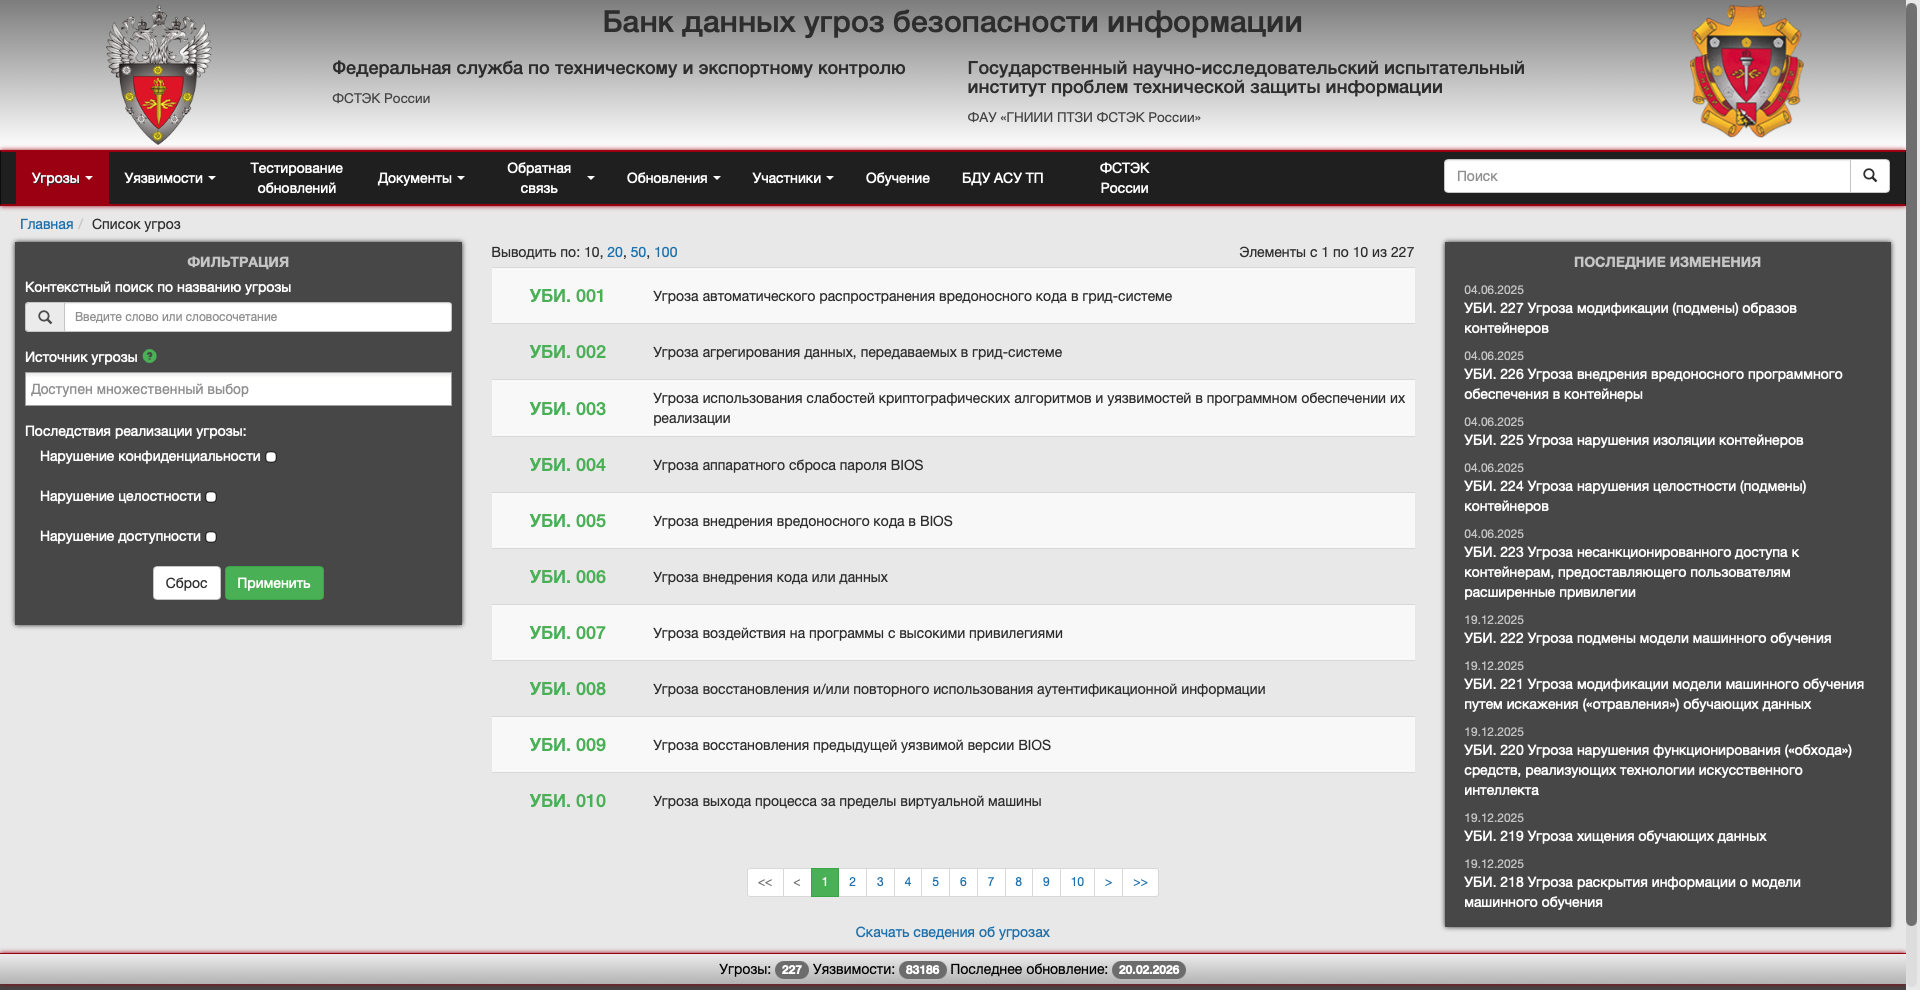
\includegraphics[width=0.60\linewidth]{img/lab-1/RAZDEL_UGROZ.png}
    \caption{Раздел угроз}
    \label{fig:razdel_ugrozi}
\end{figure}

\subsection{Раздел \guillemetleft  Уязвимости\guillemetright}

Раздел \guillemetleft  Список уязвимостей\guillemetright\cite{bdu}, представляет перечень потенциальных недостатков или уязвимых точек в ПО, аппаратуре или в информационных системах
которые могут быть использованы злоумышленниками для нарушения свойств безопасности информации (см. Таб. \ref{tab:terms}).

Основным отличием уязвимости и угрозы - в том, что уязвимость это недостаток ПО (или системы), а угроза - это риск того что уязвимостью воспользуются.

То есть уязвимость существует сама по себе, а угроза существует условно.

Уязвимости делятся по определенным критериям:
\begin{itemize}
    \item Классификация уязвимости - отнесение уязвимости к конкретному классу, например в ФСТЭК классы делятся на: уязвимость кода, уязвимость арихтектуры и многофакторная;
    \item Год добавления - дата, когда уязвимасть была найдена и добавлена в банк угроз;
    \item Уровень опасности - делиться на 4 типа: Низкий, Средний, Высокий, Критический;
    \item Идентификатор типа ошибки - идентификатор, установленный в соответствии с общим перечнем ошибок CWE (см. Таб. \ref{tab:terms});
    \item Наличие эксплойта (см. Таб. \ref{tab:terms}) - Может существовать, быть в открытом доступе, не быть или уточняться;
    \item Способ эксплуатаци - какую именно угрозу несет уязвимость (например SQL-инъекция);
    \item Способ устранения - может быть обновление ПО или организационные меры;
    \item Операционная система - операционная система, под управлением которой функционирует программное обеспечение с обнаруженной уязвимостью.
\end{itemize} 

Наиболее опасная уязвимость - в ФСТЭК является возможность злоумышленника выполнять произвольные команды. 

Это можно увидеть, воспользовавшись сортировкой угроз (см. Рис. \ref{fig:SORT_BY_CRITICAL}) по уровню опасности (по критичности) описаной ранее:

\begin{figure}[H]
    \centering
    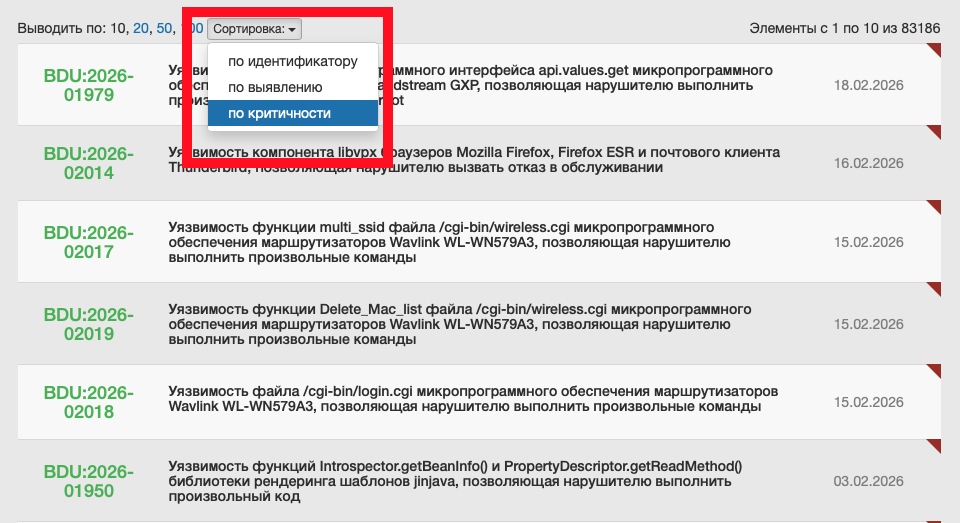
\includegraphics[width=0.60\linewidth]{img/lab-1/SORT_BY_CRITICAL.png}
    \caption{Раздел угроз}
    \label{fig:SORT_BY_CRITICAL}
\end{figure}

Для визуального восприятия уязвимости так же помечаются цветом в соответствии с уровнем опасности:

\begin{itemize}
    \item \textcolor{green}{Низкий уровень опасности}
    \item \textcolor{yellow}{Средний уровень опасности}
    \item \textcolor{orange}{Высокий уровень опасности}
    \item \textcolor{red}{Критический уровень опасности}
\end{itemize}

Так же в разделе \guillemetleft  Уязвимости\guillemetright, есть подраздел \guillemetleft  Инфографика\guillemetright, 
который позволяет визуально оценить следующие данные\cite{bdu}:
\begin{itemize}
    \item Количество критических уязвимостей в ПО различных производителей (см. Рис \ref{fig:info_first})
    \item Распределение уязвимостей по уровням опасности (см. Рис \ref{fig:info_sec})
    \item Распределение уязвимостей по типам ПО (см. Рис \ref{fig:info_third})
    \item Количество уязвимостей в ПО различных производителей (см. Рис \ref{fig:info_fourth})
    \item Распределение уязвимостей по типам ошибок (см. Рис \ref{fig:info_fiveth})
    \item Количество уязвимостей программного обеспечения различных производителей, связанных с инцидентами информационной безопасности (см. Рис \ref{fig:info_sixth})
\end{itemize}

Ниже перечислены все инфографики описанные выше:

\begin{figure}[H]
    \centering
    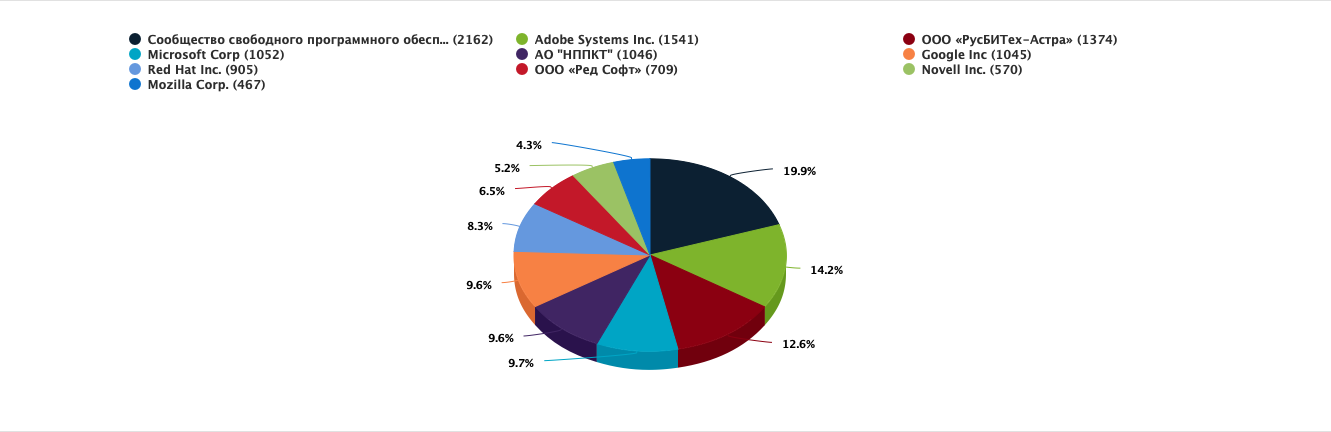
\includegraphics[width=0.60\linewidth]{img/lab-1/info1.png}
    \caption{Количество критических уязвимостей в ПО различных производителей}
    \label{fig:info_first}
\end{figure}

Как видно из гистограммы \ref{fig:info_first}, количество критических уязвимостей больше наблюдается у сообщества 
свободного программного обеспечения. Вероятно это связано с тем, что это не большие компании, где нет отдельных специалистов обеспечивающих должную защиту информации.

\begin{figure}[H]
    \centering
    
\includegraphics[width=0.60\linewidth]{img/lab-1/info2.png}
    \caption{Распределение уязвимостей по уровням опасности}
    \label{fig:info_sec}
\end{figure}

Из рисунка \ref{fig:info_sec}, видно что больше всего уязвимостей имеют средний уровень опасности.

\begin{figure}[H]
    \centering
    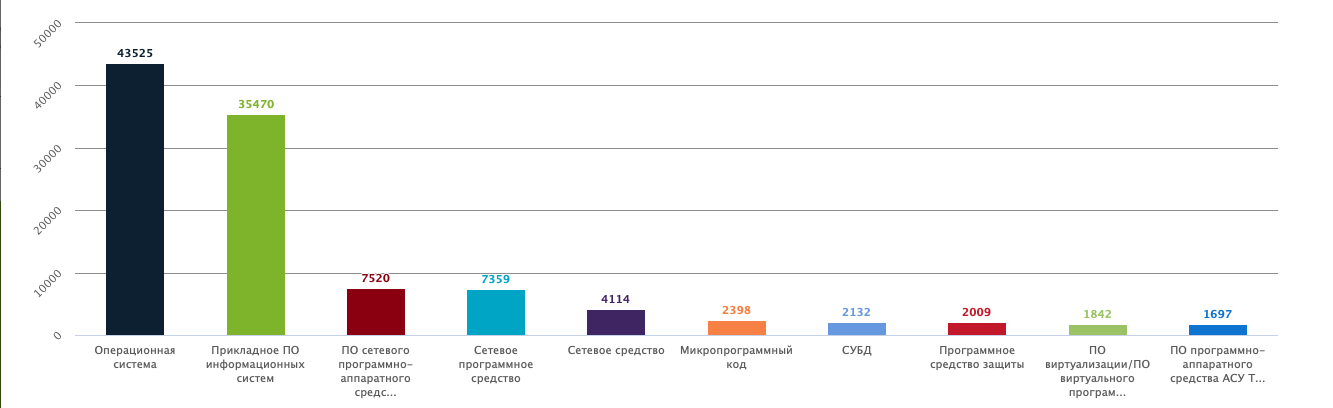
\includegraphics[width=0.60\linewidth]{img/lab-1/info3.png}
    \caption{Распределение уязвимостей по типам ПО}
    \label{fig:info_third}
\end{figure}

Наиболее уязвимый тип ПО - является операционная система (см. Рис. \ref{fig:info_third}), что обусловлено тем, что ОС - довольно объемное и сложно программное обеспечение.

\begin{figure}[H]
    \centering
    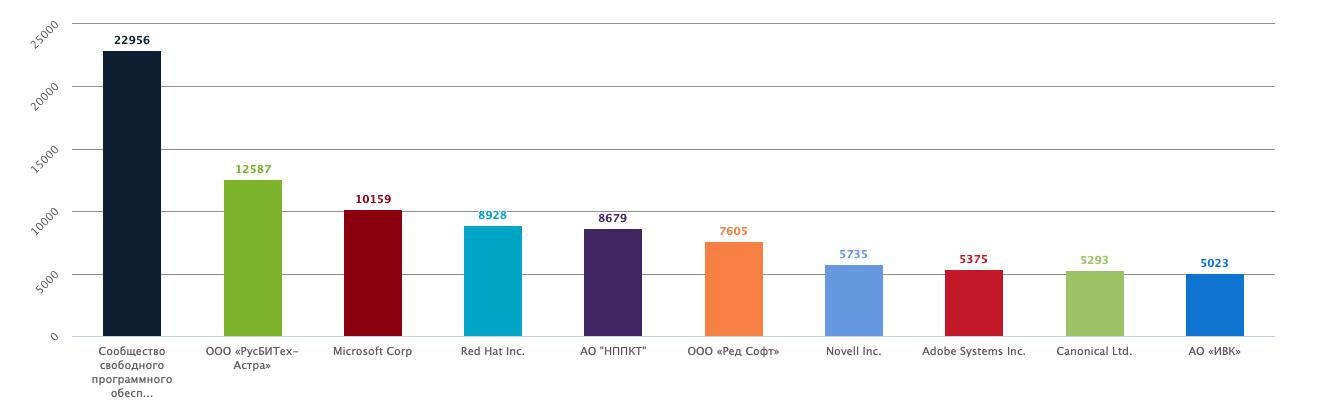
\includegraphics[width=0.60\linewidth]{img/lab-1/info4.png}
    \caption{Количество уязвимостей в ПО различных производителей}
    \label{fig:info_fourth}
\end{figure}

Так же как и в случае с критическими уязвимостями (см. Рис. \ref{fig:info_first}), общее количество уязвимостей больше у сообщества свободного программного обеспечение (см. Рис. \ref{fig:info_fourth}).

\begin{figure}[H]
    \centering
    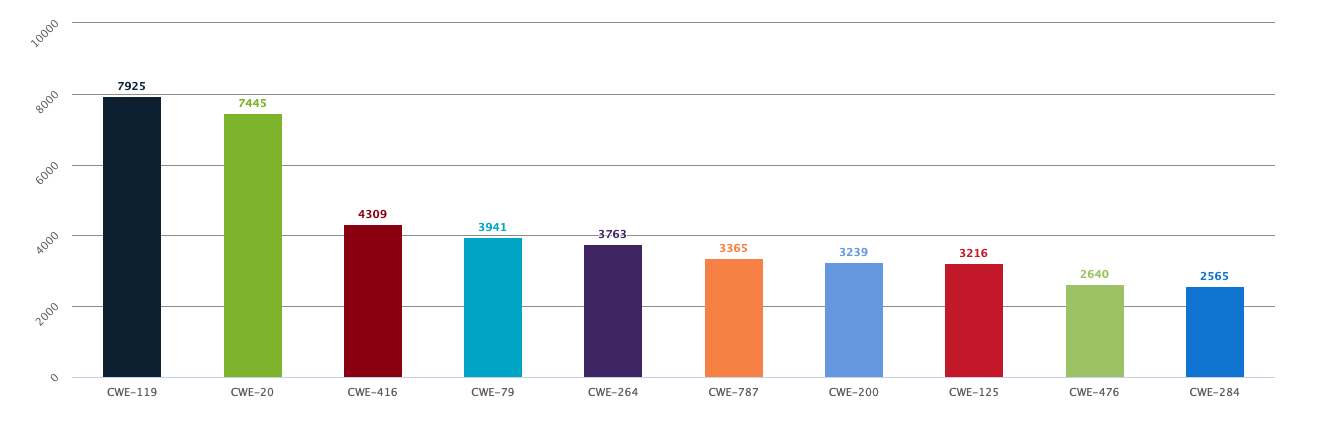
\includegraphics[width=0.60\linewidth]{img/lab-1/info5.png}
    \caption{Распределение уязвимостей по типам ошибок}
    \label{fig:info_fiveth}
\end{figure}

Наиболее частая уязвимость по типу ошибки - CWE-119 (см. Рис. \ref{fig:info_fiveth}). CWE-119 - это ошибка связанная с неправильным ограничением операций в границах буфера памяти.

\begin{figure}[H]
    \centering
    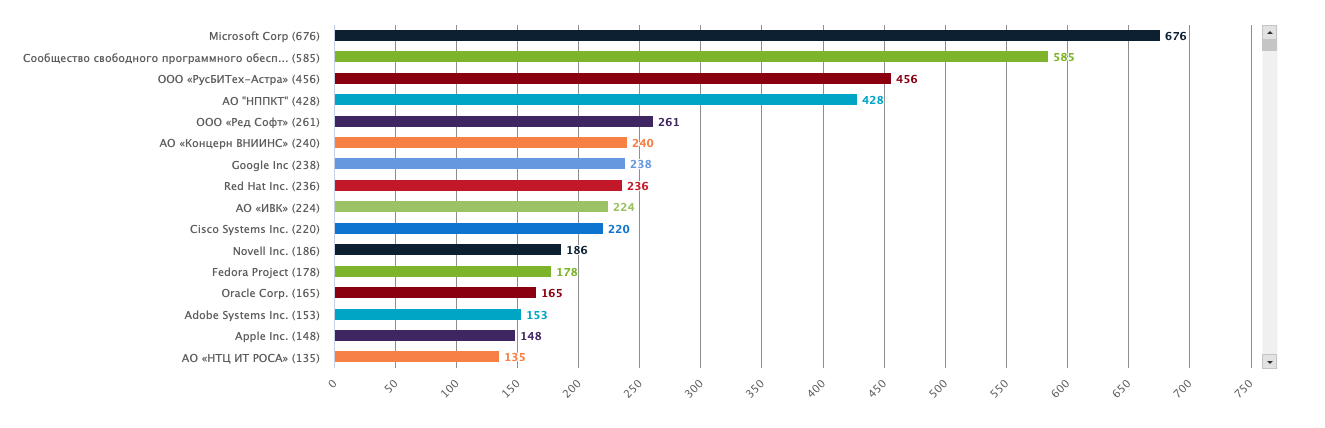
\includegraphics[width=0.60\linewidth]{img/lab-1/info6.png}
    \caption{Количество уязвимостей ПО производителей, связанных с инцидентами ИБ}
    \label{fig:info_sixth}
\end{figure}

Из производителей, с наиболее частыми инцидентами в сфере ИБ является Microsoft Corp. На втором месте сообщество свободного программного обеспечения.

Из крупных производителей стоит так же отметить Google, который расположился на 7-ом месте, Apple inc. расположена на 15 месте. 

В списке так же присутствуют компании занимающиеся в основном разработкой дестрибутивов Linux. (См. Рис. \ref{fig:info_sixth}).

\subsection{Проверка собственной операционной системы}
В лабораторной работе №1, так же необходимо выполнить анализ уязвимостей операционной системы используемого ноутбука и смартфона.
\subsubsection{Описание аппаратного обеспечения}
В качестве используемых аппаратных средств:
\begin{enumerate}
\item Ноутбук: Apple MacBook Pro M3 Pro 18Gb/512Gb: \begin{itemize}
        \item Имя ОС: macOS Tahoe;
        \item Версионный индекс: 26.3 (25D125);
        \item Статус релиза: Стабильная;
        \item Ядро: Darwin Kernel Version 25.3.0;
        \item Архитектура: ARM64;
        \item Архитектура памяти: UMA.
    \end{itemize}
\item Смартфон: Apple iPhone 12 64Gb/4Gb: \begin{itemize}
        \item Имя ОС: iOS;
        \item Версионный индекс: 26.3 (23D127);
        \item Статус релиза: Стабильная.
    \end{itemize}
\end{enumerate}

Более подробная информация представлена на рисунке \ref{fig:macos}, для ноутбука и \ref{fig:ios}, для смартфона:

\begin{figure}[H]
    \centering
    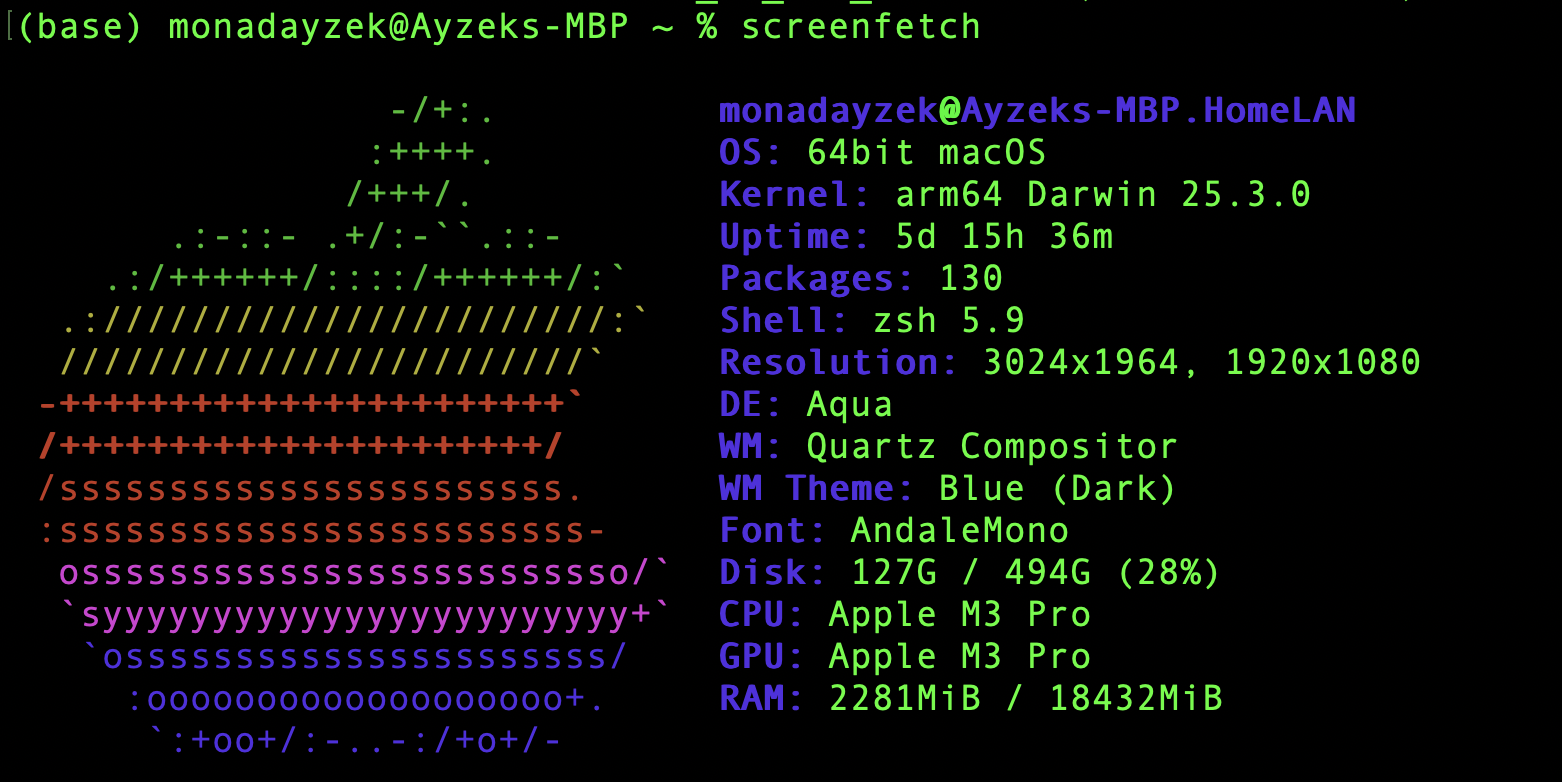
\includegraphics[width=0.60\linewidth]{img/lab-1/macos.png}
    \caption{Информация об операционной системе (ноутбук)}
    \label{fig:macos}
\end{figure}

\begin{figure}[H]
    \centering
    
\includegraphics[width=0.28\linewidth]{img/lab-1/ios.png}
    \caption{Информация об операционной системе (смартфон)}
    \label{fig:ios}
\end{figure}

\subsubsection{Поиск уязвимостей ОС ноутбука}
Для поиска уязвимостей операционной системы ноутбука в Банке угроз\cite{bdu}, необходимо указать в поисковике слудющую информацию:
\begin{itemize}
    \item Производитель ПО: Apple;
    \item Тип ПО: Операционная система;
    \item Программное обеспечение: macOS;
    \item Аппаратная платформа: ARM64;
    \item Операционная система: MacOS Tahoe до 26.2 (крайняя версия ФСТЭК);
    \item Уровень опасности$^*$: Критический.
\end{itemize}

* - По поставленновки задачи лабораторной работы №1, требуется выявить \textcolor{red}{критические} уязвимости ПО. 
Если \textcolor{red}{критические} уязвимости не найдены, ищуться уязвимости \textcolor{orange}{высокой} опасности, если нет \textcolor{orange}{высокой} опасности, \textcolor{yellow}{средние} иначе \textcolor{green}{низкие}.

Как видно из рисунка \ref{fig:fstecmacos}, выявлено лишь три уязвимостей, две из которых \textcolor{yellow}{среднего} уровня, и одна \textcolor{green}{низкого} уровня.

\begin{figure}[H]
    \centering
    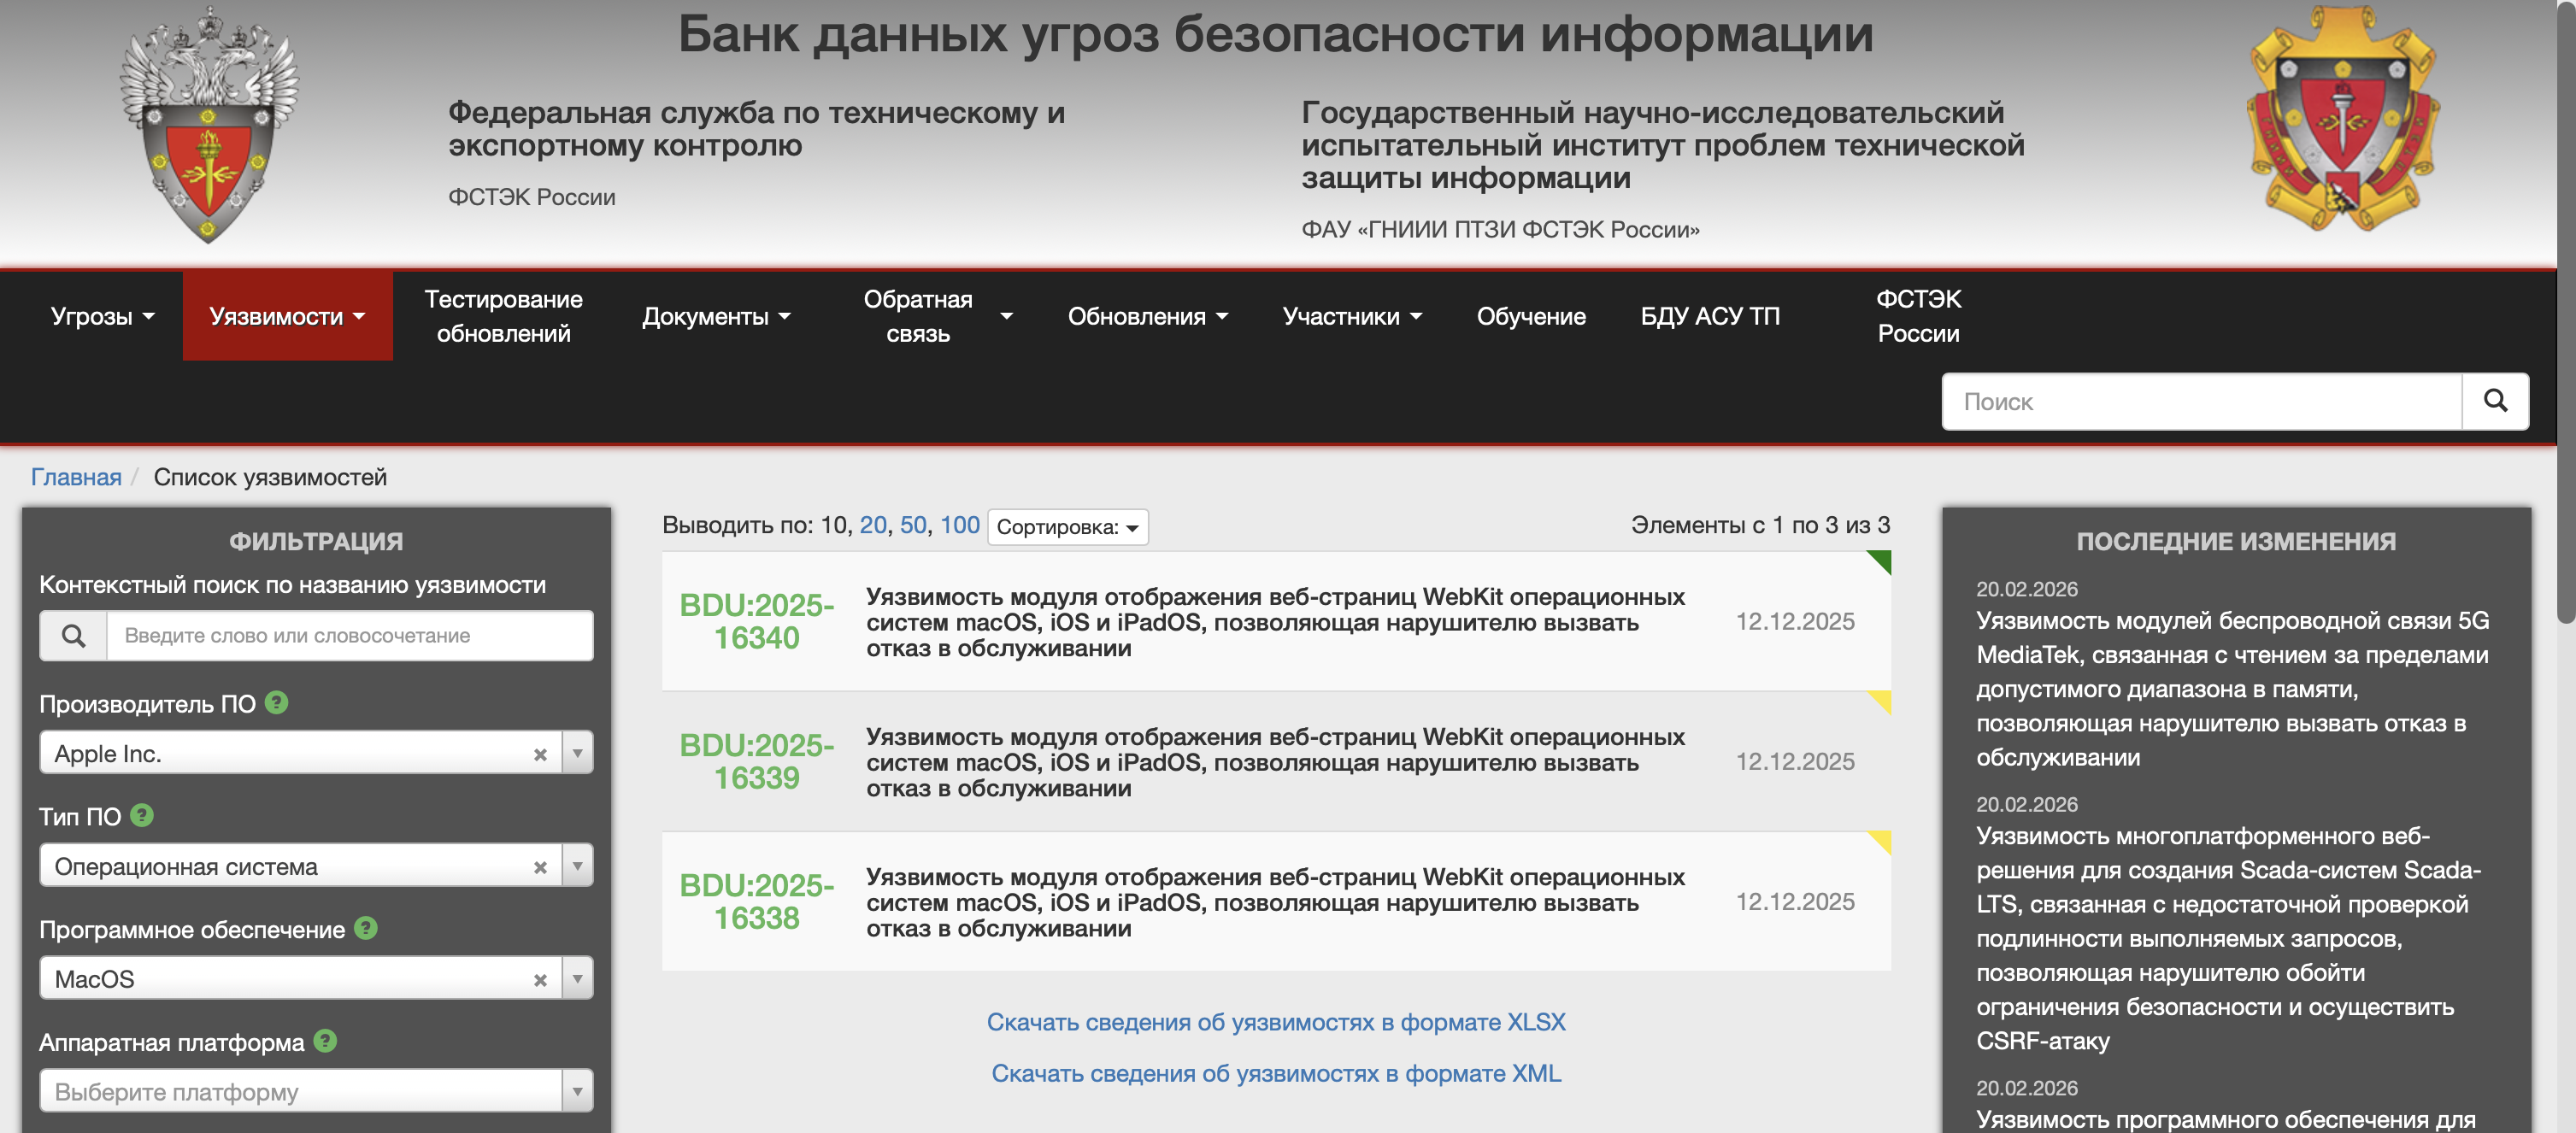
\includegraphics[width=0.60\linewidth]{img/lab-1/fstecmacos.png}
    \caption{Уязвимости macOS 26.2}
    \label{fig:fstecmacos}
\end{figure}

Все уязвимости связанны с отображением страниц WebKit причем модули уязвимы как для macOS так и для iOS и iPadOS. 
Уязвимость позваляет злоумышленнику вызвать отказ в обслуживании. 

Более подробное описание двух средних уязвимостей представлено на рисунке \ref{fig:fstecmacos1full}, и \ref{fig:fstecmacos2full}, для низкого уровня на рисунке \ref{fig:fstecmacosfullgreen}.

\begin{figure}[H]
    \centering
    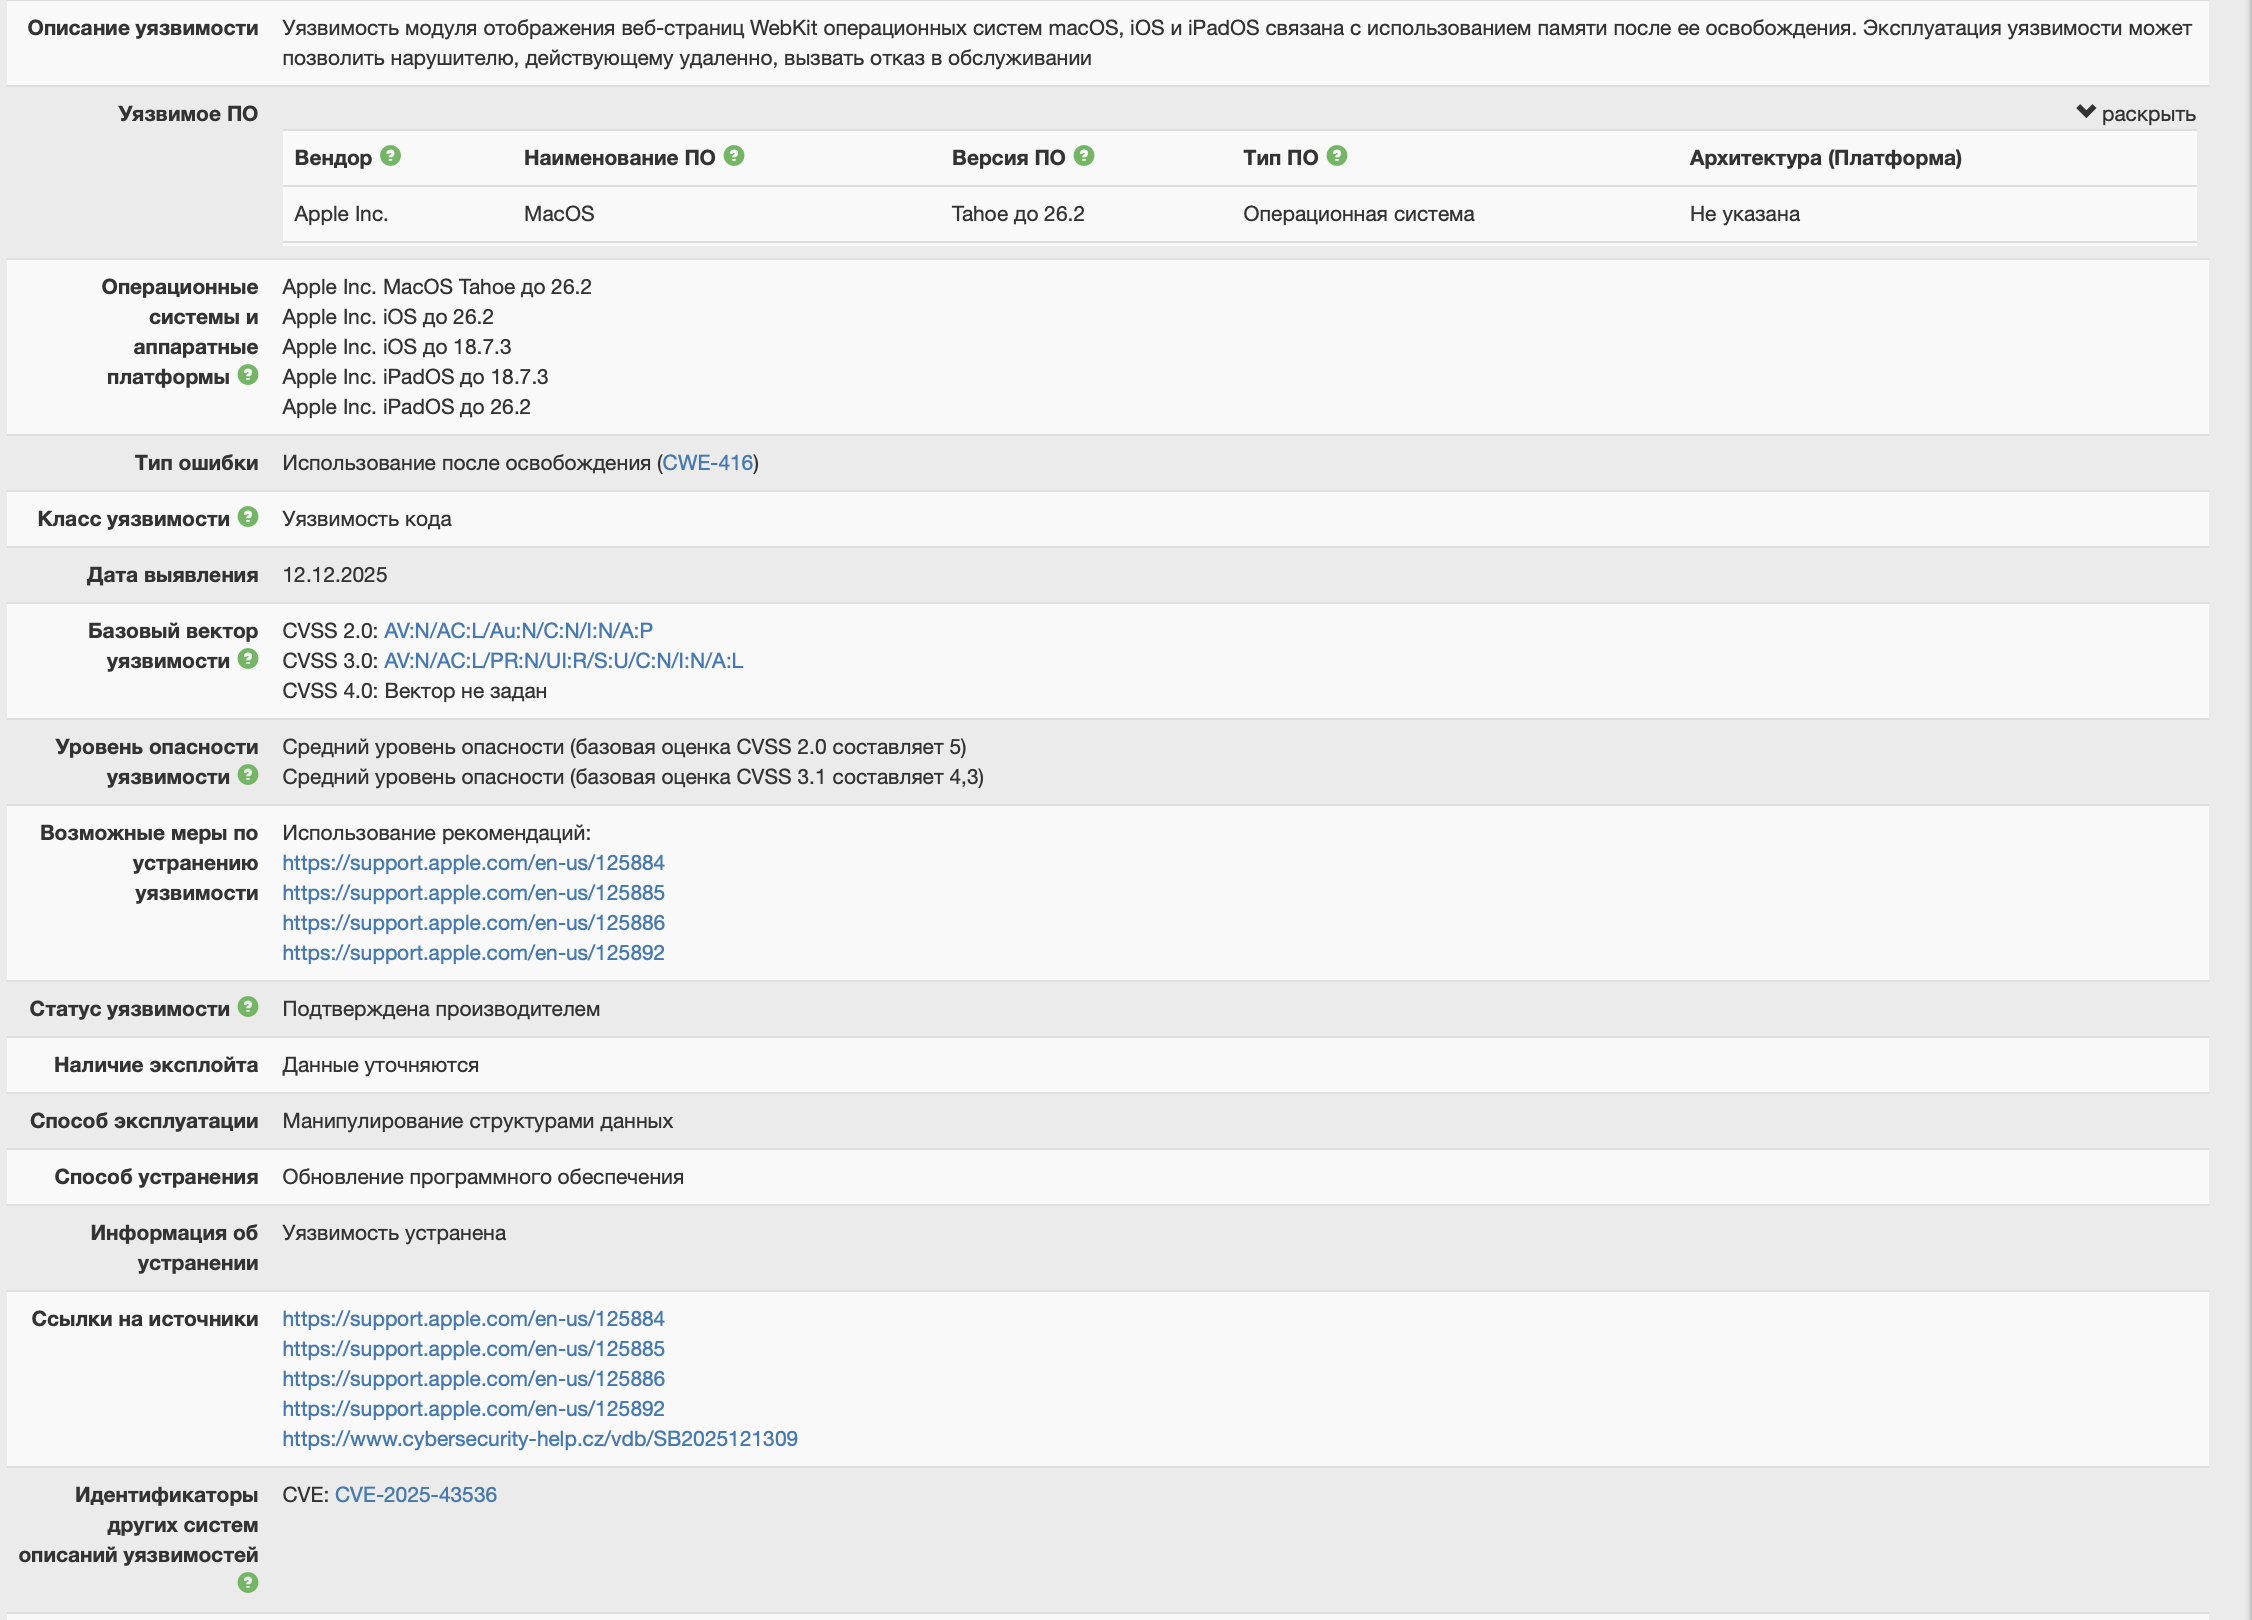
\includegraphics[width=0.60\linewidth]{img/lab-1/fstecmacos2full.png}
    \caption{Уязвимость среднего уровня BDU:2025-16339}
    \label{fig:fstecmacos2full}
\end{figure}

\begin{figure}[H]
    \centering
    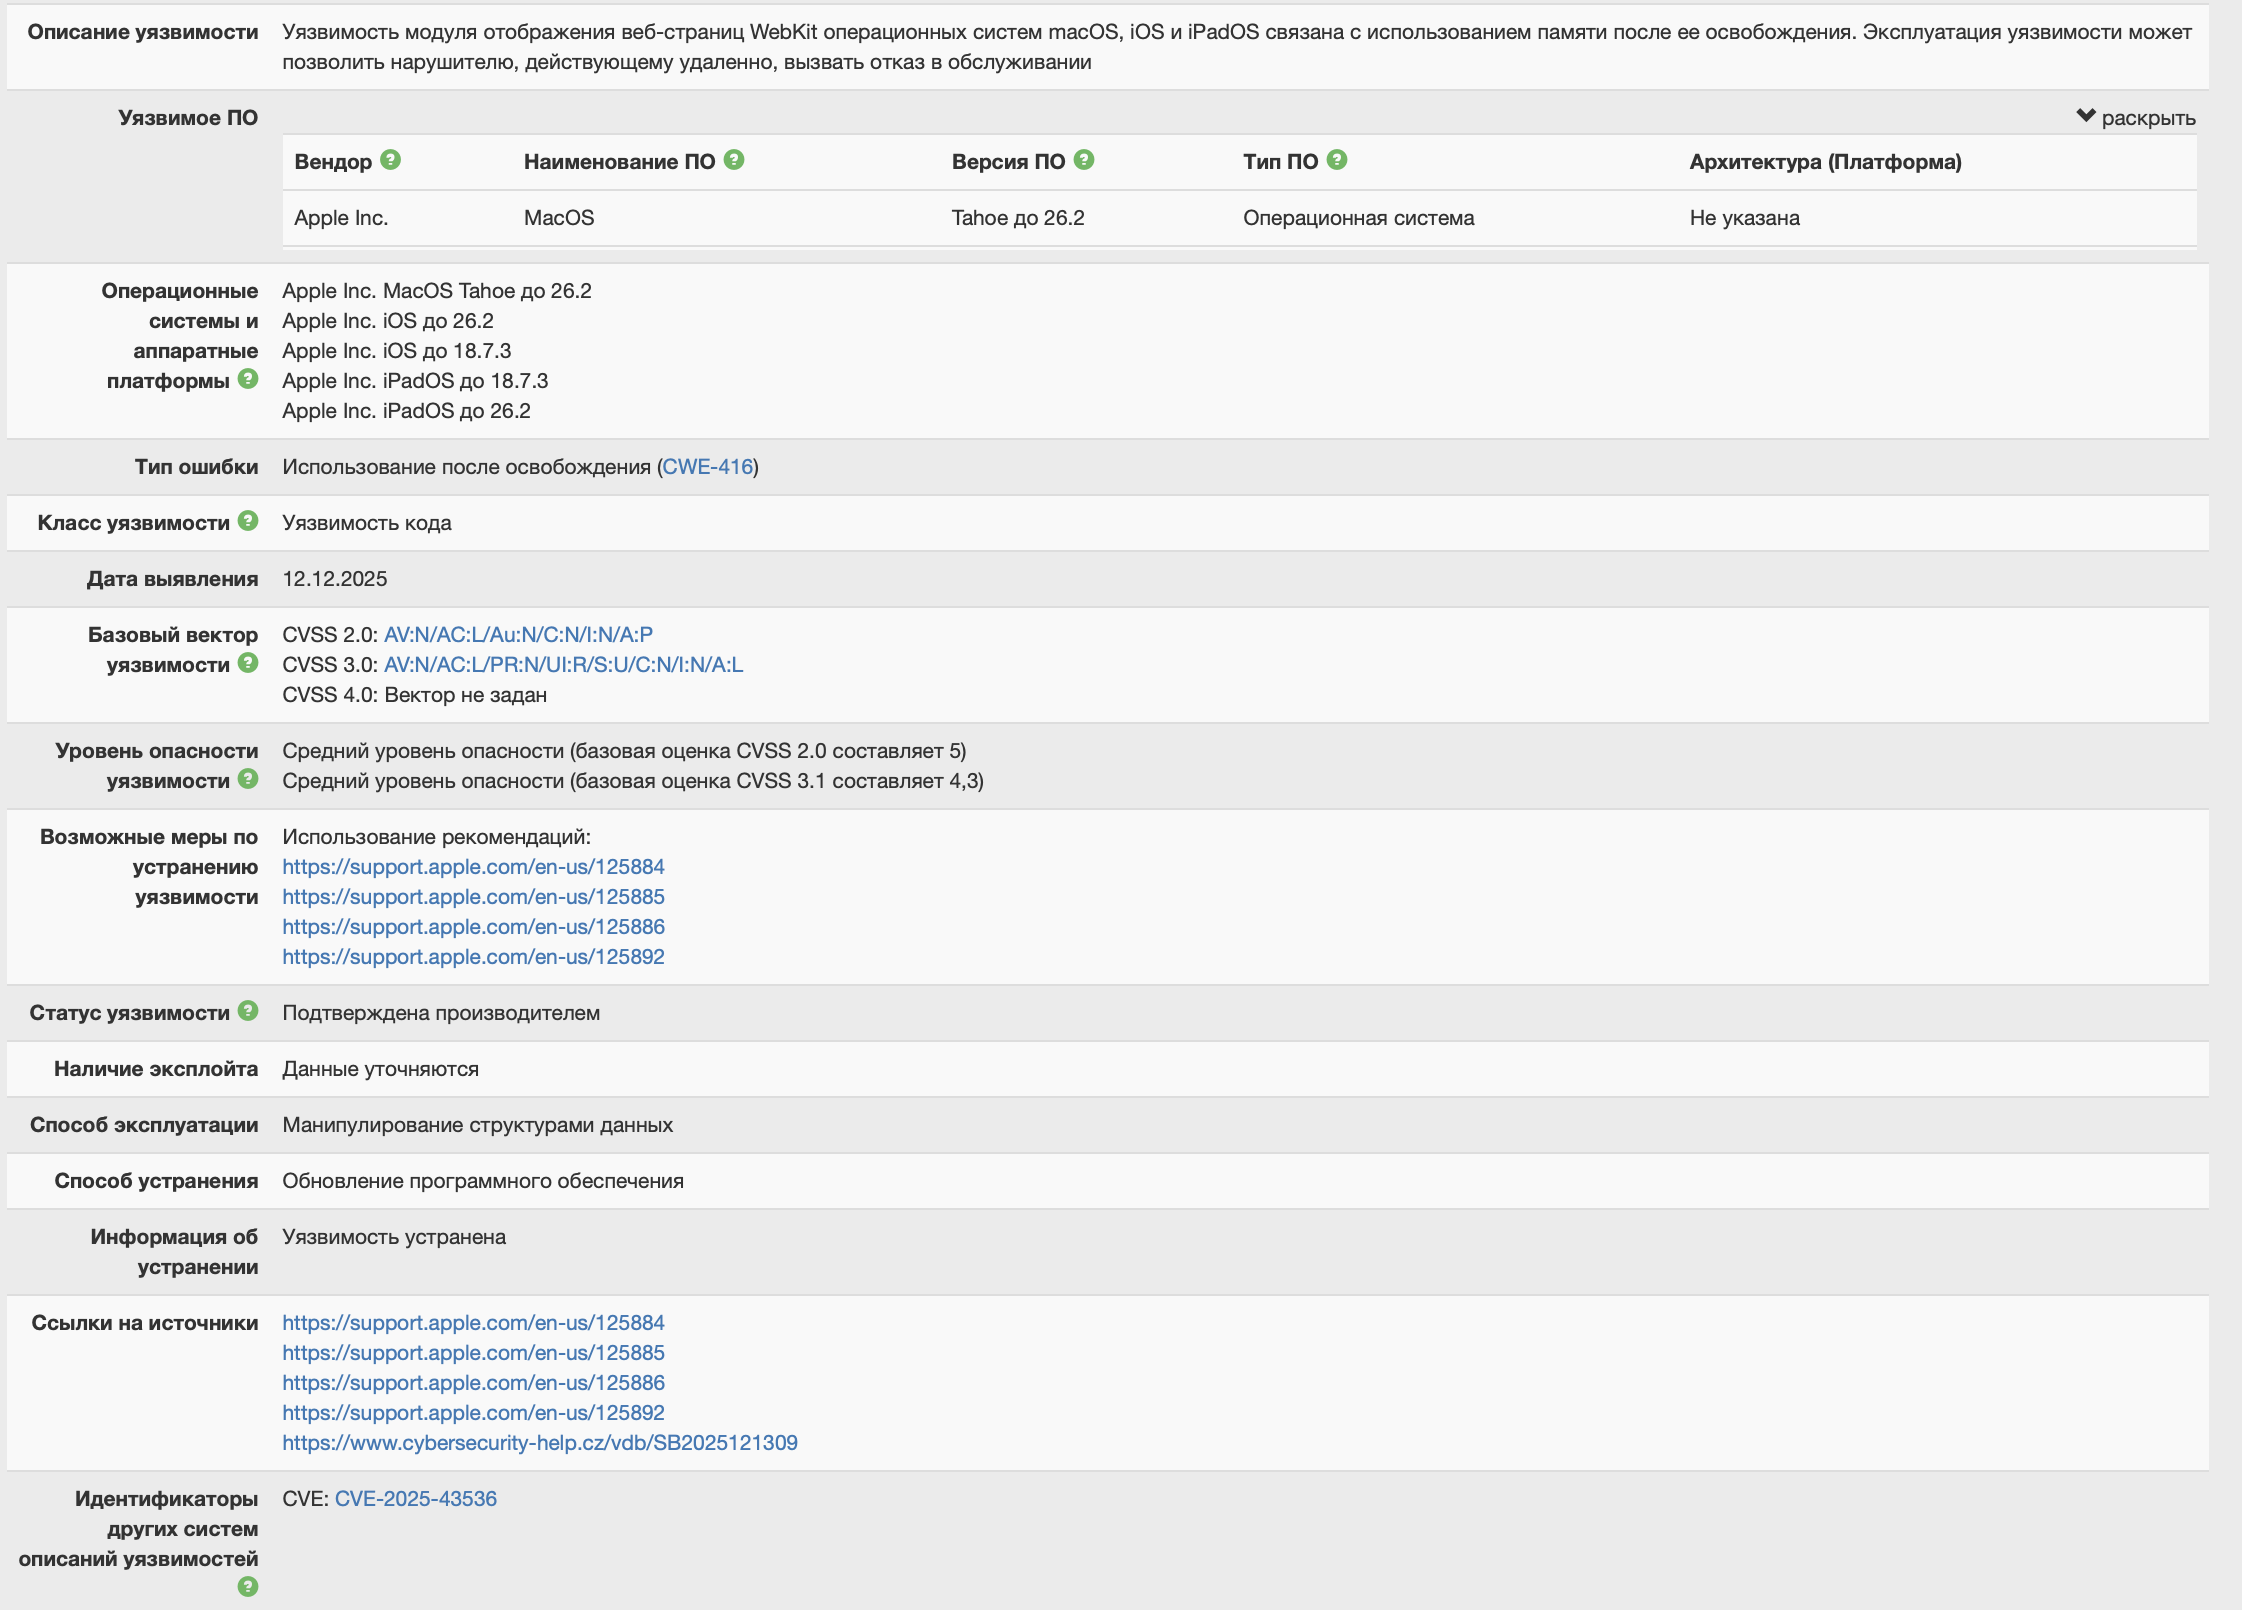
\includegraphics[width=0.60\linewidth]{img/lab-1/fstecmacos1full.png}
    \caption{Уязвимость среднего уровня BDU:2025-16338}
    \label{fig:fstecmacos1full}
\end{figure}

\begin{figure}[H]
    \centering
    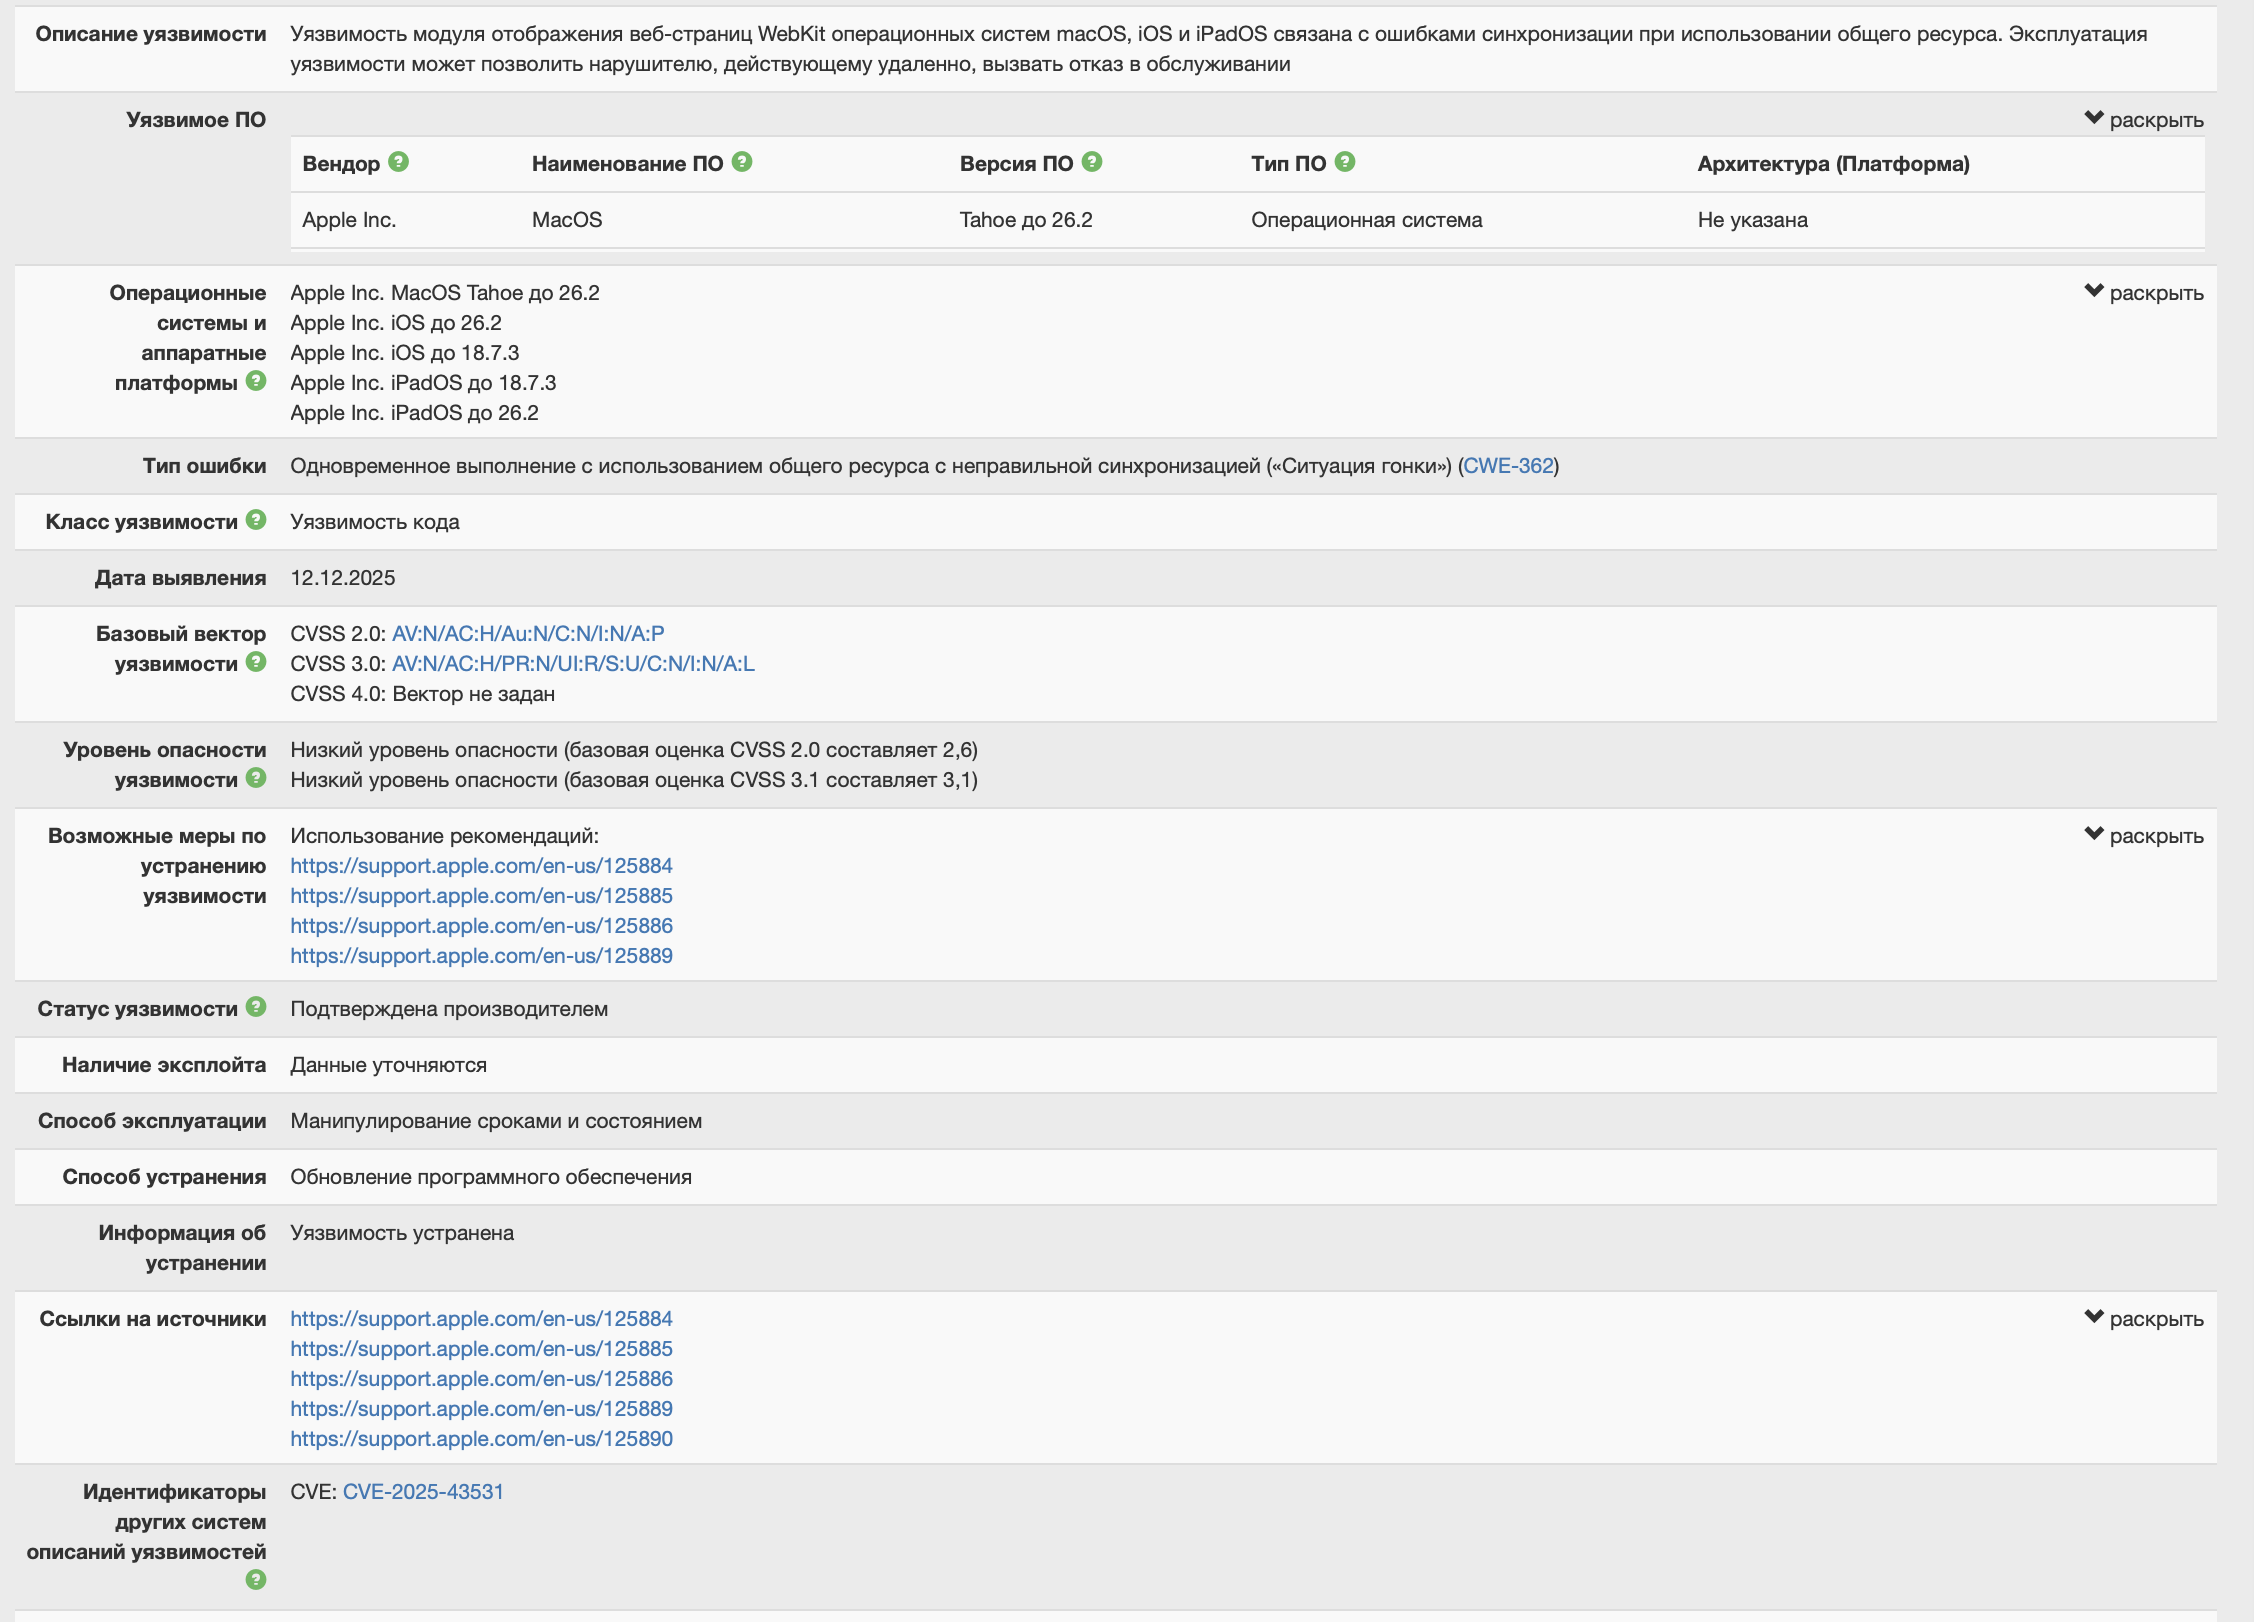
\includegraphics[width=0.60\linewidth]{img/lab-1/fstecmacosfullgreen.png}
    \caption{Уязвимость низкого уровня BDU:2025-16340}
    \label{fig:fstecmacosfullgreen}
\end{figure}

Как видно, все три уязвимости относятся к типу уязвимости кода, и неотличимы друг от друга.

Ниже представленны таблица \ref{tab:cvss2}, и таблица \ref{tab:cvss3}, где перечислены все метрики векторов уязвимостей для CVSS 2.0 и CVSS 3.0 (см. Таб. \ref{tab:terms}) соответственно, с пояснением:

\begin{table}[H]
\centering
\small 
\caption{Метрики вектора уязвимости CVSS 2.0}
\label{tab:cvss2}
\begin{tabularx}{\textwidth}{|l|l|X|}
\hline
\textbf{Аббревиатура} & \textbf{Расшифровка} & \textbf{Значения и смысл} \\
\hline
AV  & Access Vector (вектор доступа) & \textbf{Local (L)} - локальный доступ; \textbf{Adjacent Network (A)} - доступ из смежной сети; \textbf{Network (N)} - сетевой доступ. Определяет способ взаимодействия с системой. \\
\hline
AC  & Access Complexity (сложность доступа) & \textbf{High (H)} - высокая; \textbf{Medium (M)} - средняя; \textbf{Low (L)} - низкая. Характеризует условия, необходимые для эксплуатации. \\
\hline
Au  & Authentication (аутентификация) & \textbf{Multiple (M)} - множественная; \textbf{Single (S)} - единственная; \textbf{None (N)} - не требуется. Указывает на необходимость подтверждения подлинности. \\
\hline
C   & Confidentiality Impact (влияние на конфиденциальность) & \textbf{None (N)} - отсутствует; \textbf{Partial (P)} - частичное; \textbf{Complete (C)} - полное. Степень раскрытия информации. \\
\hline
I   & Integrity Impact (влияние на целостность) & \textbf{None (N)} - отсутствует; \textbf{Partial (P)} - частичное; \textbf{Complete (C)} - полное. Возможность искажения данных. \\
\hline
A   & Availability Impact (влияние на доступность) & \textbf{None (N)} - отсутствует; \textbf{Partial (P)} - частичное; \textbf{Complete (C)} - полное. Степень нарушения доступности сервиса. \\
\hline
\end{tabularx}
\end{table}

\begin{table}[H]
\centering
\small
\caption{Метрики вектора уязвимости CVSS 3.0}
\label{tab:cvss3}
\begin{tabularx}{\textwidth}{|l|l|X|}
\hline
\textbf{Аббревиатура} & \textbf{Расшифровка} & \textbf{Значения и смысл} \\
\hline
AV  & Attack Vector (вектор атаки) & \textbf{Network (N)} - сетевой; \textbf{Adjacent (A)} - из смежной сети; \textbf{Local (L)} - локальный; \textbf{Physical (P)} - физический. Отражает удалённость атаки. \\
\hline
AC  & Attack Complexity (сложность атаки) & \textbf{Low (L)} - низкая; \textbf{High (H)} - высокая. Наличие условий вне контроля атакующего. \\
\hline
PR  & Privileges Required (необходимые привилегии) & \textbf{None (N)} - не требуются; \textbf{Low (L)} - низкие; \textbf{High (H)} - высокие. Уровень прав доступа до атаки. \\
\hline
UI  & User Interaction (взаимодействие с пользователем) & \textbf{None (N)} - не требуется; \textbf{Required (R)} - требуется. Участие другого лица в успешной атаке. \\
\hline
S   & Scope (область действия) & \textbf{Unchanged (U)} - не изменяется; \textbf{Changed (C)} - изменяется. Возможность воздействия на другие компоненты. \\
\hline
C   & Confidentiality Impact (влияние на конфиденциальность) & \textbf{High (H)} - высокое; \textbf{Low (L)} - низкое; \textbf{None (N)} - отсутствует. Степень потери конфиденциальности. \\
\hline
I   & Integrity Impact (влияние на целостность) & \textbf{High (H)} - высокое; \textbf{Low (L)} - низкое; \textbf{None (N)} - отсутствует. Возможность модификации данных. \\
\hline
A   & Availability Impact (влияние на доступность) & \textbf{High (H)} - высокое; \textbf{Low (L)} - низкое; \textbf{None (N)} - отсутствует. Степень нарушения доступности. \\
\hline
\end{tabularx}
\end{table}


Для более детального анализа, стоит расмотреть базойвый вектор уязвимости каждой уязвимости:

\begin{itemize}
    \item BDU:2025-16338: \begin{itemize}
        \item CVSS 2.0: AV:N/AC:L/Au:N/C:N/I:N/A:P (Оценка 5)
        \item CVSS 3.0: AV:N/AC:L/PR:N/UI:R/S:U/C:N/I:N/A:L (Оценка 4,3)
        \item CVSS 4.0: -
    \end{itemize} 
    \item BDU:2025-16339: \begin{itemize}
        \item CVSS 2.0: AV:N/AC:L/Au:N/C:N/I:N/A:P (Оценка 5)
        \item CVSS 3.0: AV:N/AC:L/PR:N/UI:R/S:U/C:N/I:N/A:L (Оценка 4,3)
        \item CVSS 4.0: -
    \end{itemize} 
    \item BDU:2025-16340: \begin{itemize}
        \item CVSS 2.0: AV:N/AC:H/Au:N/C:N/I:N/A:P (Оценка 2,6)
        \item CVSS 3.0: AV:N/AC:H/PR:N/UI:R/S:U/C:N/I:N/A:L (Оценка 3,1)
        \item CVSS 4.0: -
    \end{itemize} 
\end{itemize}

Так как вектора идентичны для средних уровней можно расписать их едино:

\textbf{CVSS 2.0: AV - способ получения доступа: N - сетевой/ AC - сложность получения доступа: L - низкая/ Au - аутентификация : N - не требуется/
C - влияние на конфиденциальность: N - не оказывает/ I - влияние на целостность: N - не оказывает/ A - влияние на доступность: P - частичное.}

\emph{Таким образом для CVSS 2.0, можно прочесть уязвимость как - сетевое подключение доступа с низкой сложнастью без аутентификации не влияющая на конфиденциальность не оказывающая влияние на целостность и частично влияющая на доступность.}

\textbf{CVSS 3.0: AV - Вектор атаки: N - сетевой/ AC - сложность атаки: L - низкая/ PR - уровень привелегий: N - не требуется/ UI - взаимодействие с пользователем: R - требуется/ S - влияние на другие компоненты системы: U - не оказывает/ C - влияние на конфиденциальность: N - не оказывает/ I - влияние на целостность: N - не оказыает/ A - влияние на доступность: L - низкое.}

\emph{Таким образом для CVSS 3.0, можно прочесть уязвимость как - сетевой вектор атаки с низкой сложностью, не требующий уровень привелегий с взаимодействием с пользователем, не влияющая на другие компоненты, не влияющая на конфиденциальность, без оказания влияния на целостность с низким влиянием на доступность.}

Вектор для низкого уровня уязвимости отличается лишь пунтом \guillemetleft  сложность атаки\guillemetright (AC), и имеет индекст H, то есть высокая сложность. Таким образом для низкого уровня уязвимости:

\textbf{CVSS 2.0: AV - способ получения доступа: N - сетевой/ AC - сложность получения доступа: H - высокая/ Au - аутентификация : N - не требуется/
C - влияние на конфиденциальность: N - не оказывает/ I - влияние на целостность: N - не оказывает/ A - влияние на доступность: P - частичное.}

\emph{То есть - сетевое подключение доступа с высокой сложнастью без аутентификации не влияющая на конфиденциальность не оказывающая влияние на целостность и частично влияющая на доступность.}

\textbf{CVSS 3.0: AV - Вектор атаки: N - сетевой/ AC - сложность атаки: H - высокая/ PR - уровень привелегий: N - не требуется/ UI - взаимодействие с пользователем: R - требуется/ S - влияние на другие компоненты системы: U - не оказывает/ C - влияние на конфиденциальность: N - не оказывает/ I - влияние на целостность: N - не оказыает/ A - влияние на доступность: L - низкое.}

\emph{То есть - сетевой вектор атаки с высокой сложностью, не требующий уровень привелегий с взаимодействием с пользователем, не влияющая на другие компоненты, не влияющая на конфиденциальность, без оказания влияния на целостность с низким влиянием на доступность.}

\subsubsection{Поиск уязвимостей ОС смартфона}
Для поиска уязвимостей операционной системы смартфона в Банке угроз\cite{bdu}, необходимо указать в поисковике слудющую информацию:

\begin{itemize}
    \item Производитель ПО: Apple;
    \item Тип ПО: Операционная система;
    \item Программное обеспечение: iOS;
    \item Версия ПО: iOS до 26.2 (крайняя версия ФСТЭК);
    \item Уровень опасности: Критический.
\end{itemize}

На рисунке \ref{fig:iosfstec}, видно что для операционной системы iOS, существуют уязвимости критического уровня, которых довольно много (108 критических уязвимостей).

\begin{figure}[H]
    \centering
    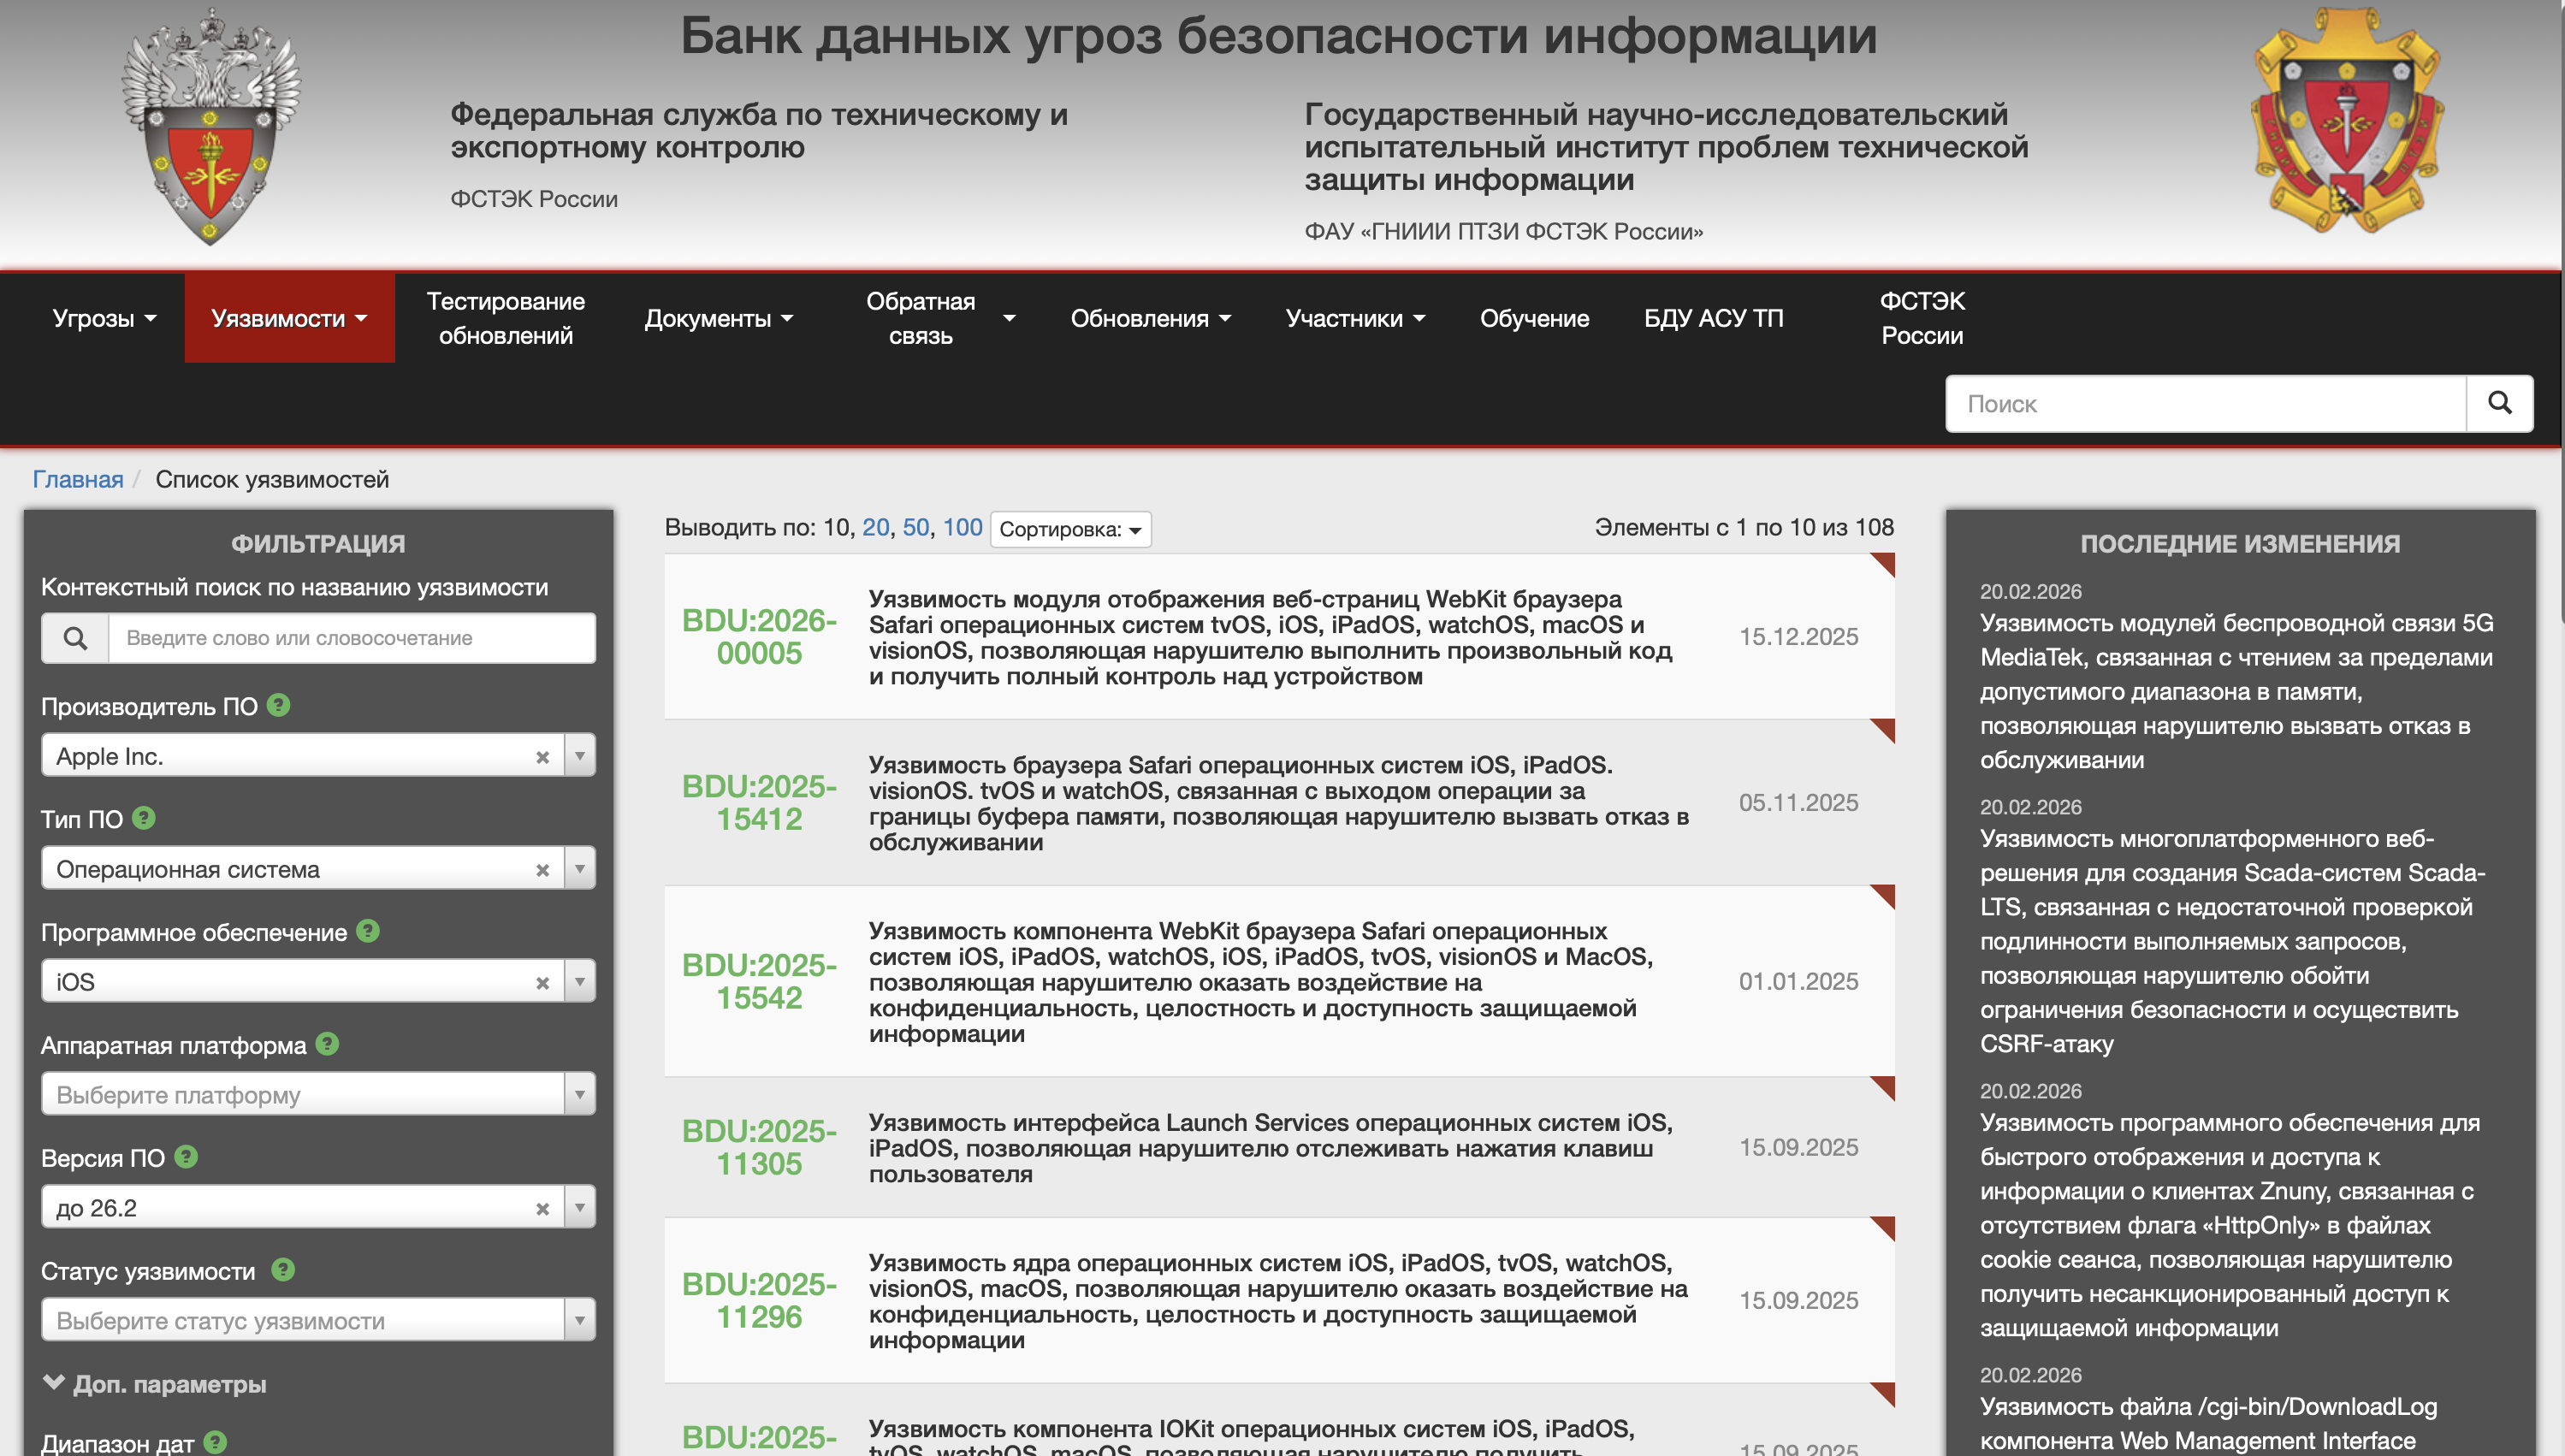
\includegraphics[width=0.60\linewidth]{img/lab-1/iosfstec.png}
    \caption{Критические уязвимости в iOS}
    \label{fig:iosfstec}
\end{figure}

Возьмем первые две из отсортированных по критичности:

\begin{itemize}
    \item BDU:2026-00005;
    \item BDU:2025-15412.
\end{itemize}

BDU:2026-00005, позволяет злоумышленнику, выполнить произвольный код и получить полный контроль над устройством,
а BDU:2025-15412, связанна с выходом операции за границы буфера памяти, которая может позволить злоумышленнику вызвать отказ в обслуживании.

Более подробное описание двух уязвимостей представлены на рисунке \ref{fig:fsteciosfull1}, и \ref{fig:fsteciosfull2}.

\begin{figure}[H]
    \centering
    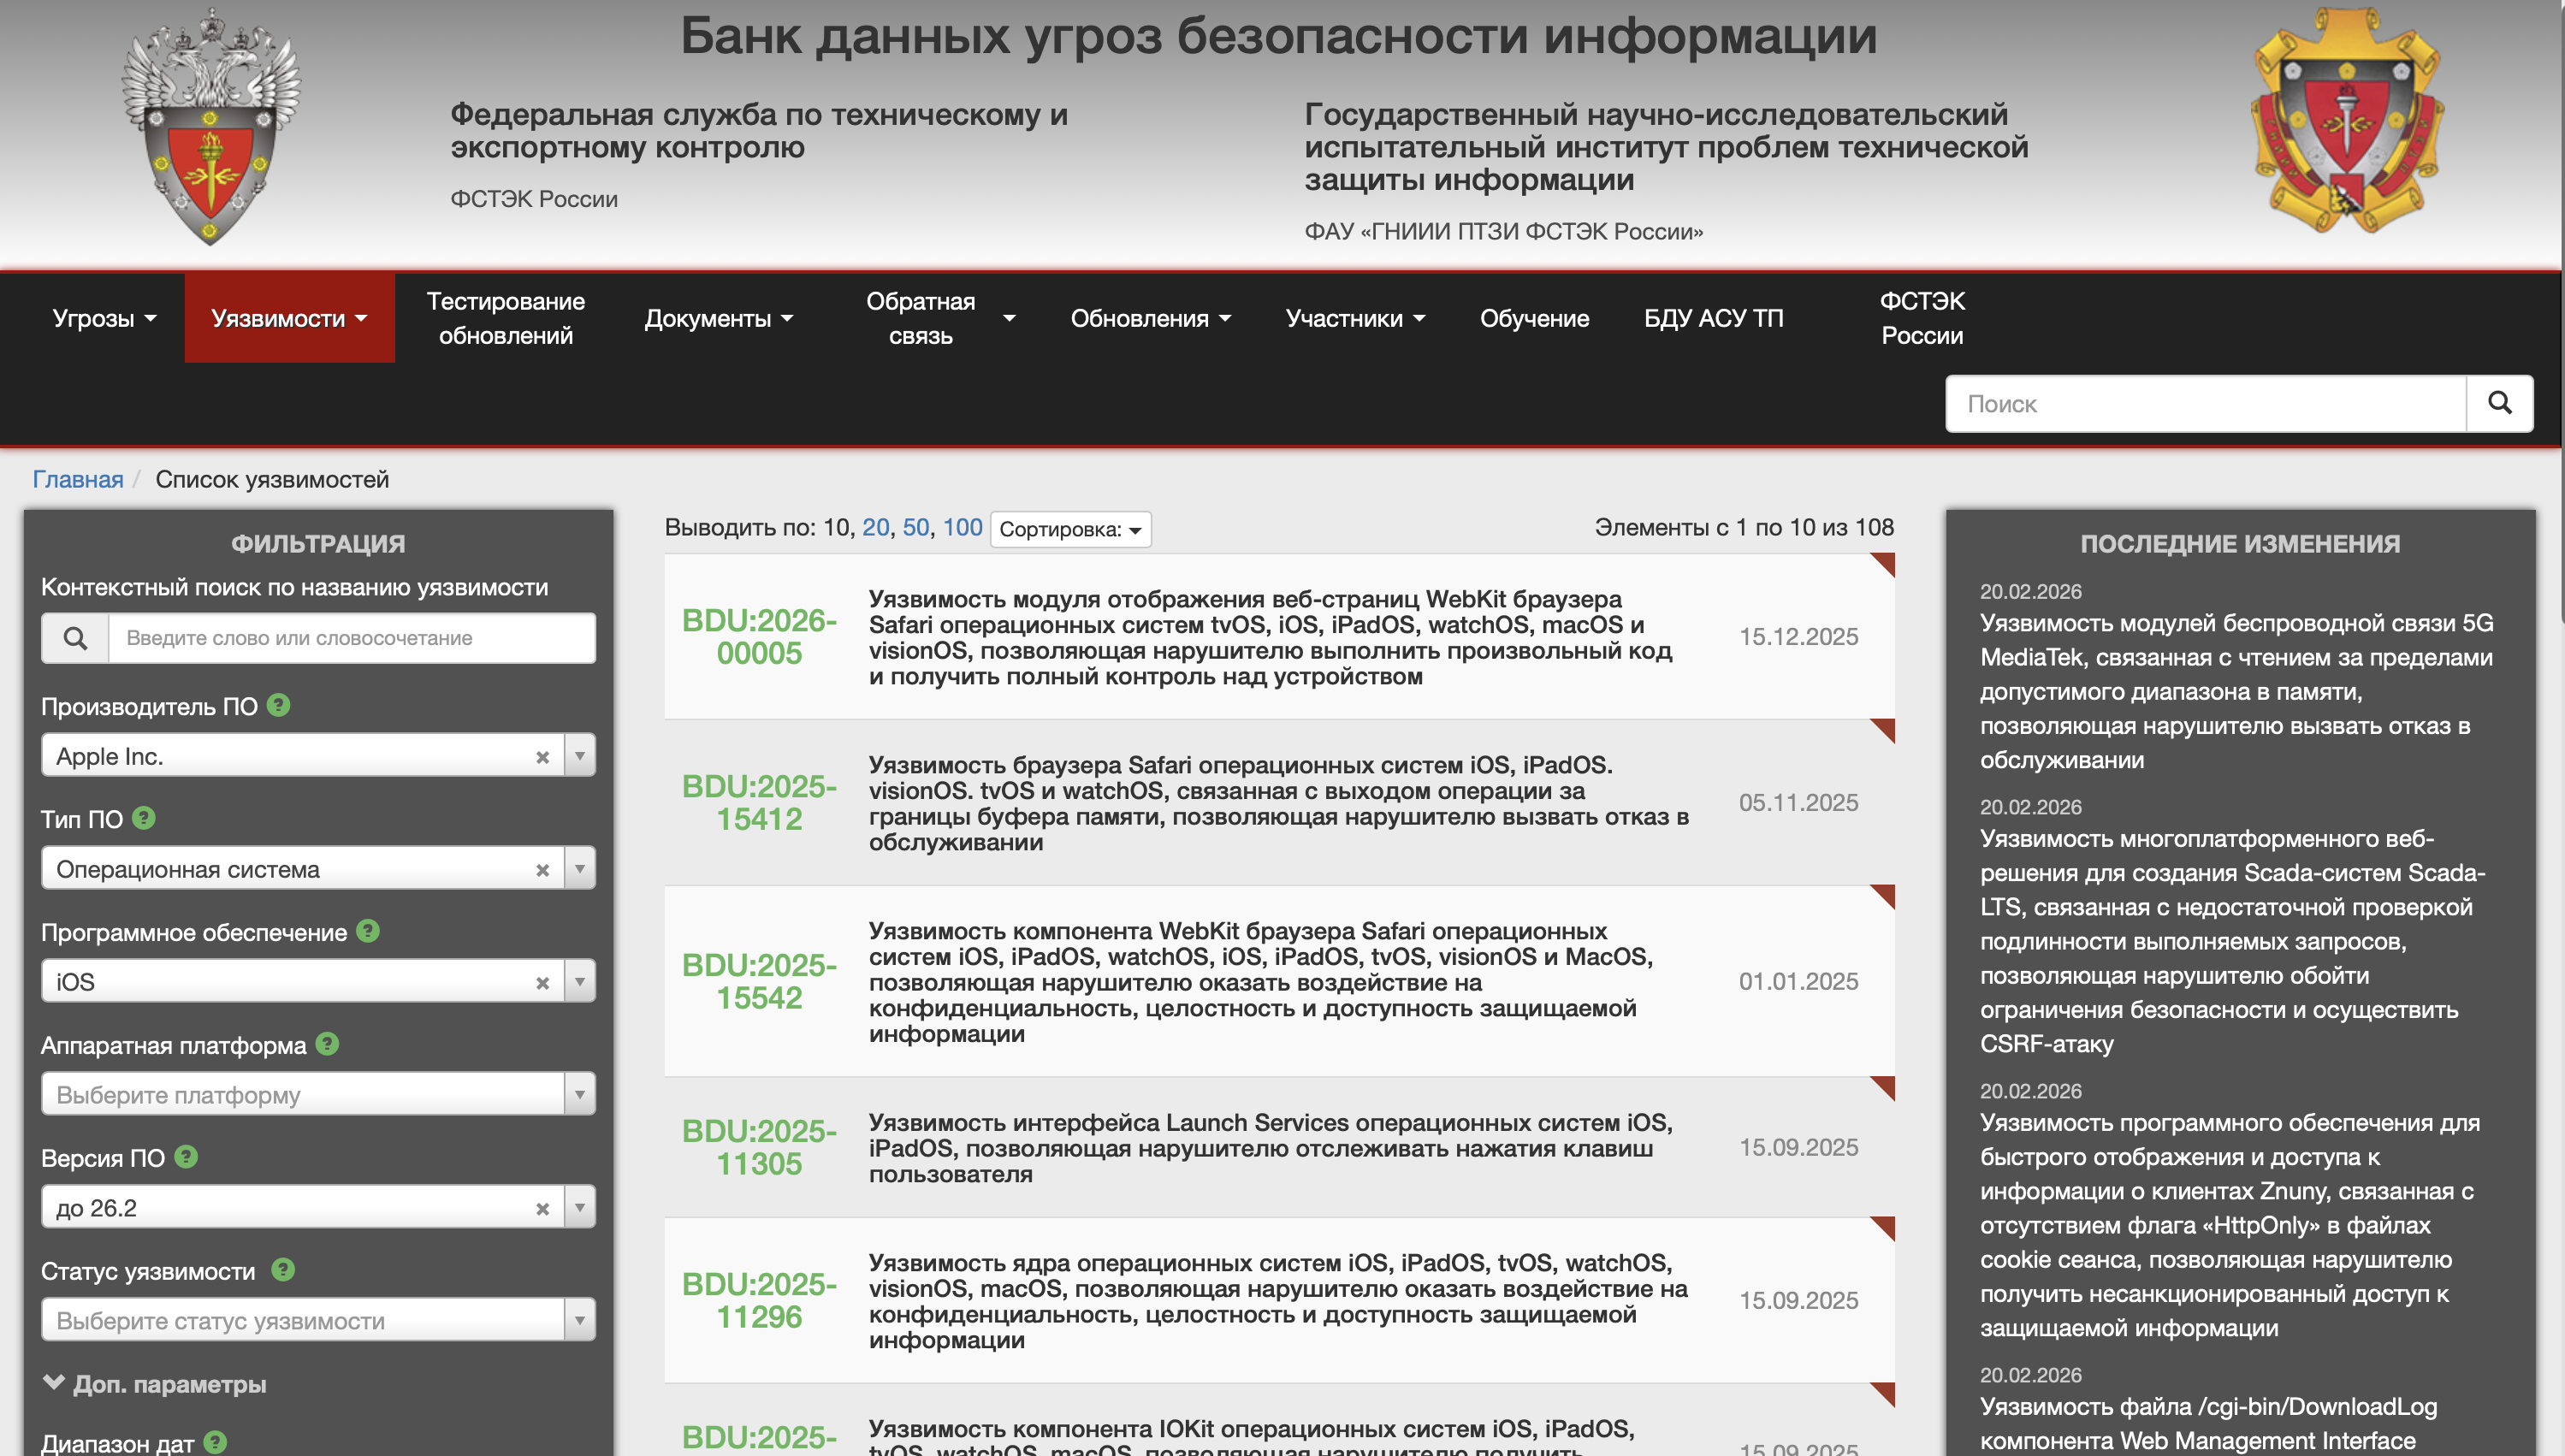
\includegraphics[width=0.60\linewidth]{img/lab-1/iosfstec.png}
    \caption{Уязвимость критического уровня BDU:2026-00005}
    \label{fig:fsteciosfull1}
\end{figure}

\begin{figure}[H]
    \centering
    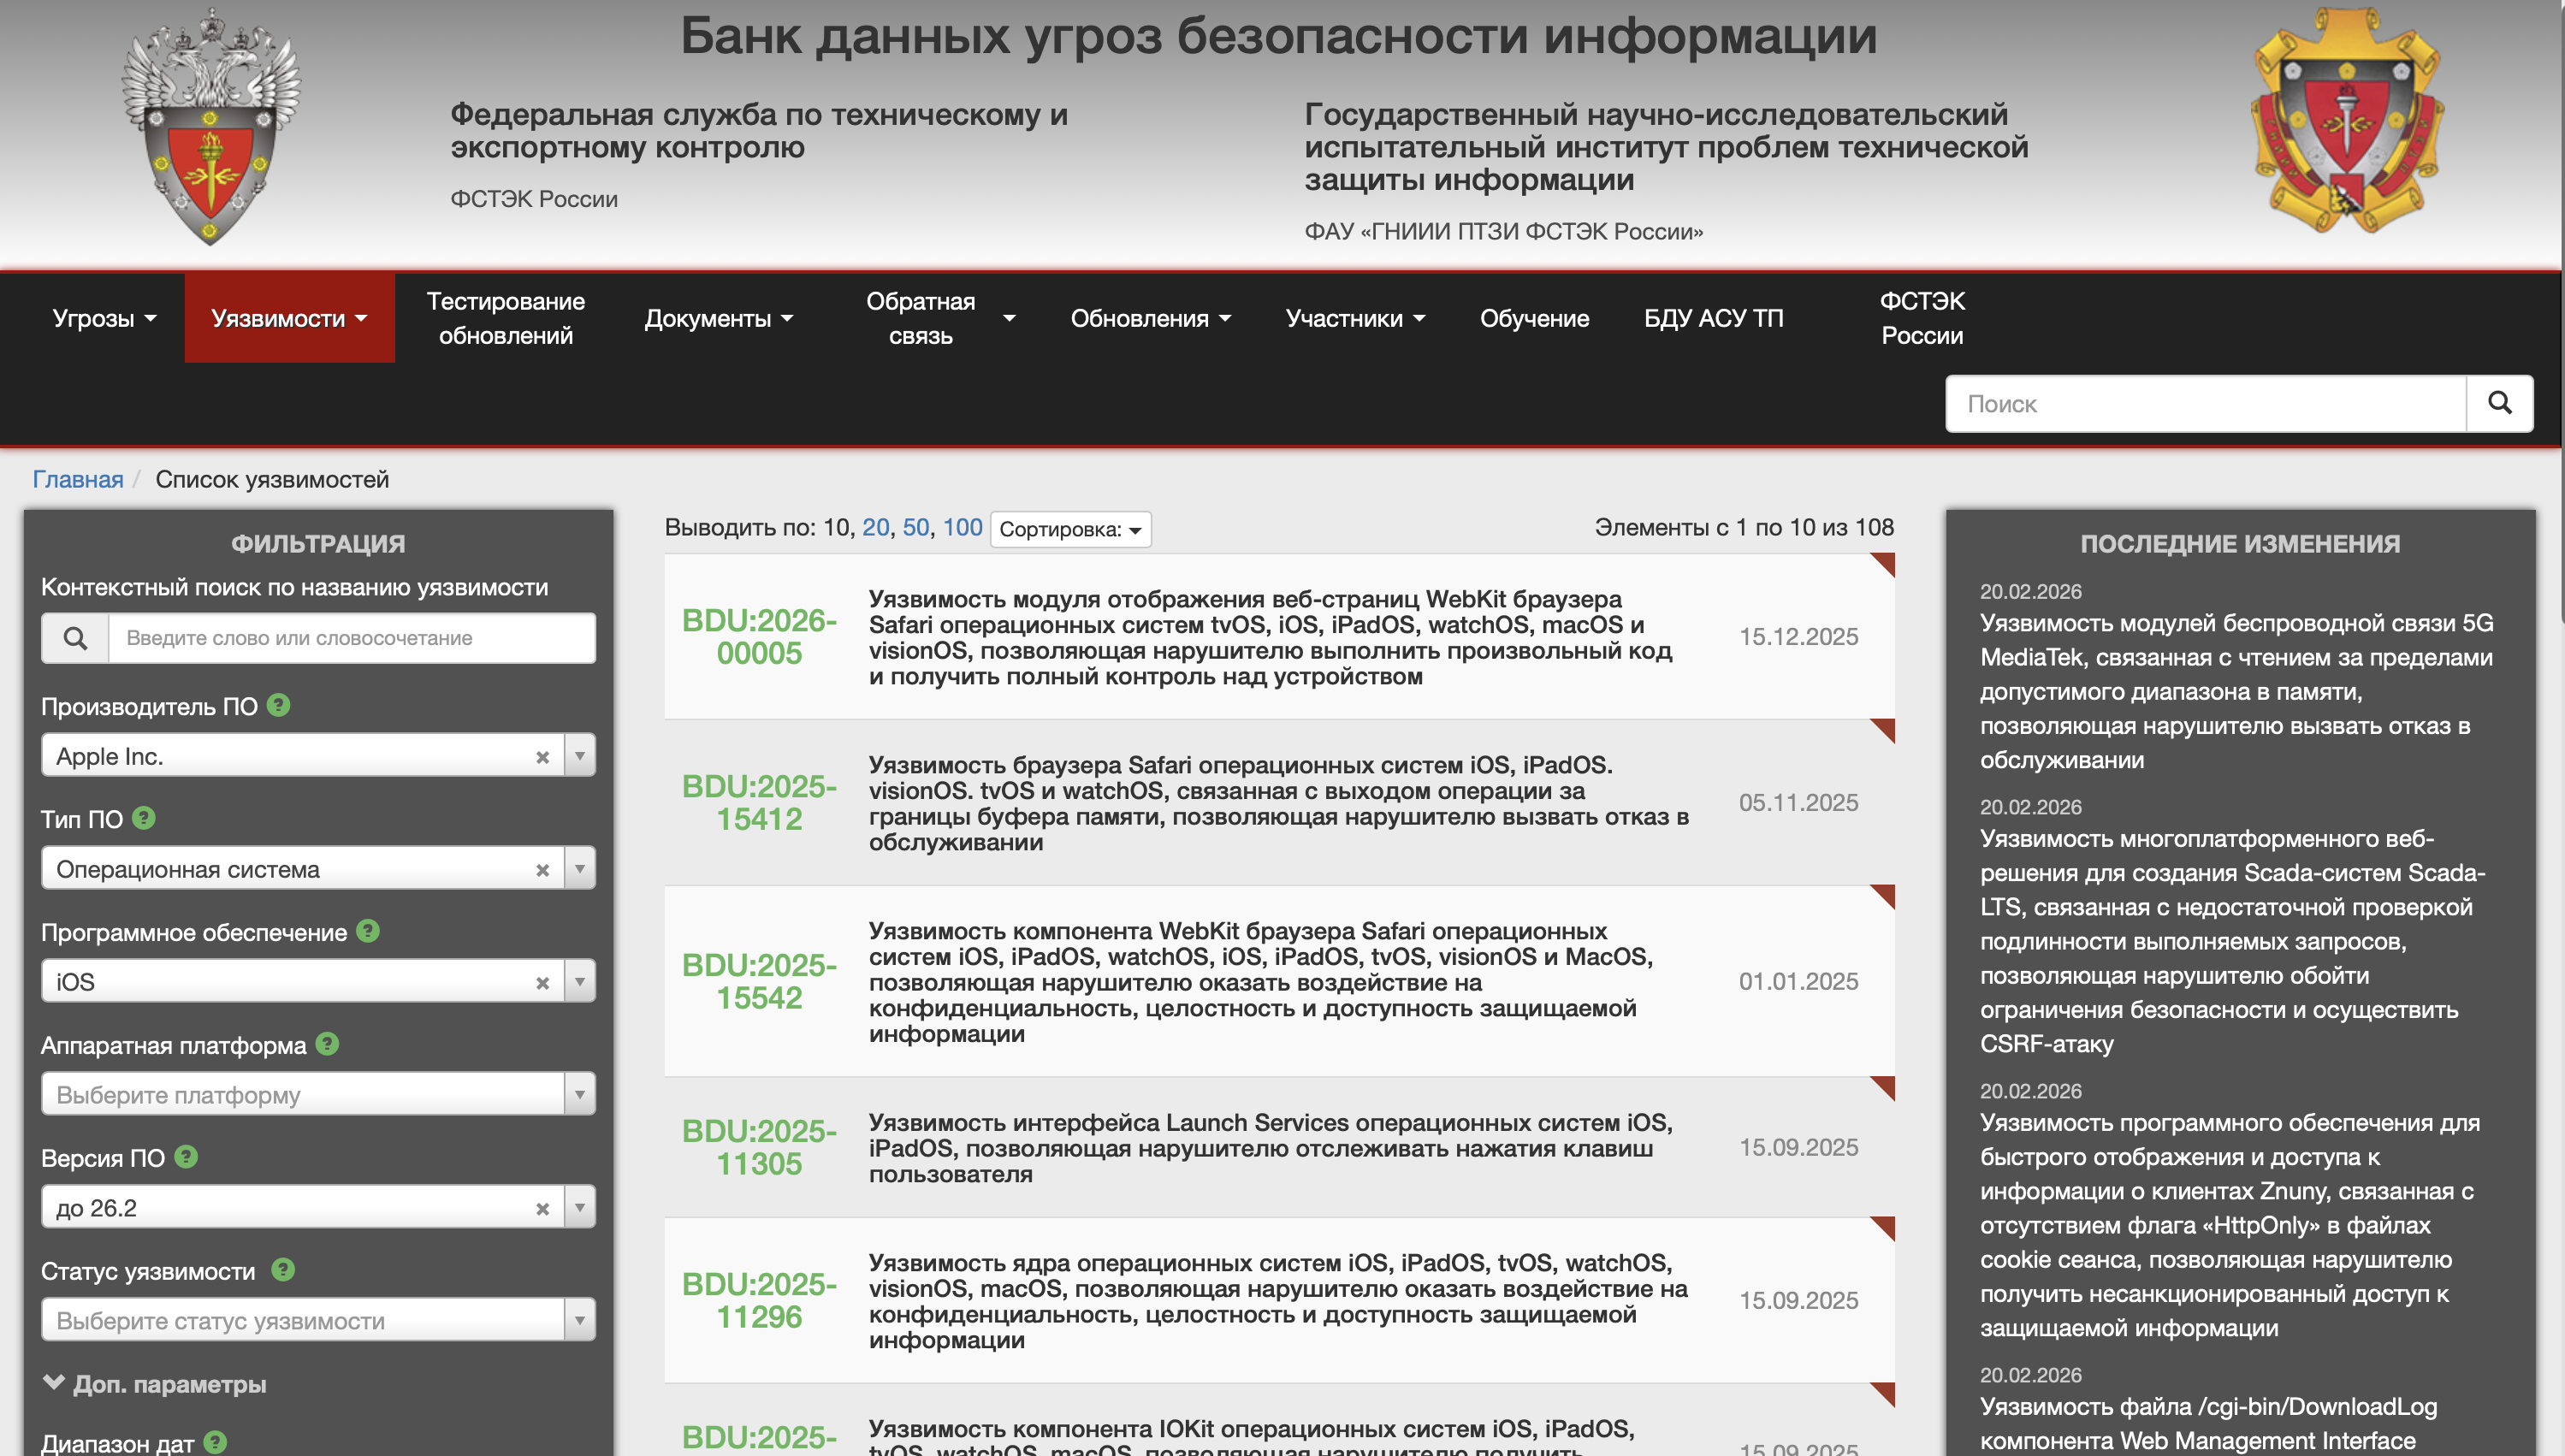
\includegraphics[width=0.60\linewidth]{img/lab-1/iosfstec.png}
    \caption{Уязвимость критического уровня BDU:2025-15412}
    \label{fig:fsteciosfull2}
\end{figure}

Так же опишем их базовые вектора уязвимостей:

\begin{itemize}
    \item BDU:2026-00005: \begin{itemize}
        \item CVSS 2.0: AV:N/AC:L/Au:N/C:C/I:C/A:C
        \item CVSS 3.0: AV:N/AC:L/PR:N/UI:R/S:U/C:H/I:H/A:H
        \item CVSS 4.0: - 
    \end{itemize}
    \item BDU:2025-15412: \begin{itemize}
        \item CVSS 2.0: AV:N/AC:L/Au:N/C:C/I:C/A:C
        \item CVSS 3.0: AV:N/AC:L/PR:N/UI:R/S:U/C:H/I:H/A:H
        \item CVSS 4.0: - 
    \end{itemize}
\end{itemize}

Вектора полностью идентичны, их можно описать едино:

\textbf{CVSS 2.0: AV - способ получения доступа: N - сетевой/ AC - сложность получения доступа: L - низкая/
Au - аутентификация: N - не требуется/ C - влияние на конфиденциальность: C - полное/ I - влияние
на целостность: C - полное/ A - влияние на доступность: C - полное.}

\emph{То есть это сетевой способ получения доступа с низкой сложностью, без аутентификации с влиянием на конфиденциальность, целостность и доступность.}

\textbf{CVSS 3.0: AV - вектор атаки: N - сетевой/ AC - сложность атаки: L - низкая/ PR - уровень привелегий: N - не требуется/ UI - взаимодействие с пользователем: R - требуется/ S - влияние на другие компоненты:
U - не оказывает/ C - влияние на конфиденциальность: H - высокое/ I - влияние
на целостность: H - высокое/ A - влияние на доступность: H - высокое.}

\emph{То есть сетевая атака с низкой сложностью, без требования привелегий, со взаимодействием с пользователем, не влияющий на другие компоненты, высоко влияющий на конфиденциальность, целостность и доступность.}

\subsection{Меры для устранения найденных уязвимостей}
Ниже описаны мервы для устранения найденных уязвимостей для операционных систем macOS и iOS соответственно.
\subsubsection{macOS}
Среди найденных уязвимостей для macOS 26.2, в разделе \guillemetleft  Способ устранения\guillemetright Банка угроз\cite{bdu}, является обновление программного обеспечения,
так как модуль WebKit, для пользователя является не контролируемым модулем (нет прямого доступа).

Такой способ касается всех найденных уязвимостей (BDU:2025-16340, BDU:2025-16338, BDU:2025-16339).

По выходу macOS версии 26.3, будет совершено обновление, во избежания использования злоумышленником данных уязвимостей.

\subsubsection{iOS}
Способом устранения в Банке угроз\cite{bdu}, для уязвимости BDU:2026-00005 - рекомендуется обновление программного обеспечения. 
Так же по выходу iOS версии 26.3, будет совершено обновление программного обеспечения.

Для уязвимости BDU:2025-15412, в подробном описании уязвимости в Банке угроз\cite{bdu}, рекомендуется обновление программного обеспечения, 
так же стоит отметить, что уязвимость (исходя из вектора уязвимостей), требует взаимодействия с пользователем, что требует от пользователя 
бдительности. 

По выходу iOS версии 26.3, будет совершено обновление программного обеспечения, во избежания уязвимостей и возможных угроз.

\subsection*{Заключение}
\addcontentsline{toc}{subsection}{Заключение лабораторной работы №1}
В ходе выполнения лабораторной работы №1, был изучен Банк угроз ФСТЭК\cite{bdu}, в котором были выявлины уязвимости для имеющихся операционных систем ноутбука (macOS) и смартфона (iOS). 
В ходе исследования уязвимостей, было выявлено, что операционная система macOS, достаточно хорошо защищена, так как были найденны всего две уязвимости среднего и одна низкого уровня. 
Уязвимости были связаны с модулем WebKit, который мог предоставить частичный доступ к информации. 

Так же было выявлено, что iOS, недостаточно защищенная операционная система, были выявлены критические уязвимости, связанные с полным нарушением безопасности информации, а именно влияние на конфиденциальность, целостность и доступность.
Одна из уязвимостей (относительно новая), была в том, что злоумышленник мог получить полный доступ к устройству, другая же, уязвимостей была связана с утечкой памяти, что позволяло злоумышленнику вызвать отказ в обслуживании.

Все уязвимости найденные как для macOS так и для iOS, устроняются путем обновления программного обеспечения.

\newpage
\section{Разработка и исследование системы аутентификации и авторизации}
\subsection{Введение}
Одним из ключевых механизмов защиты информации от несанкционированного доступа является аутентификация - процесс установления подлинности субъекта на основе предъявленного идентификатора.
В рамках дисциплины \guillemetleft Защита информации\guillemetright исследование методов аутентификации и авторизации позволяет сформировать фундаментальное понимание принципов разграничения доступа к конфиденциальным данным.

Актуальность работы обусловлена необходимостью анализа стойкости различных методов хэширования паролей в зависимости от их длины и сложности.
Проблема слабых паролей остается одной из наиболее распространенных уязвимостей в корпоративных и частных информационных системах.
Изучение эффективности атак методом грубой силы (brute force) на пароли, хэшированные с использованием алгоритма SHA256 ,
позволяет оценить зависимость времени взлома от стойкости алгоритма. 
В данной работе, описана реализация системы защиты утилиты аутентификации и авторизации, и утилиты атаки на пароли. 

\subsection{Постановка задачи}
\subsubsection{Цель}
\begin{itemize}
    \item Разработать систему доступа пользователей к конфиденциальным данным;
    \item Исследовать стойкость паролей к атаке методом грубой силы.
\end{itemize}
\subsubsection{Задачи}
\begin{itemize}
    \item Разработать систему доступа пользователей к конфиденциальным данным, включающую: \begin{enumerate} 
        \item выделенный каталог для хранения всех файлов системы;
        \item утилиту для работы с данными аутентификации и авторизации: паролями и правами доступа;
        \item утилиту доступа к конфиденциальным данным, обеспечивающую аутентификацию и авторизацию пользователя при работе с конфиденциальными данными.
        \end{enumerate}
    \item Разработать программу взлома паролей методом грубой силы и исследовать стойкость паролей в зависимости от длины паролей и алгоритма хэширования.
\end{itemize}

\subsection{Требования к разрабатываемой системе}
\subsubsection{Операционная система}
Работа выполняется в ОС macOS с правами суперпользователя (root). Все действия, требующие повышенных привилегий, выполняются через \texttt{sudo}.

\subsubsection{Структура каталогов}
В корне файловой системы создаётся дерево каталогов:
\begin{itemize}
    \item \texttt{/Users/Shared/practice2/etc} - для хранения файла аутентификации и авторизации;
    \item \texttt{/Users/Shared/practice2/confdata} - для конфиденциальных файлов;
    \item \texttt{/Users/Shared/practice2/bin} - для исполняемых утилит;
    \item \texttt{/Users/Shared/practice2/log} - для файлов регистрации (логов).
\end{itemize}
Права доступа к указанным каталогам: только пользователь \texttt{root} имеет право чтения, записи и выполнения.

\subsubsection{Утилита управления аутентификацией и авторизацией}
\begin{itemize}
    \item Файл учётных данных: \texttt{/Users/Shared/practice2/etc/passwd}. Формат строки:
    \begin{verbatim}
<логин>:<хэш_пароля>:<UID>:<права>:<ФИО>
    \end{verbatim}
    Права доступа к файлу: чтение и запись только для \texttt{root}.
    \item Возможные права пользователя на конфиденциальные данные: \texttt{r} (чтение), \texttt{w} (запись), \texttt{d} (удаление).
    \item Функции утилиты:
    \begin{itemize}
        \item добавление нового пользователя (запрос логина, ФИО, прав, пароля с подтверждением). Пароль хранится в виде хэша согласно индивидуальному заданию;
        \item алфавит пароля: латинские буквы (заглавные и строчные), цифры \texttt{0-9}, спецсимволы \texttt{!@\#\$\%\^{}\&*()}. Первый символ - буква;
        \item редактирование данных существующего пользователя (включая смену пароля);
        \item удаление пользователя;
        \item регистрация всех действий с файлом \texttt{passwd}.
    \end{itemize}
\end{itemize}

\subsubsection{Утилита доступа к конфиденциальным данным}
\begin{itemize}
    \item При запуске запрашивает логин и пароль, проверяет их по \texttt{passwd}.
    \item При успехе выводит приветствие с ФИО, краткую справку и приглашение к вводу команд.
    \item При неверных данных повторяет запрос до получения корректной пары; выход по \texttt{Ctrl-C} (SIGINT).
    \item Поддерживаемые команды:
    \begin{itemize}
        \item \texttt{read} - вывод содержимого файла (требуется право \texttt{r});
        \item \texttt{append} - добавление данных в существующий файл (право \texttt{w});
        \item \texttt{copy} - копирование файла \textbf{в} каталог \texttt{confdata} или внутри него. Запрещено копирование из \texttt{confdata} наружу и перезапись существующих файлов (требуются \texttt{r} и \texttt{w});
        \item \texttt{remove} - удаление файла (право \texttt{d});
        \item \texttt{exit} - завершение работы;
        \item \texttt{help} - справка.
    \end{itemize}
    \item Утилита доступна для запуска всем пользователям ОС.
    \item Все действия с конфиденциальными данными регистрируются.
\end{itemize}

\subsubsection{Программа взлома паролей (brute force)}
\begin{itemize}
    \item Последовательно вызывает утилиту доступа, перебирая пароли по заданному алфавиту с учётом алгоритма хэширования.
    \item Фиксирует время перебора и количество итераций до успешного подбора.
\end{itemize}

\subsubsection{Общие требования к программам}
\begin{itemize}
    \item Язык программирования - любой.
    \item Исходный код должен содержать комментарии.
\end{itemize}

\subsubsection{Требования к исследованию}
\begin{itemize}
    \item Исследуются длины паролей: 3, 4, 5, 6, 7, 8 символов.
    \item Рассчитывается максимальное число итераций для каждой длины.
    \item По результатам для длин 3-4 символа оценивается ожидаемое максимальное время взлома для длин 5-8.
    \item Проводится экспериментальная проверка теоретических оценок.
    \item Эксперимент прерывается при превышении 8 часов непрерывного перебора.
    \item Все замеры выполняются на компьютере без активных фоновых задач.
\end{itemize}
% − сведения об используемом компьютере (процессор, память), ОС, среде
\subsection{Сведение об аппаратном и программном обеспечении}

Работа выполнена в среде MacOS. MacOS - так же является UNIX-подобной системой, которая имеет стандарт POSIX.
Что соответсвует требованиям к поставленной задачи. 

\begin{itemize}
    \item Аппаратное обеспечение: \begin{itemize}
        \item Тип - ноутбук;
        \item Наименование - Apple MacBook Pro M3 Pro 14'; 
        \item Оперативная память - 18Gb;
        \item Память - 512Gb SSD;
        \item Архитектура процессора - ARM64;
        \item Архитектура памяти - UMA;
        \item Конфигурация - 11 CPU/14 GPU.
        \end{itemize} 
    \item Программное обеспечеине: \begin{itemize}
        \item Тип - операционная система;
        \item Наименование - macOS Tahoe;
        \item Версия ПО - 26.3.1;
        \item Ядро - Darwin Kernel Version 25.3.0.
        \end{itemize}
\end{itemize}

Более подробное описание было представленно в предыдущей практической работе на рисунке \ref{fig:macos}.

\subsection{Сведение об разработке}

Для реализации поставленной задачи, было принято решение, использовать несколько инструментов:
\begin{itemize}
    \item Python 3.13.1 (conda enviroment) - для написания скриптов;
    \item C (clang 17.0.0) - для создания процесса;
    \item shell - для запуска скрипта.
\end{itemize}

Используемый алгоритм хэширования - SHA256 из библиотеки Python hashlib. 

\subsubsection{Принцип работы SHA256}
\begin{enumerate}
    \item Дополнение сообщения: к исходному сообщению добавляются бит '1', нулевые биты и 64-битное представление исходной длины, чтобы итоговая длина стала кратной 512 битам.
    
    \item Разбиение на блоки: сообщение делится на блоки по 512 бит.
    
    \item Инициализация: используются восемь 32-битных констант $H_0^{(0)} \ldots H_7^{(0)}$ (первые 32 бита дробных частей квадратных корней первых восьми простых чисел).
    
    \item Раундовое преобразование: каждый блок обрабатывается в 64 раунда с использованием:
    \begin{itemize}
        \item функций $\text{Ch}(x,y,z)$ и $\text{Maj}(x,y,z)$;
        \item циклических сдвигов $\Sigma_0(x)$ и $\Sigma_1(x)$;
        \item 64 раундовых констант $K_t$ (первые 32 бита дробных частей кубических корней первых 80 простых чисел).
    \end{itemize}
    
    \item Формирование дайджеста: после обработки всех блоков полученные восемь 32-битных слов конкатенируются в 256-битный хэш.
\end{enumerate}

Из свойств алгоритма:
\begin{enumerate}
    \item Однонаправленность: вычислительно невозможно восстановить исходное сообщение по хэшу.
    \item Устойчивость к коллизиям: сложность нахождения двух сообщений с одинаковым хэшем составляет $2^{128}$ операций.
\end{enumerate}

\subsubsection{Принцип работы разработанной программы}

Дерево каталогов выглядит следующим образом и имеет следующие права (см. рисунок \ref{fig:dirlab2}):

\begin{figure}[H]
    \centering
    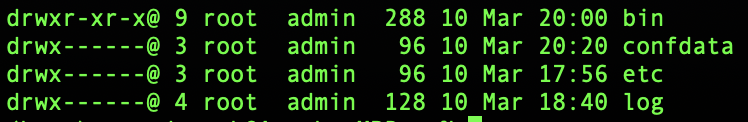
\includegraphics[width=0.48\linewidth]{img/lab-2/DIR_LAB2.png}
    \caption{Директории и права}
    \label{fig:dirlab2}
\end{figure}

Такие права были установлены так как: 
\begin{itemize}
    \item Логирование может читать только пользователь root (log/*.log);
    \item Хэшированные пароли, права, логины так же может видеть только root (etc/passwd);
    \item Исполняемые файлы пользователей (bin/*.sh)
    \item Исполняемые файлы владельца (bin/user\_manager.py, bin/config.py)
    \item Конфиденциальные данные доступны только авторизированные пользователям или root (confdata/*)
\end{itemize}

\subsubsection{Реализация выдачи доступа}

Основная логика выдачи доступа реализована в скрипте \texttt{access.py}, а учётные данные о пользователях и их правах хранятся в файле \texttt{/Users/practice2/etc/passwd}. Этот файл, а также журналы \texttt{/Users/practice2/log/access.log}, недоступны обычному пользователю (права \texttt{600}, владелец \texttt{root}), однако именно из них программа должна читать логины, хэшированные пароли и права, а также записывать события доступа. Поэтому при выдаче доступа нужно было одновременно обеспечить: невозможность прямого чтения/записи этих файлов пользователем и возможность контролируемого чтения/записи из \texttt{access.py} без использования \texttt{sudo}.

Логика выдачи доступа устроена следующим образом. Обычный пользователь запускает утилиту \texttt{run\_access}, которая на самом деле является небольшим setuid-бинарником на C (\texttt{run\_access.c}), установленным с владельцем \texttt{root} и битом SUID. Ядро запускает этот бинарник с эффективным идентификатором пользователя \texttt{EUID=root}, после чего он вызывает \texttt{/usr/bin/python3} с аргументом \texttt{/Users/practice2/bin/access.py}. Внутри \texttt{access.py} реализованы функции \texttt{elevate()}, \texttt{drop()} и \texttt{drop\_to\_real()}: при работе с файлом \texttt{passwd} и журналами выполняется временное повышение \texttt{EUID} до владельца файла (root), затем сразу же происходит возврат в контекст реального пользователя. Все проверки прав доступа к конфиденциальным файлам в каталоге \texttt{confdata/} выполняются уже с \texttt{EUID} обычного пользователя.

Скрипт \texttt{/Users/practice2/access.py} организует аутентификацию и выдачу прав следующим образом. В начале он импортирует модули \texttt{os}, \texttt{sys}, \texttt{getpass}, \texttt{hashlib}, \texttt{logging}, \texttt{shutil} и параметры из \texttt{config.py}. Модуль \texttt{os} используется для работы с файловой системой и идентификаторами пользователя: \texttt{os.stat()} (получение владельца файла \texttt{passwd}), \texttt{os.getuid()}/\texttt{os.geteuid()} (реальный и эффективный UID), \texttt{os.seteuid()} (временное повышение/понижение прав), \texttt{os.makedirs()} и \texttt{os.chmod()} (создание каталогов и установка прав доступа). Функции \texttt{read\_passwd()} и \texttt{write\_passwd()} оборачивают операции чтения/записи файла \texttt{passwd} в вызовы \texttt{elevate()/drop()}, а функция \texttt{\_setup\_logging()} аналогично открывает \texttt{access.log} под повышенными правами, после чего дальнейшая работа идёт уже от имени реального пользователя. Основной цикл команд (\texttt{read}, \texttt{append}, \texttt{copy}, \texttt{remove}, \texttt{perm}, \texttt{edit my info}) опирается исключительно на данные о правах из \texttt{passwd} и не требует root-доступа.

Попытка реализовать всё это только на Python оказалась невозможной в рамках требований macOS. Во-первых, установка бита SUID на самом \texttt{.py}-файле не даёт эффекта: ядро всё равно запускает интерпретатор \texttt{/usr/bin/python3} с правами вызывающего пользователя, а не владельца скрипта. Во-вторых, вызов \texttt{os.seteuid(0)} из процесса без привилегий запрещён - Python не может \guillemetleft сам по себе\guillemetright временно выдать себе \texttt{EUID} владельца файла. Поэтому была выбрана следующая схема: небольшой статически проверяемый бинарник на C, которому операционная система доверяет бит SUID, и уже из него - запуск Python-скрипта, который внутри умеет только понижать/поднимать \texttt{EUID} в допустимых границах.

Для удобства запуска поверх бинарника и Python-скриптов использованы небольшие shell-обёртки в каталоге \texttt{/Users/practice2/bin}. Они просто выполняют команду вида \texttt{exec /Users/practice2/bin/run\_access /Users/practice2/bin/access.py} (и для утилиты подбора пароля \texttt{crack.py}) с пробросом аргументов пользователя. Каталог \texttt{/Users/practice2/bin} добавляется в переменную окружения \texttt{PATH}, поэтому пользователь запускает утилиту короткой командой, без указания полного пути. Вся чувствительная часть (получение прав root и доступ к \texttt{etc/passwd} и \texttt{log/access.log}) реализована в небольшом C-бинарнике и в вызовах \texttt{os.seteuid()} внутри \texttt{access.py}, что и позволило корректно решить проблему выдачи доступа без использования \texttt{sudo} и без нарушения ограничений безопасности macOS.

\subsubsection{Реализация атаки brute force}

Для реализации атаки полного перебора был разработан скрипт \texttt{crack.py}, который читает хэш пароля целевого пользователя из файла \texttt{/Users/practice2/etc/passwd} и пытается восстановить исходный пароль по этому хэшу. Для хэширования паролей как в основной программе, так и в скрипте подбора используется алгоритм SHA256 из модуля \texttt{hashlib}, поэтому при генерации пробного пароля он сначала преобразуется в SHA256, а затем полученный дайджест побайтово сравнивается с сохранённым значением. Если хэши совпали, считается, что пароль найден, и утилита выводит найденный пароль, количество перебранных вариантов и затраченное время; если после перебора всех вариантов подходящей длины совпадения не было, выводится сообщение о неудаче и статистика по числу попыток и времени работы.

Для ограничения времени эксперимента введено жёсткое ограничение в 8 часов. В начале подбора фиксируется момент старта, а в цикле генерации паролей на каждой итерации проверяется текущее время; если с начала прошло больше 8 часов, перебор немедленно прерывается, и в выводе явно указывается, что подбор остановлен по таймауту, даже если пароль ещё не был найден. Это позволяет не \guillemetleft убить\guillemetright машину слишком долгим экспериментом при больших длинах пароля.

Число возможных паролей для заданной длины $L$ оценивается как
\[
N_L = 52 \cdot 72^{L-1},
\]
где 52 — количество допустимых символов для первой позиции (латинские буквы в верхнем и нижнем регистре), а 72 — количество возможных символов для каждой из последующих позиций (буквы, цифры и спецсимволы). Таким образом, первая буква всегда является буквой, а все остальные символы могут быть любыми из расширенного алфавита. Теоретическое суммарное количество вариантов от длины 1 до $L$ вычисляется как
\[
N_{\leq L} = \sum_{k=1}^{L} N_k,
\]
и именно это значение выводится режимом расчёта теоретической сложности.

Скрипт поддерживает два режима запуска. В основном режиме пользователь вызывает утилиту как \texttt{/Users/practice2/bin/run\_crack <LOGIN> <LENGTH>}, где \texttt{LOGIN} — имя пользователя, для которого выполняется подбор, а \texttt{LENGTH} — максимальная длина пароля. В этом случае сначала выводится теоретическое количество комбинаций и затем запускается реальный перебор с измерением времени. Во втором режиме, \texttt{/Users/practice2/bin/run\_crack -max-iterations <LENGTH>}, утилита не выполняет реальный перебор паролей, а только рассчитывает и выводит теоретическое число итераций и суммарное количество вариантов для длин от 1 до указанной, что позволяет оценить сложность атаки brute force без запуска длительного эксперимента.


\subsubsection{Реализация управления пользователями}

Управление пользователями в системе реализовано отдельной утилитой \texttt{/Users/practice2/bin/user\_manager.py}, представляющей собой Python-скрипт. Данная утилита предназначена только для администратора и запускается от имени \texttt{root}, так как работает напрямую с файлом \texttt{/Users/practice2/etc/passwd} и изменяет содержащиеся в нём записи. Обычный пользователь не имеет прав на запуск этой программы и на модификацию \texttt{passwd}.

Через \texttt{user\_manager.py} администратор может добавлять новых пользователей, редактировать уже существующих, изменять их основные данные (ФИО, идентификатор, хэш пароля) и присваивать или отзывать права доступа (на чтение, запись, удаление файлов в \texttt{confdata/}). Также поддерживается удаление пользователя: в этом случае соответствующая строка полностью убирается из \texttt{passwd}. Логика работы проста: при выборе операции утилита читает текущий файл \texttt{passwd}, находит (или создаёт) нужную запись по логину, вносит изменения в поля (пароль предварительно хэшируется тем же SHA256), после чего формирует новое содержимое и атомарно перезаписывает файл. Таким образом, все изменения прав и состава пользователей выполняются централизованно и контролируются только администратором.

\subsection{Примеры работы программы}
Ниже на рисунках \ref{fig:add_user} - \ref{fig:confdir}, представлены результаты работы программы:

На первом этапе через вход в суперпользователя, создаем пользователя New (см. рисунок \ref{fig:add_user}):

\begin{figure}[H]
    \centering
    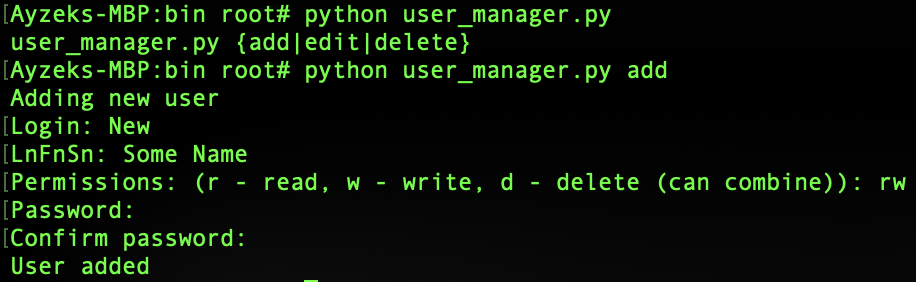
\includegraphics[width=0.48\linewidth]{img/lab-2/USER_ADD.png}
    \caption{Суперпользователь Root добавляет пользователя New}
    \label{fig:add_user}
\end{figure}

На рисунке \ref{fig:edit_user}, суперпользователь меняет данные о пользователе New: 

\begin{figure}[H]
    \centering
    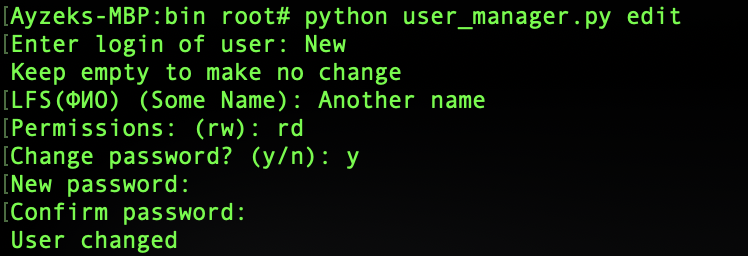
\includegraphics[width=0.48\linewidth]{img/lab-2/USER_EDIT.png}
    \caption{Суперпользователь Root меняет данные пользователя New}
    \label{fig:edit_user}
\end{figure}

После выхода через exit, можно попробывать авторизироватся через нового пользователя (рис. \ref{fig:autolab2}):

\begin{figure}[H]
    \centering
    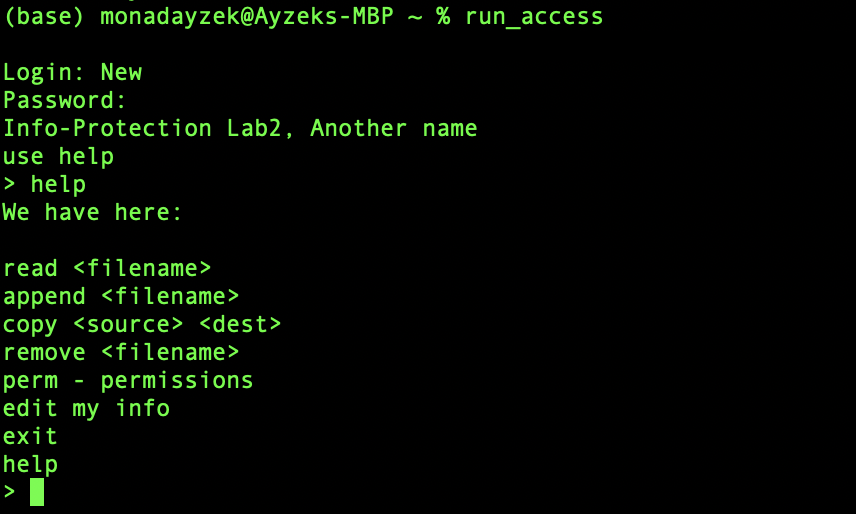
\includegraphics[width=0.48\linewidth]{img/lab-2/AUTO.png}
    \caption{Авторизация и пропись команды help}
    \label{fig:autolab2}
\end{figure}

Пользователь может прочесть файл или удалить, так как при изменении пользователя, суперпользователь дал права rd(\ref{fig:edit_user}), 
ниже на рисунке \ref{fig:read_delete} представлены действия пользователя по чтению и удалению файла:

\begin{figure}[H]
    \centering
    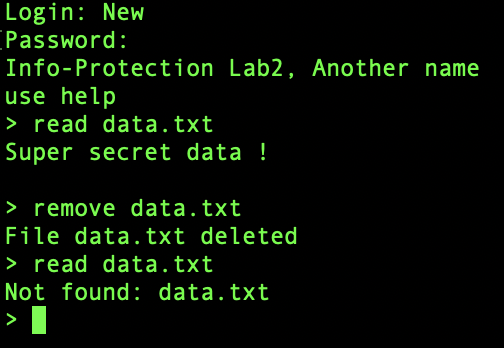
\includegraphics[width=0.48\linewidth]{img/lab-2/READ_DEL.png}
    \caption{Чтение и удаление файла пользователем с правами rw}
    \label{fig:read_delete}
\end{figure}

Далее на рисуке \ref{fig:passwdlab2}, представлена структура хранения хэшей согласно требованиям:

\begin{figure}[H]
    \centering
    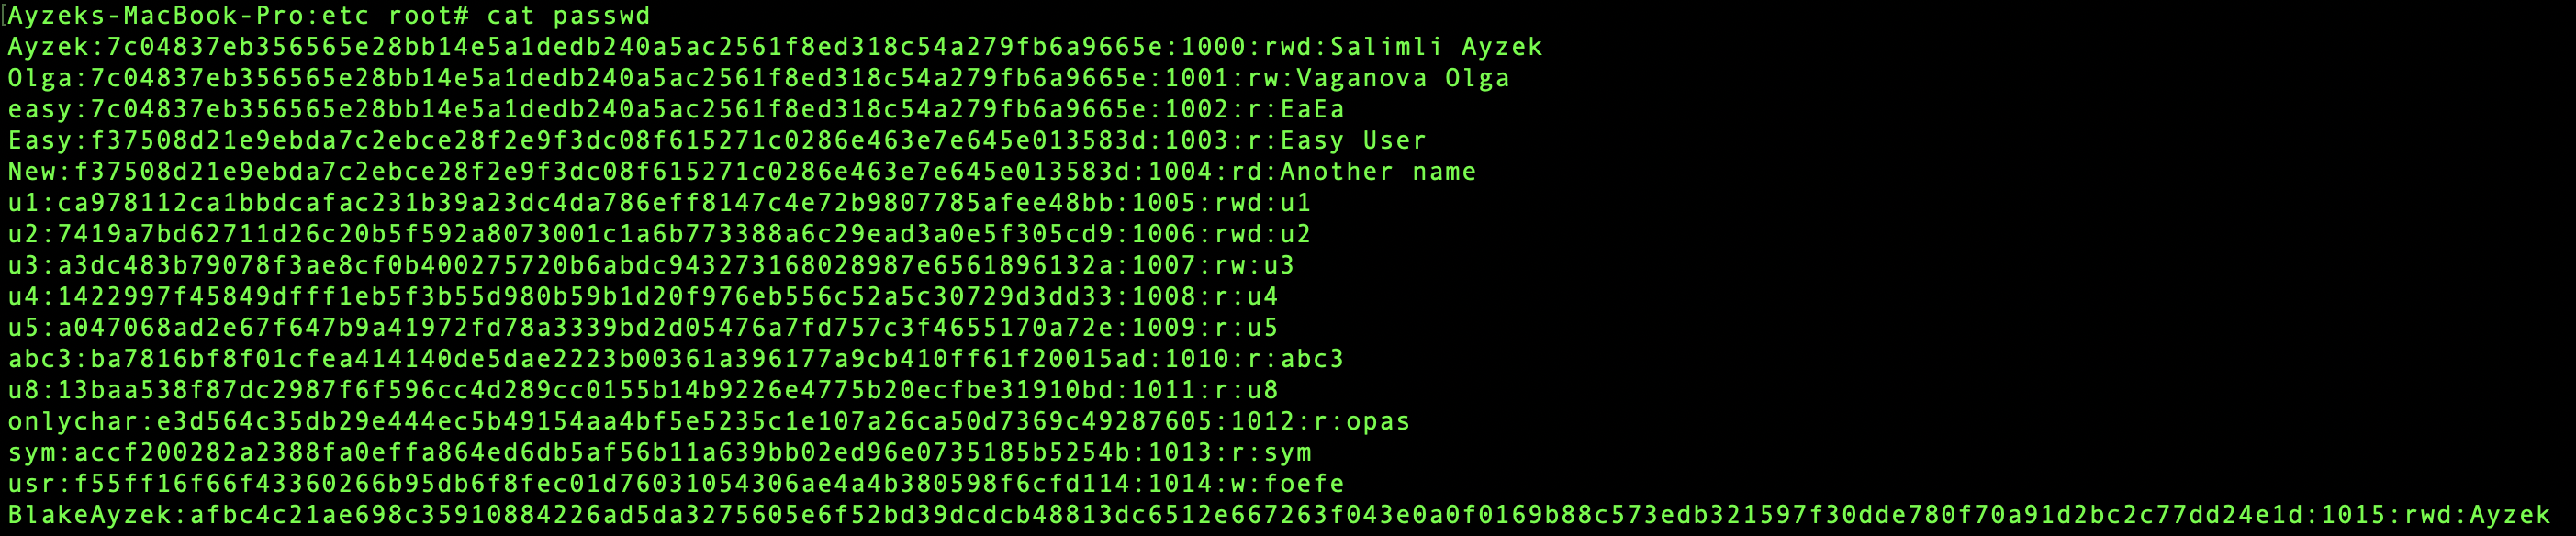
\includegraphics[width=0.48\linewidth]{img/lab-2/PASSWD.png}
    \caption{Хранение данных в passwd}
    \label{fig:passwdlab2}
\end{figure}

Как видно, структура хранения имеет вид - Логин:Хэш-значение:UID:Права:ФИО.

Ниже показан вывод логирования, на рисунке \ref{fig:accesslog} представлено логирование действий, а на рисунке \ref{fig:authlog} - логирование авторизаций:

\begin{figure}[H]
    \centering
    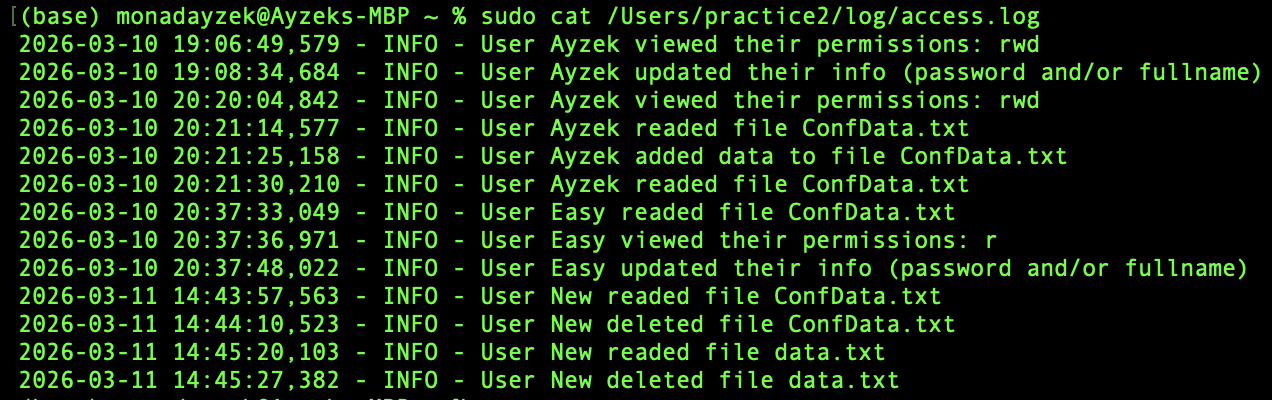
\includegraphics[width=0.48\linewidth]{img/lab-2/ACCESSLOG.png}
    \caption{Логирование действий пользователей}
    \label{fig:accesslog}
\end{figure}

\begin{figure}[H]
    \centering
    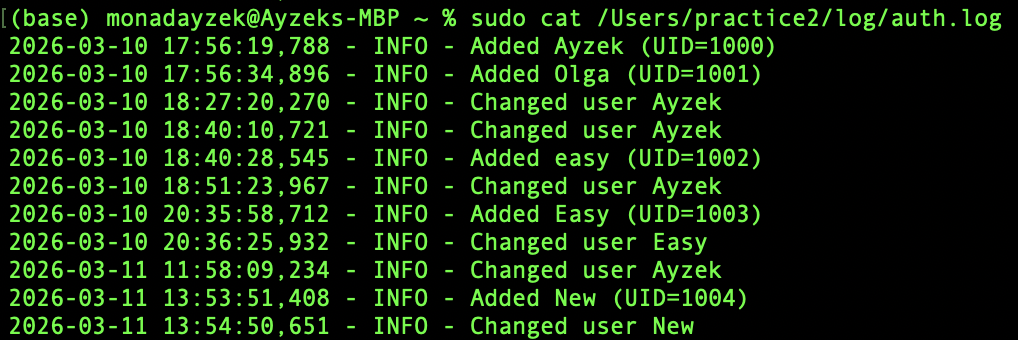
\includegraphics[width=0.48\linewidth]{img/lab-2/AUTHLOG.png}
    \caption{Логирование действий авторизации}
    \label{fig:authlog}
\end{figure}

В каталоге confdata, находятся обычные текстовые файлы, которые были созданы суперпользователем путем VIM (или др. редактором):

\begin{figure}[H]
    \centering
    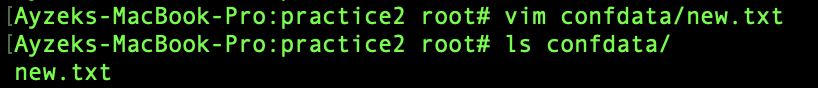
\includegraphics[width=0.48\linewidth]{img/lab-2/CONFDIR.png}
    \caption{Каталог confdata}
    \label{fig:confdir}
\end{figure}

\subsection{Атака brute force}

Для исследования зависимости итераций и времени на нахождения пароля, было создано 9 пользователей со следующими атрибутами пароля:

\begin{itemize}
    \item u1 : $L = 1, p \in \mathbb{C} \cup \mathbb{N}$
    \item u2 : $L = 2, p \in \mathbb{C} \cup \mathbb{N}$
    \item u3 : $L = 2, p \in \mathbb{C} \cup \mathbb{N}$
    \item u4 : $L = 2, p \in \mathbb{C} \cup \mathbb{N}$
    \item u5 : $L = 2, p \in \mathbb{C} \cup \mathbb{N}$
    \item onlychar : $L = 4, p \in \mathbb{L}$
    \item abc3 : $L = 3, p = abc$
    \item sym : $L = 4, p \in \mathbb{C} / \mathbb{L}$
    \item u8 : $L = 8, p \in (\mathbb{C} / \mathbb{L}) \cup \mathbb{N},$
\end{itemize}
где $L$ - длина пароля, $p$ - значение пароля, $\mathbb{C}$ - множество символов и букв, $\mathbb{N}$ - натуральные числа включая 0, $\mathbb{L}$ - множество букв.

Графики результатов разделены на 2 части: по длинам пароля, по значениям пароля и по длине = 8.

Резульаты проведения эксперимента представленны на рисунке \ref{fig:res_brute} для длин пароля и на рисунке \ref{fig:res_brute_value} для значений пароля.

\begin{figure}[H]
    \centering
    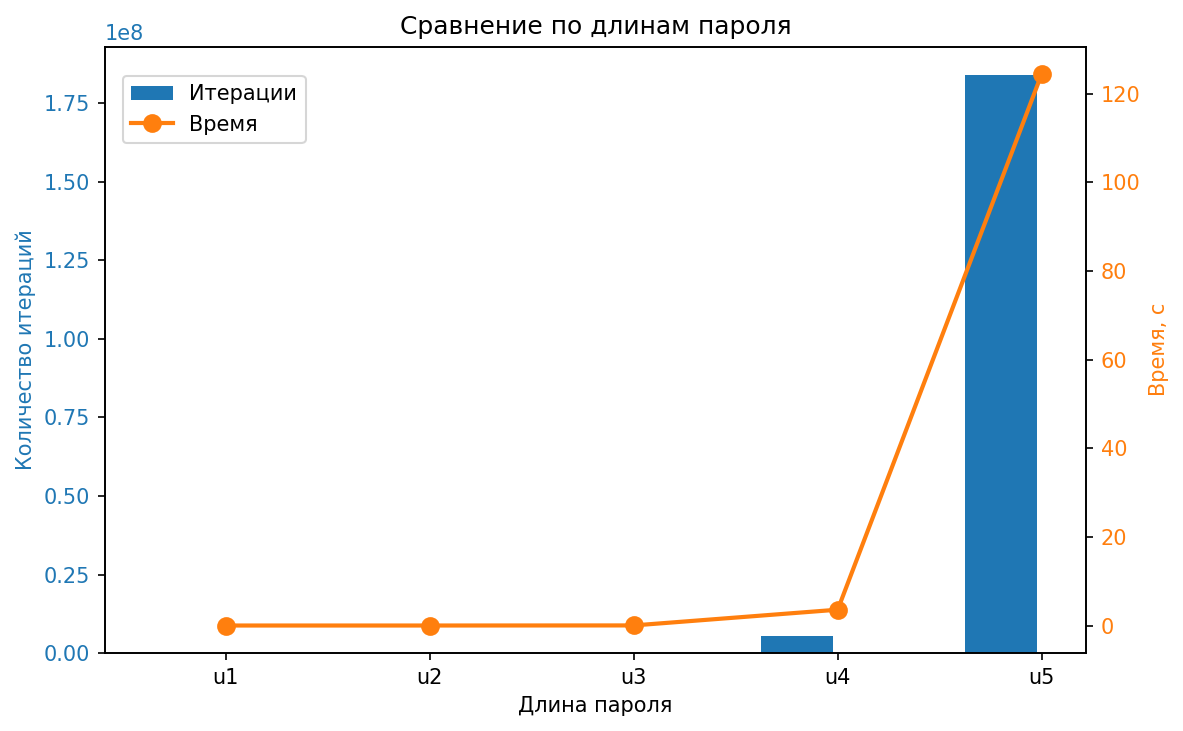
\includegraphics[width=0.48\linewidth]{img/lab-2/RES_BRUTE.png}
    \caption{Результаты проведения эксперимента для длин пароля}
    \label{fig:res_brute}
\end{figure}

\begin{figure}[H]
    \centering
    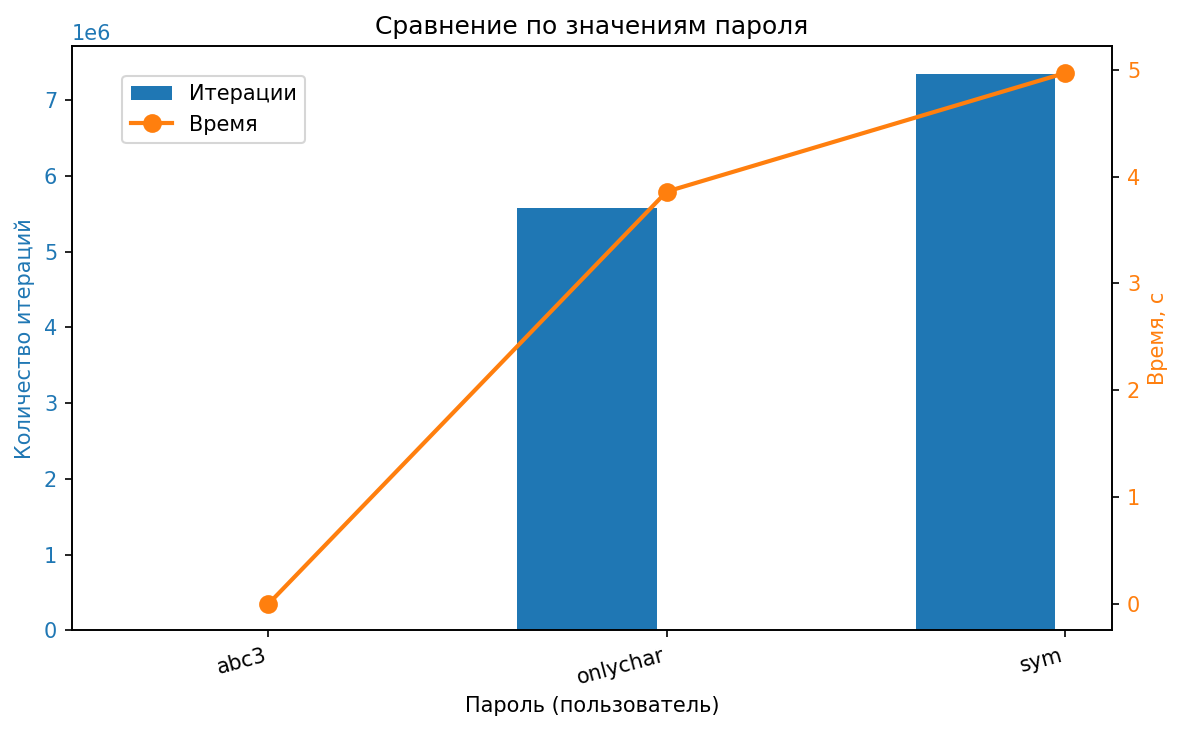
\includegraphics[width=0.48\linewidth]{img/lab-2/RES_BRUTE_VALUE.png}
    \caption{Результаты проведения эксперимента для значений пароля}
    \label{fig:res_brute_value}
\end{figure}

Как видно при увеличеинии длины пароля, количество итераций и времени на нахождения пароля увеличивается экспоненциально.

Для пользователя u8, было подсчитано:
$$
    \frac{N_8}{N_5} = \frac{52 \cdot 72^{8-1}}{52 \cdot 72^{5-1}} = 72^3 = 373248.
$$
То есть для нахождения пароля длиной 8, нужно в 373248 раз больше итераций, чем для пароля длиной 5.
Для нахождения пароля длиной 5 заняло 124.40 секунд, тогда для нахождения пароля длиной 8 заняло бы явно больше 8 часов. В коде сработал бы таймаут. 

\subsection*{Заключение}
\addcontentsline{toc}{subsection}{Заключение}

В ходе лабораторной работы была реализована и исследована простая система управления доступом к конфиденциальным данным. Для этого были спроектированы отдельные каталоги \texttt{/Users/practice2} и \texttt{/Users/practice3} с жёстко заданными правами, реализованы утилиты аутентификации и доступа (\texttt{access.py}), подбора паролей (\texttt{crack.py}) и административного управления пользователями (\texttt{user\_manager.py}). Для корректной работы с защищёнными файлами \texttt{etc/passwd} и журналами при сохранении ограничений macOS был использован setuid-бинарник на C и аккуратное управление эффективным идентификатором пользователя из Python-кода.

Также были реализованы и протестированы модели дискреционного и мандатного управления доступом (DAC и MAC) с использованием тех же принципов хранения и проверки прав. В рамках экспериментов исследована сложность атаки brute force для различных длин паролей и сопоставлены теоретические оценки с практическими результатами. В целом поставленные в работе задачи по проектированию и реализации защищённого доступа к файлам, организации хранения служебных данных и моделированию атак были выполнены.

Исходные коды практической работы №2, доступны в приложении \hyperref[sec:pril2]{А}, где:
\begin{itemize}
    \item access.py - скрипт авторизации пользователя;
    \item run\_access.c - утилита для подготовки исполняемого кода;
    \item run\_access - shell-скрипт для исполнения скрипта авторизации пользователя с выдачей EUID;
    \item crack.py - скрипт для атаки brute force;
    \item user\_manager.py - скрипт для управления пользователями (chmod 700); 
    \item config.py - скрипт задающий конфигурацию основным утилитам. 
\end{itemize}

% разработке, применяемых языках программирования;
% − сведения об используемом алгоритме хэширования;
% − примеры компиляции и сборки приложений (если используется
% компилируемый язык);
% − примеры запуска и работы утилит;
% − пример расчета максимального количества итераций и времени
% взлома для заданной длины пароля;
% − результаты исследования в виде таблицы или графика:
% 4
% Зашита информации, 2026
% o рассчитанное максимальное количество итераций и время взлома
% для указанных длин паролей;
% o полученное в результате экспериментов количество итераций и
% время взлома для указанных длин паролей.
% − выводы по проделанной работе.

\newpage
\section{Реализация моделей дискреционного и мандатного управления доступом}
\subsection{Введение}

Помимо базовой аутентификации и разграничения прав по субъектам, в защищённых системах применяют модели дискреционного (DAC) и мандатного (MAC) управления доступом. Дискреционная модель позволяет владельцу объекта самостоятельно назначать и отзывать права доступа другим субъектам; таким образом реализуется гибкое управление доступом на уровне файлов и пользователей. Мандатная модель опирается на метки конфиденциальности субъектов и объектов: доступ разрешён только при соблюдении правил (например, \guillemetleft не читать выше своего уровня\guillemetright, \guillemetleft не записывать ниже\guillemetright), что снижает риск утечки при компрометации учётной записи. В данной главе кратко описывается реализация обеих моделей в рамках лабораторного стенда и их связь с утилитами доступа к конфиденциальным данным.

\subsection{Постановка задачи}

\subsubsection{Цели}
\begin{itemize}
    \item изучить особенности моделей дискреционного (DAC) и мандатного (MAC) управления доступом;
    \item на базе разработанной в практической работе 2 системы аутентификации и авторизации реализовать DAC и MAC.
\end{itemize}
\subsubsection{Задачи}
\begin{itemize}
    \item На базе разработанной в практической работе 2 системы аутентификации
    и авторизации разработать систему, реализующую DAC, включая: \begin{itemize}
        \item владение объектами;
        \item произвольное назначение прав доступа к объекту;
        \item контроль на основе матрицы или списка доступа.
        \end{itemize}
    \item На базе разработанной в практической работе 2 системы аутентификации
    и авторизации разработать систему, реализующую MAC, включая: \begin{itemize}
        \item метки безопасности для субъектов и объектов;
        \item свойства безопасности модели Белла-Лападулы.
        \end{itemize}
\end{itemize}

\subsection{Требования к работе}
\begin{itemize}
    \item Требования к дереву каталогов, остается прежним, однако создается новая родительская директория practice3;
    \item Требования к DAC: \begin{itemize}
        \item у каждого объекта должен быть владелец, который может
        произвольно назначать и передавать права доступа к этому объекту;
        \item контроль доступа к объектам должен осуществляться на основе
        матрицы или списка доступа, в которых хранится информация о правах
        доступа субъектов к объектам.
        \end{itemize}
    \item Требования к MAC: \begin{itemize}
        \item каждому субъекту и объекту должна присваиваться метка
        безопасности суперпользователем;
        \item предусмотреть не менее трех уровней меток безопасности: \guillemetleft несекретно\guillemetright, \guillemetleft для служебного пользования (ДСП)\guillemetright, \guillemetleft секретно\guillemetright;
        \item субъекты не могут менять метки безопасности;
        \item контроль доступа к объектам должен осуществляться на основе свойств безопасности модели Белла-Лападулы: \guillemetleft нет чтения сверху\guillemetright, \guillemetleft нет записи вниз\guillemetright и дискреционного свойства.
        \end{itemize}
\end{itemize}

\subsection{Сведения о DAC и MAC}
\subsubsection{DAC (Discretionary Access Control)}
Дискреционное управление доступом (DAC) — модель разграничения доступа, в которой владелец ресурса самостоятельно определяет права субъектов на объекты (чтение, запись, исполнение). Права фиксируются в матрице доступа или списках ACL. Особенность: гибкость управления при потенциальной уязвимости к несанкционированной передаче прав.

\subsubsection{MAC (Mandatory Access Control)}
Мандатное управление доступом (MAC) — модель, основанная на присвоении меток безопасности субъектам и объектам. Доступ разрешается только при выполнении правил сравнения меток, централизованно заданных политикой безопасности. Ключевой принцип реализуется моделью Белла-Лападулы, обеспечивающей иерархический контроль потоков информации и предотвращающей несанкционированное понижение уровня конфиденциальности. В отличие от DAC, пользователь не может изменять политику доступа.

\subsection{Реализация DAC}

Реализация дискреционной модели выполнена поверх предыдущей практической работы: используется тот же принцип аутентификации по \texttt{/Users/practice3/etc/passwd}, те же утилиты доступа и логирования. Все файлы системы размещены в \texttt{/Users/practice3/} (каталоги \texttt{etc}, \texttt{confdata}, \texttt{bin}, \texttt{log}). Такое построение добавляет дополнительный уровень разграничения доступа и способствует обеспечению конфиденциальности, целостности и доступности информации: владелец файла явно задаёт, кто имеет право читать, изменять или удалять его данные, а все действия фиксируются в логах.

Владение реализовано так: при создании файла командой \texttt{create} пользователь, создавший файл, записывается как владелец (\texttt{owner}) этого объекта. Создаётся запись в служебном хранилище, и владельцу сразу выдаются полные права \texttt{rwd} на созданный файл. Передача прав выполняется командами \texttt{grant} и \texttt{revoke}. Выдать права (\texttt{grant <файл> <пользователь> <права>}) может только владелец файла; отозвать права (\texttt{revoke <файл> <пользователь>}) также может только владелец. Нельзя отозвать права у самого себя (владелец остаётся единственным, кто может управлять списком доступа). Проверка при операциях чтения, записи и удаления: у субъекта должна быть соответствующая буква (\texttt{r}, \texttt{w} или \texttt{d}) в его записи для данного файла.

Информация о доступе хранится не в виде одной матрицы «субъект-объект», а по объектам: для каждого файла ведётся свой список прав. Список доступа (ACL, Access Control List) — это перечень пар «субъект : права» для одного объекта. В нашей реализации ACL хранится в файле \texttt{/Users/practice3/etc/acl.json} в формате JSON: для каждого имени файла задаётся поле \texttt{owner} (логин владельца) и поле \texttt{acl} — словарь вида \texttt{\{ "логин": "rwd", ... \}}. Таким образом, матрица доступа представлена в виде набора ACL по файлам, что эквивалентно хранению по столбцам матрицы доступа.

\subsection{Реализация MAC}

Реализация мандатной модели также выполнена поверх той же базы: каталог \texttt{/Users/practice3/}, общий \texttt{passwd} и общая структура утилит доступа. В \texttt{passwd} для каждого пользователя хранится не только логин, хэш пароля и права, но и уровень конфиденциальности (метка субъекта). Используются три уровня: 0 — unclassified, 1 — DSP, 2 — secret. Метки объектов (файлов) хранятся отдельно в \texttt{/Users/practice3/etc/file\_labels.json}: для каждого имени файла записан числовой уровень (0, 1 или 2). При создании файла командой \texttt{create} файлу присваивается метка, равная уровню создателя; таким образом, метка объекта задаётся один раз при создании и в дальнейшем определяет, кто может читать или записывать этот объект по правилам Белла-Лападулы.

Доступ по чтению разрешён только если уровень субъекта не ниже уровня объекта (No Read Up): пользователь с уровнем 0 не может читать файлы с уровнем 1 или 2; с уровнем 1 — не может читать уровень 2. Доступ по записи разрешён только если уровень субъекта не выше уровня объекта (No Write Down): пользователь с уровнем 2 не может записывать в файлы с уровнем 1 или 0, чтобы не понижать конфиденциальность данных. В коде это реализовано функциями \texttt{check\_mac\_read} (разрешение при \texttt{subject\_level >= object\_level}) и \texttt{check\_mac\_write} (разрешение при \texttt{subject\_level <= object\_level}). Перед каждой операцией чтения или записи выполняется соответствующая проверка; при нарушении выводится сообщение об отказе с указанием уровней. Удаление файла по-прежнему контролируется дискреционным ACL: право \texttt{d} у субъекта на данный объект и владение; при этом при создании и удалении обновляется и \texttt{file\_labels.json}.

Список доступа (ACL) в MAC хранится так же, как в DAC: в \texttt{/Users/practice3/etc/acl.json} — владелец и права \texttt{rwd} по пользователям для каждого файла. Дополнительно в \texttt{/Users/practice3/etc/file\_labels.json} хранится метка конфиденциальности каждого файла. Итоговое решение доступа: сначала проверяется DAC (есть ли у пользователя нужное право в ACL), затем MAC (соблюдаются ли правила No Read Up и No Write Down по меткам). Таким образом, мандатная политика накладывается поверх дискреционной и обеспечивает запрет недопустимых потоков информации по уровням.

\subsection{Примеры работы программы}
Ниже на рисунках \ref{fig:dac_user}-\ref{fig:dac_matrix}, представлен пример работы программы с контролем доступа DAC:

\begin{figure}[H]
    \centering
    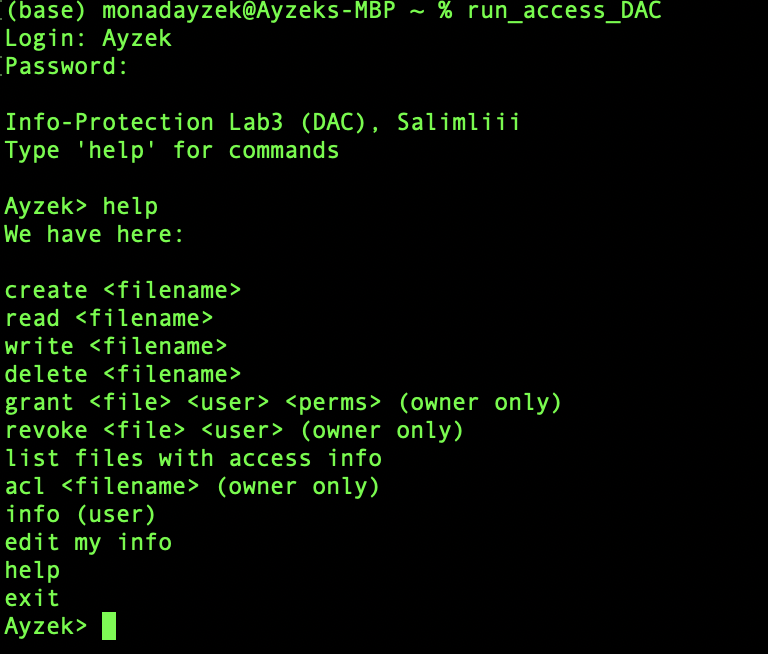
\includegraphics[width=0.48\linewidth]{img/lab-3/DAC_USER.png}
    \caption{Пользователь Ayzek вызвал инструкцию help}
    \label{fig:dac_user}
\end{figure}

Создание файла пользователем, автоматически назначает пользователя владельцем файла дав права rwd (рис. \ref{fig:dac_create}):

\begin{figure}[H]
    \centering
    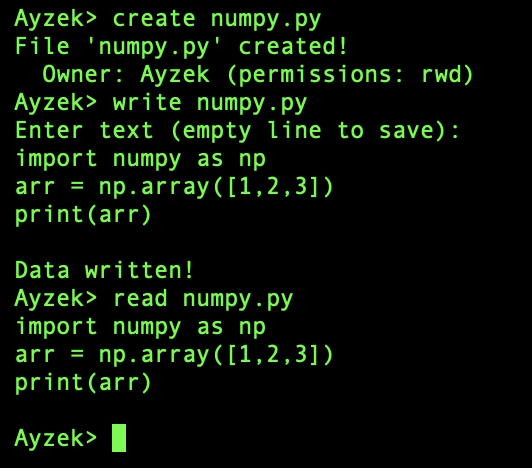
\includegraphics[width=0.48\linewidth]{img/lab-3/DAC_CREATE.png}
    \caption{Пользователь Ayzek создал файл numpy.py}
    \label{fig:dac_create}
\end{figure}

Владелец файла может передать право другому пользователю (рис. \ref{fig:dac_grant}):

\begin{figure}[H]
    \centering
    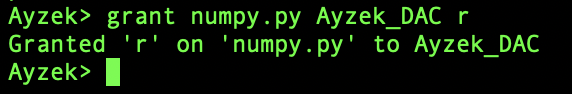
\includegraphics[width=0.48\linewidth]{img/lab-3/DAC_GRANT.png}
    \caption{Пользователь Ayzek передал право на файл numpy.py пользователю Ayzek\_DAC}
    \label{fig:dac_grant}
\end{figure}

Переключившись на пользователя Ayzek\_DAC, мы можем проверить, что он может читать файл numpy.py и не может записывать или удалять его (рис. \ref{fig:dac_perm}):

\begin{figure}[H]
    \centering
    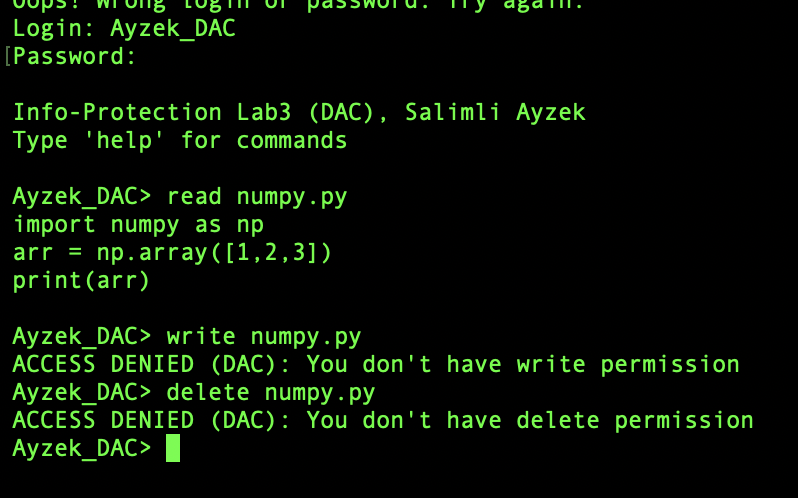
\includegraphics[width=0.48\linewidth]{img/lab-3/DAC_PERM.png}
    \caption{Пользователь Ayzek\_DAC может читать файл numpy.py и не может записывать или удалять его}
    \label{fig:dac_perm}
\end{figure}

Ниже на рисунке \ref{fig:dac_list}, представлен простой лист прав и владельцев, файлов и прав на них:

\begin{figure}[H]
    \centering
    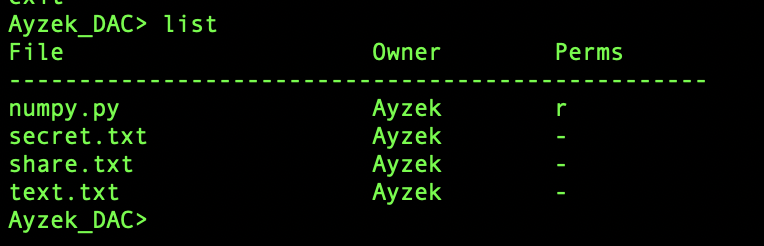
\includegraphics[width=0.48\linewidth]{img/lab-3/DAC_LIST.png}
    \caption{Лист прав и владельцев, файлов и прав на них}
    \label{fig:dac_list}
\end{figure}

Владелец файла может увидеть ACL для файла numpy.py (рис. \ref{fig:dac_acl}):

\begin{figure}[H]
    \centering
    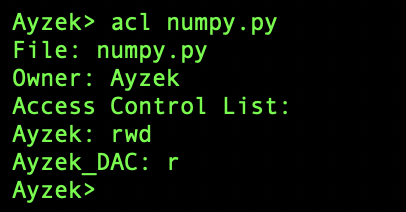
\includegraphics[width=0.48\linewidth]{img/lab-3/DAC_ACL.png}
    \caption{ACL для файла numpy.py}
    \label{fig:dac_acl}
\end{figure}

Далее на рисунках \ref{fig:dac_passwd} и \ref{fig:dac_acl_json}, представлен содержимое файлов passwd и acl.json для DAC:

\begin{figure}[H]
    \centering
    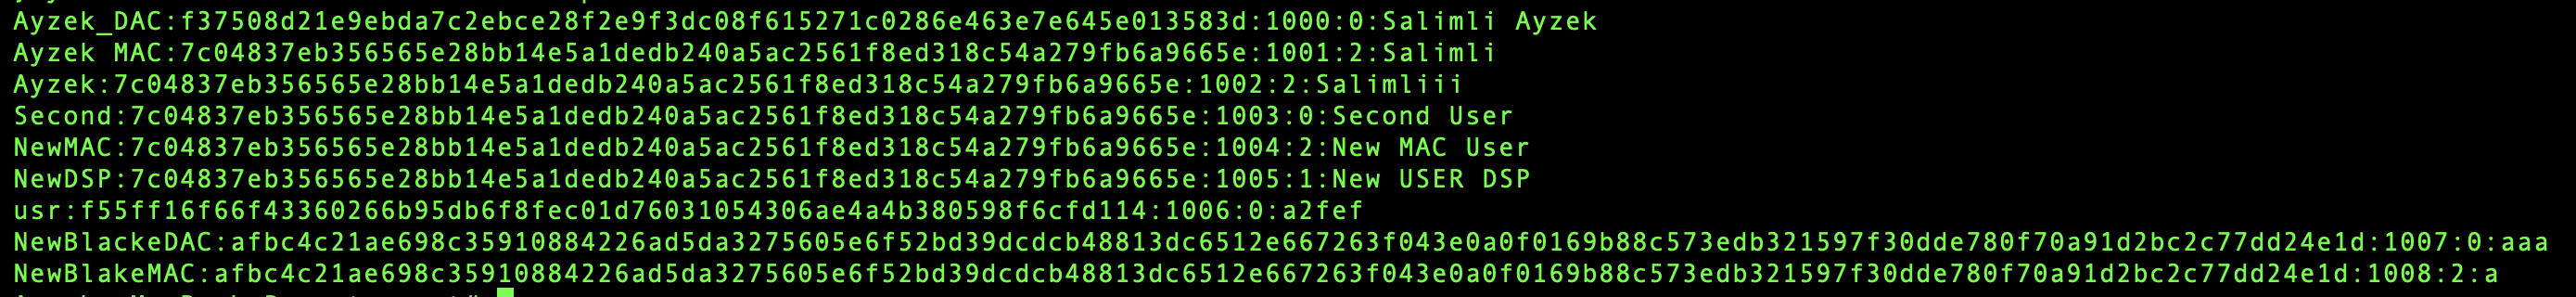
\includegraphics[width=0.48\linewidth]{img/lab-3/DAC_PASSWD.png}
    \caption{Содержимое файла passwd для DAC}
    \label{fig:dac_passwd}
\end{figure}

\begin{figure}[H]
    \centering
    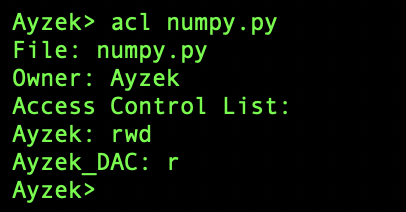
\includegraphics[width=0.48\linewidth]{img/lab-3/DAC_ACL.png}
    \caption{Содержимое файла acl.json для DAC}
    \label{fig:dac_acl_json}    
\end{figure}

Так как реализация MAC и DAC имеют единный каталог, на рисунке \ref{fig:dac_passwd}, видны цифры от 0 до 2, которые обозначают уровень конфиденциальности субъекта и объекта.
Но они не имеют отношения к DAC, так как данные о правах берутся из файла acl.json, а пароль и логин из passwd.

Ниже представлена матрица доступа для DAC (рис. \ref{fig:dac_matrix}):

\begin{figure}[H]
    \centering
    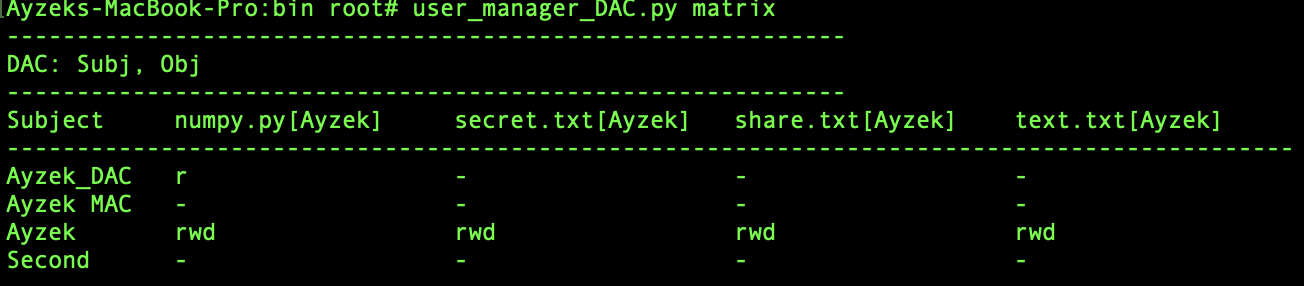
\includegraphics[width=0.48\linewidth]{img/lab-3/DAC_MATRIX.png}
    \caption{Матрица доступа для DAC}
    \label{fig:dac_matrix}
\end{figure}

Матрица предствляет собой субъекты, объекты и права между ними.

Далее на рисунках \ref{fig:mac_add_user}-\ref{fig:mac_matrix}, представлен пример работы программы с контролем доступа MAC:

Ниже добавление пользователя с указанием уровня конфиденциальности (рис. \ref{fig:mac_add_user}):

\begin{figure}[H]
    \centering
    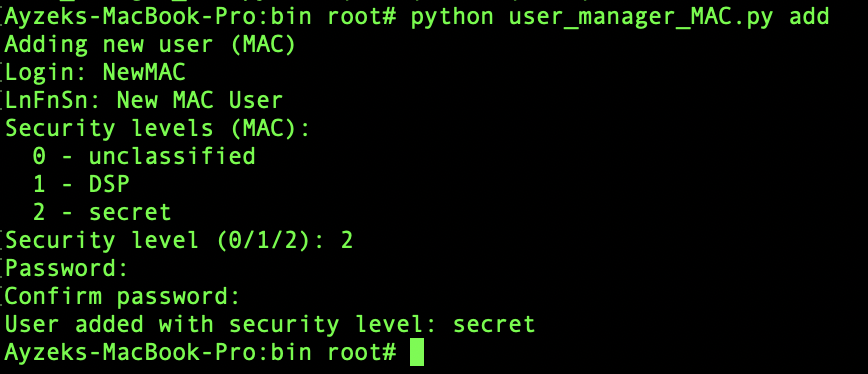
\includegraphics[width=0.48\linewidth]{img/lab-3/MAC_USER.png}
    \caption{Добавление пользователя с указанием уровня конфиденциальности}
    \label{fig:mac_add_user}
\end{figure}

По правилам, пользователь NewMAC, может создать файл только с уровнем конфиденциальности 2 (secret) (рис. \ref{fig:mac_create}):

\begin{figure}[H]
    \centering
    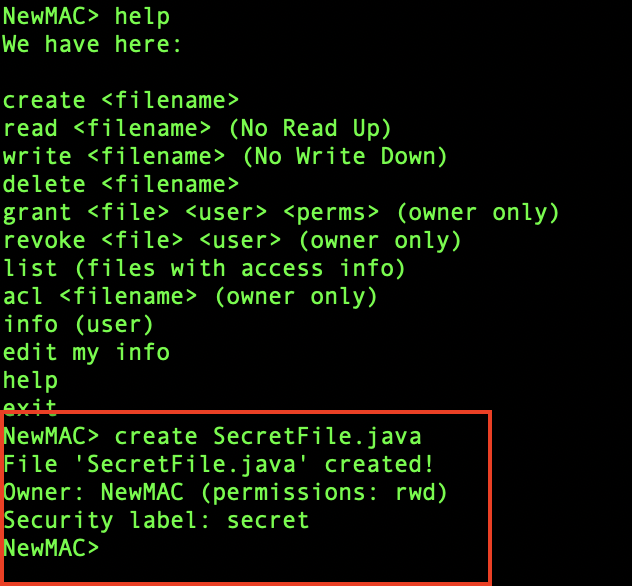
\includegraphics[width=0.48\linewidth]{img/lab-3/MAC_CREATE.png}
    \caption{Создание файла с уровнем конфиденциальности 2 (secret)}
    \label{fig:mac_create}
\end{figure}

Теперь можно создать пользователя с уровнем конфиденциальности 1 (ДСП) (рис. \ref{fig:mac_add_user_dsp}):

\begin{figure}[H]
    \centering
    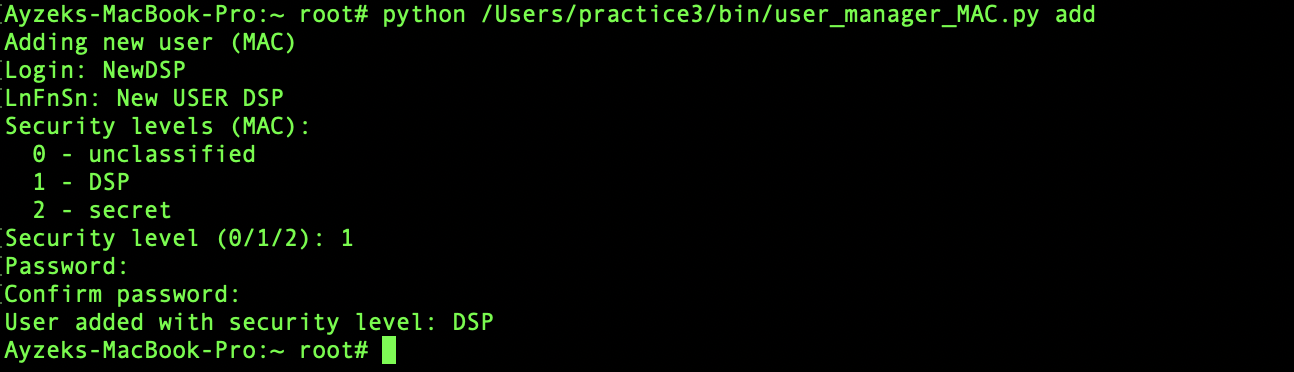
\includegraphics[width=0.48\linewidth]{img/lab-3/MAC_USER_DSP.png}
    \caption{Добавление пользователя с уровнем конфиденциальности 1 (ДСП)}
    \label{fig:mac_add_user_dsp}
\end{figure}

Пользователь NewDSP, может создать файл только с уровнем конфиденциальности 1 (ДСП) (рис. \ref{fig:mac_create_dsp}):

\begin{figure}[H]
    \centering
    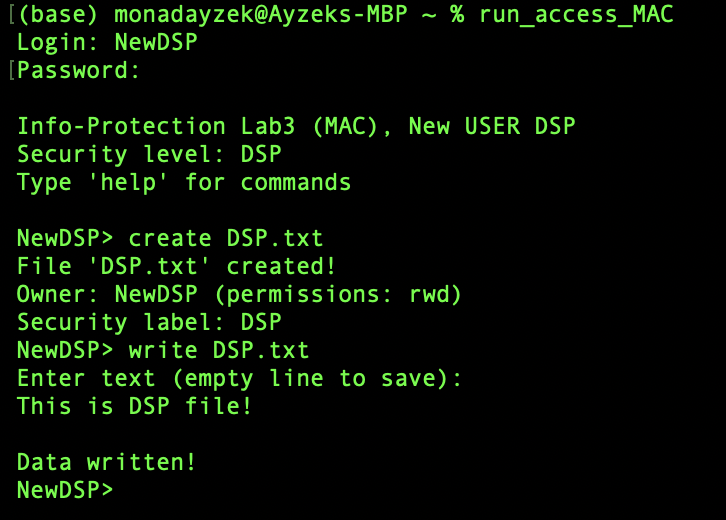
\includegraphics[width=0.48\linewidth]{img/lab-3/MAC_CREATE_DSP.png}
    \caption{Создание файла с уровнем конфиденциальности 1 (ДСП)}
    \label{fig:mac_create_dsp}
\end{figure}

По правилу Белла-Лападулы, пользователь NewDSP не может читать файлы с уровнем конфиденциальности 2 (secret), 
а пользователь NewMAC может читать файлы с уровнем конфиденциальности 1 (ДСП) и 2 (secret), но не может записывать в них как показано на рисунке \ref{fig:rule_mac}:

\begin{figure}[H]
    \centering
    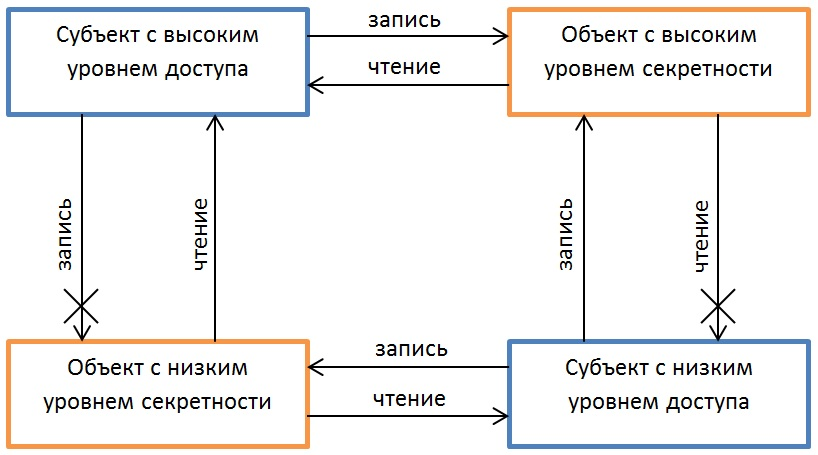
\includegraphics[width=0.48\linewidth]{img/lab-3/RULE_MAC.png}
    \caption{Правило Белла-Лападулы}
    \label{fig:rule_mac}
\end{figure}

Далее на рисунке \ref{fig:mac_test}, показан сценарий попытки чтения файла SecretFile.java, пользователем NewDSP, а на рисунке 
\ref{fig:mac_test_2}, показан сценарий попытки записи в файл DSP.txt пользователем NewMAC. Для проведения сценария сначала нужно дать права друг другу на чтение и запись.

\begin{figure}[H]
    \centering
    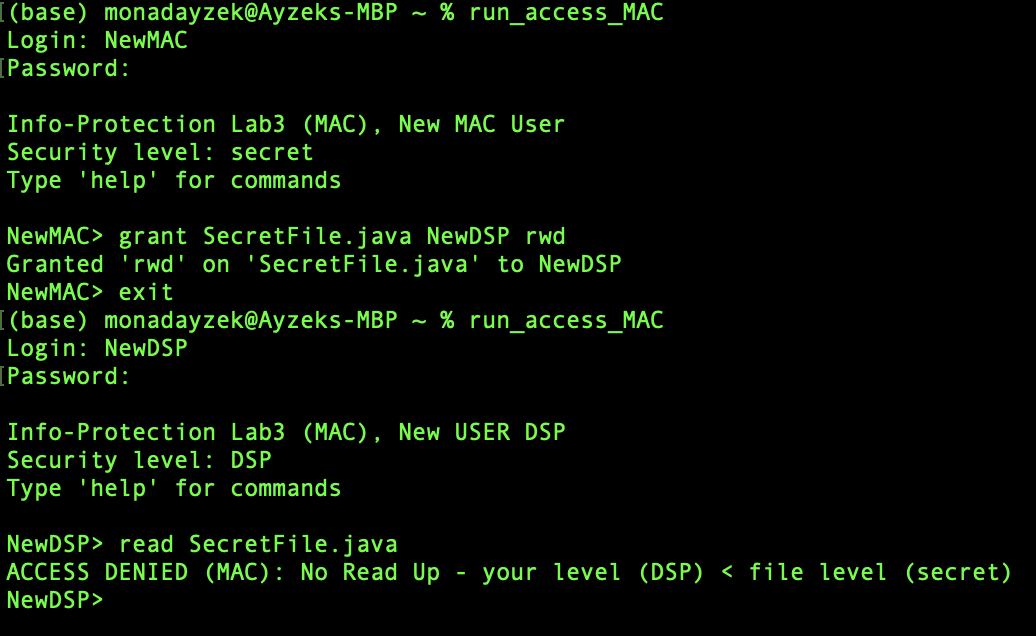
\includegraphics[width=0.48\linewidth]{img/lab-3/MAC_TEST_2.png}
    \caption{Сценарий попытки чтения файла SecretFile.java, пользователем NewDSP}
    \label{fig:mac_test}
\end{figure}

\begin{figure}[H]
    \centering
    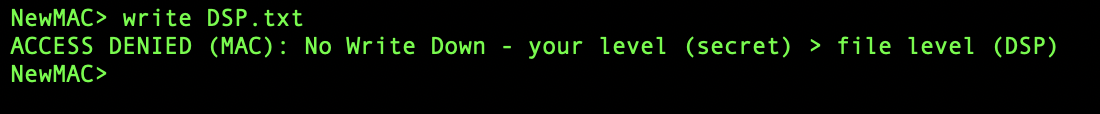
\includegraphics[width=0.60\linewidth]{img/lab-3/MAC_TEST.png}
    \caption{Сценарий попытки записи в файл DSP.txt пользователем NewMAC}
    \label{fig:mac_test_2}
\end{figure}

Как видно из рисунка \ref{fig:mac_test}, если не дать права друг другу, то ошибка, будет касатся DAC контроля доступа (нет права).

Ниже на рисунке \ref{fig:mac_matrix}, представлена матрица доступа для MAC:

\begin{figure}[H]
    \centering
    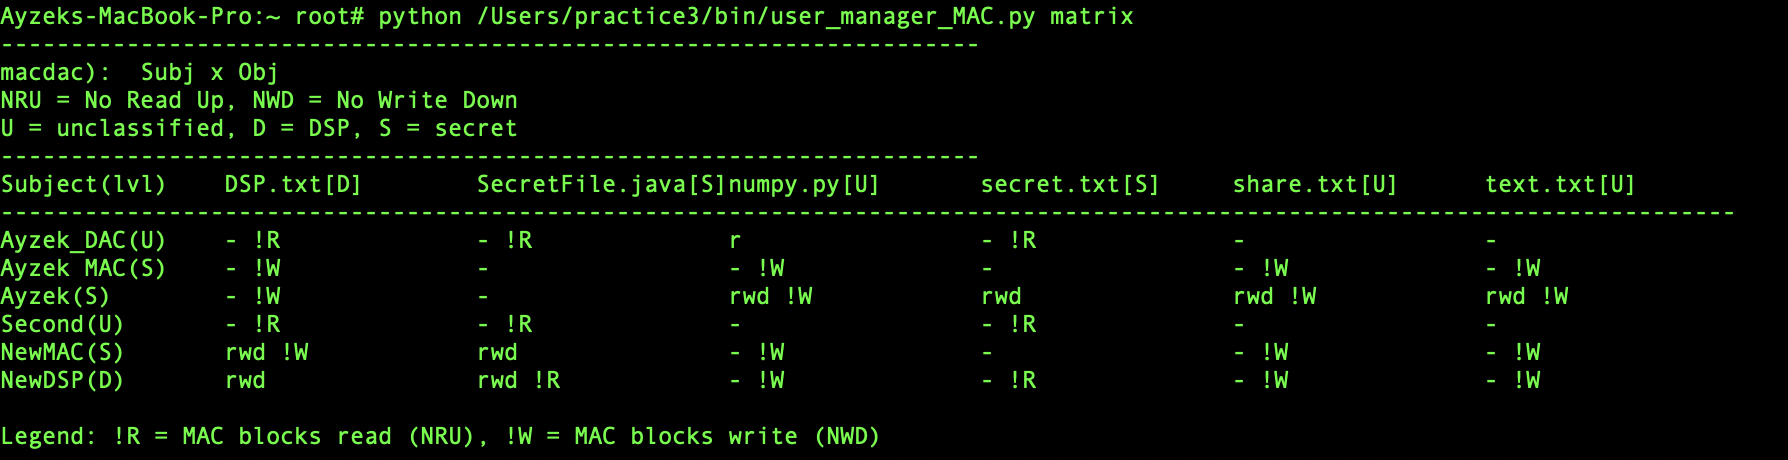
\includegraphics[width=0.60\linewidth]{img/lab-3/MAC_MATRIX.png}
    \caption{Матрица доступа для MAC}
    \label{fig:mac_matrix}
\end{figure}

Ниже матрицы указана легенда: !R - блокировка чтения, !W - блокировка записи, так же рядом указаны права доступа.
Символы (U,D,S) обозначают уровень конфиденциальности субъекта и объекта.

\subsection{Атака brute force}

Атака не влияет на выбор метода аутентификации, так как пароль хэшируется перед сохранением в файл.

Ниже в таблице \ref{tab:res_brute}, продублированы результаты проведения эксперимента для всех паролей:

\begin{table}[H]
    \centering
    \caption{Результаты проведения эксперимента для всех паролей}
    \label{tab:res_brute}
    \begin{tabular}{|c|c|c|}
        \hline
        \textbf{Пользователь} & \textbf{Количество итераций} & \textbf{Время, с} \\
        \hline
        \texttt{u1}      & 1         & 0.00  \\
        \texttt{u2}      & 478       & 0.00  \\
        \texttt{u3}      & 24095     & 0.02  \\
        \texttt{u4}      & 5414807   & 3.57  \\
        \texttt{u5}      & 183837715 & 124.40 \\
        \texttt{abc3}    & 3871      & 0.00  \\
        \texttt{onlychar}& 5576615   & 3.86  \\
        \texttt{sym}     & 7338865   & 4.97  \\
        \texttt{u8}      & -        & Начался SWAP \\
        \hline
    \end{tabular}
\end{table}


\subsection*{Заключение}
\addcontentsline{toc}{subsection}{Заключение}

В данной главе были реализованы и исследованы модели дискреционного (DAC) и мандатного (MAC) управления доступом поверх уже разработанной системы аутентификации и разграничения прав. Для DAC была организована работа со списками доступа (ACL) в виде JSON-структур в каталоге \texttt{/Users/practice3/etc}: для каждого файла хранится владелец и набор прав \texttt{rwd} по пользователям. Такой формат позволяет рассматривать ACL как столбцы матрицы доступа и удобно обрабатывать права в утилите доступа к конфиденциальным данным.
Для MAC была добавлена иерархия меток конфиденциальности (unclassified, DSP, secret) для субъектов и объектов, а также отдельный JSON-файл с метками файлов. Доступ реализован по правилам Белла-Лападулы: \guillemetleft не читать вверх \guillemetright (No Read Up) и \guillemetleft не записывать вниз \guillemetright (No Write Down), при этом итоговое решение принимается с учётом как DAC, так и MAC. Проведённые эксперименты показали, что уровень доступности и корректность работы механизмов DAC/MAC не нарушаются с аттаками brute force: атака ограничивается уровнем аутентификации, а модели управления доступом продолжают обеспечивать требуемую конфиденциальность и целостность данных.

Исходные коды практической работы №3, доступны в приложении \hyperref[sec:pril3]{B}, где:
\begin{itemize}
    \item access\_DAC.py - скрипт авторизации пользователя для DAC;
    \item access\_MAC.py - скрипт авторизации пользователя для MAC;
    \item config\_DAC.py - скрипт задающий конфигурацию для DAC;
    \item config\_MAC.py - скрипт задающий конфигурацию для MAC;
    \item user\_manager\_DAC.py - скрипт для управления пользователями для DAC;
    \item user\_manager\_MAC.py - скрипт для управления пользователями для MAC.
\end{itemize}

\textcolor{red}{Файлы run\_access.c, run\_access, оставлены исходными, так как расположение вписано в \$PATH.} \textcolor{blue}{(Смотреть приложение \hyperref[sec:pril2]{A}).}

\newpage
\addcontentsline{toc}{section}{Список литературы}
\begin{thebibliography}{99}

\bibitem{bdu}
ФСТЭК России // Банк данных угроз безопасности информации. URL: \url{https://bdu.fstec.ru/} (дата обращения: 22.02.2026).

\bibitem{dac}
DAC: Was ist Discretionary Access Control? [Электронный ресурс] // Security-Insider. — 2024. — 9 окт. — Режим доступа: \url{https://www.security-insider.de/discretionary-access-control-benutzerbestimmbares-zugriffsmodell-a-725723079d109135b4045fa80aedfa3f/} (дата обращения: 11.03.2026).

\bibitem{dobychina_mac}
Добычина А. В. Способ управления доступом в системах с различными реализациями мандатного механизма разграничения доступа [Электронный ресурс] / А. В. Добычина, А. Ю. Кузнецов, А. Н. Бегаев // Известия Тульского государственного университета. Технические науки. — 2019. — Режим доступа: \url{https://cyberleninka.ru/article/n/sposob-upravleniya-dostupom-v-sistemah-s-razlichnymi-realizatsiyami-mandatnogo-mehanizma-razgranicheniya-dostupa} (дата обращения: 11.03.2026).

\end{thebibliography}

\newpage
\addcontentsline{toc}{section}{Приложение А}
\label{sec:pril2}
\twosideheading{Исходный код практической работы №2}{Приложение А}

\textbf{access.py}
\begin{lstlisting}[language=Python]
    #!/usr/bin/env python3
    import os
    import sys
    import getpass
    import hashlib
    import logging
    import shutil
    from config import PASSWD_FILE, CONFDATA_DIR, ACCESS_LOG, LOG_DIR, HASH_ALGO, PASSWORD_ALPHABET, FIRST_CHAR_ALPHABET
    
    _SAVED_EUID = None
    
    
    # Temporarily raise EUID to the owner of PASSWD_FILE (root in lab setup).
    # Real UID (UID) is not changed, only EUID.
    def elevate():
        global _SAVED_EUID
        if _SAVED_EUID is not None:
            return
        try:
            st = os.stat(PASSWD_FILE)
        except OSError:
            return
        target_euid = st.st_uid
        current_euid = os.geteuid()
        if current_euid == target_euid:
            return
        _SAVED_EUID = current_euid
        try:
            os.seteuid(target_euid)
        except PermissionError:
            _SAVED_EUID = None
    
    
    # Drop temporary elevated EUID back to the original one.
    def drop():
        global _SAVED_EUID
        if _SAVED_EUID is None:
            return
        try:
            os.seteuid(_SAVED_EUID)
        finally:
            _SAVED_EUID = None
    
    
    # Return EUID to the real user (after setuid login).
    def drop_to_real():
        if os.geteuid() != os.getuid():
            try:
                os.seteuid(os.getuid())
            except (PermissionError, OSError):
                pass
    
    
    def hash_password(password):
        h = hashlib.new(HASH_ALGO)
        h.update(password.encode('utf-8'))
        return h.hexdigest() # hash!!!!
    
    # Check access to passwd file and explain why it's empty.
    # With sudo, euid=0 (root) so the file can be read.
    # Without sudo, euid is normal user and file is 0600 root, access denied.
    def _check_passwd_access():
        uid, euid = os.getuid(), os.geteuid()
        path = PASSWD_FILE
        exists = os.path.exists(path)
        err_no_elevate = None
        try:
            with open(path, "r") as f:
                f.read(1)
        except Exception as e:
            err_no_elevate = e
        log_lines = [
            "",
            f"  uid={uid}  euid={euid}  (euid=0 needed to read root file)",
            f"  passwd={path}  exists={exists}",
        ]
        if err_no_elevate:
            log_lines.append(f"  error opening: {type(err_no_elevate).__name__}: {err_no_elevate}")
            log_lines.append("  600")
        else:
            log_lines.append(" yeeeeeesssss")
        log_lines.append("---")
        text = "\n".join(log_lines) + "\n"
        print(text, file=sys.stderr, flush=True)
        try:
            with open("/tmp/access_debug.log", "a") as f:
                f.write(text)
        except Exception:
            pass
    
    
    # Read file passwd and return {login: data}
    def read_passwd():
        users = {}
        elevate()
        try:
            if not os.path.exists(PASSWD_FILE):
                return users
            with open(PASSWD_FILE, 'r') as f:
                for line in f:
                    line = line.strip()
                    if not line or line.startswith('#'):
                        continue
                    parts = line.split(':', 4)
                    if len(parts) != 5:
                        continue
                    login, pwd_hash, uid, perms, fullname = parts
                    try:
                        uid_int = int(uid)
                    except ValueError:
                        continue
                    users[login] = {
                        'hash': pwd_hash,
                        'uid': uid_int,
                        'perms': perms,
                        'fullname': fullname
                    }
        except Exception:
            pass
        finally:
            drop()
        return users
    
    
    def write_passwd(users):
        elevate()
        try:
            with open(PASSWD_FILE, 'w') as f:
                for login, u in users.items():
                    f.write(f"{login}:{u['hash']}:{u['uid']}:{u['perms']}:{u['fullname']}\n")
            try:
                os.chmod(PASSWD_FILE, 0o600)
            except OSError:
                pass
        finally:
            drop()
    
    def validate_password(password):
        if len(password) < 1:
            return False, "Cannot be empty"
        if password[0] not in FIRST_CHAR_ALPHABET:
            return False, "First character must be a letter"
        for ch in password:
            if ch not in PASSWORD_ALPHABET:
                return False, f"Invalid character: {ch}"
        return True, "OK"
    
    # Asking for login and pass. Return user data, login | none, none 
    def authenticate(users):
        while True:
            login = input("Login: ").strip()
            if not login:
                continue
            password = getpass.getpass("Password: ")
            user = users.get(login)
            if user and user['hash'] == hash_password(password):
                return user, login
            print("Oops! Wrong login or password. Try again:")
    
    def check_perms(user_perms, required):
        return all(r in user_perms for r in required) # Check user have perms
    
    def cmd_read(args, user_login, user_perms, user_fullname):
        if not args:
            print("read <filename>")
            return
        filename = args[0]
        # Secure (to not out from confdata/)
        if os.path.isabs(filename) or '..' in filename.split(os.sep):
            print("Wrong name!")
            return
        filepath = os.path.join(CONFDATA_DIR, filename)
        if not os.path.exists(filepath):
            print(f"Not found: {filename}")
            return
        if not check_perms(user_perms, 'r'):
            print("U have not permission to read ((")
            logging.warning(f"User {user_login} try to read {filename} without r-perms")
            return
        try:
            with open(filepath, 'r') as f:
                content = f.read()
            print(content)
            logging.info(f"User {user_login} readed file {filename}")
        except Exception as e:
            print(f"Error: {e}")
    
    def cmd_append(args, user_login, user_perms, user_fullname):
        if not args:
            print("append <filename>")
            return
        filename = args[0]
        if os.path.isabs(filename) or '..' in filename.split(os.sep):
            print("Oops! Wrong name")
            return
        filepath = os.path.join(CONFDATA_DIR, filename)
        if not os.path.exists(filepath):
            print(f"File {filename} not exist")
            return
        if not check_perms(user_perms, 'w'):
            print("U have no perms for write ((")
            logging.warning(f"User {user_login} try to write(append) in {filename} without perms!")
            return
        print("Enter your text (Empty enter to save):")
        lines = []
        while True:
            line = input()
            if line == "":
                break
            lines.append(line)
        if not lines:
            print("No data to add!")
            return
        try:
            with open(filepath, 'a') as f:
                for line in lines:
                    f.write(line + '\n')
            print("Added !")
            logging.info(f"User {user_login} added data to file {filename}")
        except Exception as e:
            print(f"Error: {e}")
    
    def cmd_copy(args, user_login, user_perms, user_fullname):
        if len(args) != 2:
            print("copy <source> <dest>")
            return
        src, dst = args
        if '..' in src.split(os.sep) or '..' in dst.split(os.sep):
            print("Wrong file name")
            return
        if not check_perms(user_perms, 'rw'):
            print("You should have 'read' and 'write' perms to copy (create)")
            logging.warning(f"User {user_login} try copy without perms")
            return
    
        src_path = src if os.path.isabs(src) else os.path.join(CONFDATA_DIR, src)
        dst_path = dst if os.path.isabs(dst) else os.path.join(CONFDATA_DIR, dst)
    
        if not os.path.exists(src_path):
            print(f"File {src} not exists")
            return
        if os.path.exists(dst_path):
            print(f"File {dst} already exists. No perms to rewrite!!!")
            return
    
        src_in_conf = os.path.abspath(src_path).startswith(os.path.abspath(CONFDATA_DIR))
        dst_in_conf = os.path.abspath(dst_path).startswith(os.path.abspath(CONFDATA_DIR))
    
        if not dst_in_conf:
            print("Error!!! Out of confdata/ folder")
            return
    
        try:
            shutil.copy2(src_path, dst_path)
            print(f"File copyed to {dst}")
            logging.info(f"User {user_login} copyed {src} to {dst}")
        except Exception as e:
            print(f"Error: {e}")
    
    def cmd_remove(args, user_login, user_perms, user_fullname):
        if not args:
            print("remove <filename>")
            return
        filename = args[0]
        if os.path.isabs(filename) or '..' in filename.split(os.sep):
            print("Wrong file name")
            return
        filepath = os.path.join(CONFDATA_DIR, filename)
        if not os.path.exists(filepath):
            print(f"File {filename} not exists")
            return
        if not check_perms(user_perms, 'd'):
            print("U have not perms to delete files ((")
            logging.warning(f"User {user_login} try to delete {filename} without permissions")
            return
        try:
            os.remove(filepath)
            print(f"File {filename} deleted")
            logging.info(f"User {user_login} deleted file {filename}")
        except Exception as e:
            print(f"Error: {e}")
    
    def cmd_perm(args, user_login, user_perms, user_fullname):
        desc = []
        if 'r' in user_perms:
            desc.append("r (read)")
        if 'w' in user_perms:
            desc.append("w (write/append)")
        if 'd' in user_perms:
            desc.append("d (delete)")
        if not desc:
            desc.append("none")
        print("Your permissions:", ", ".join(desc))
        logging.info(f"User {user_login} viewed their permissions: {user_perms}")
    
    def cmd_edit_my_info(login, user_fullname):
        users = read_passwd()
        if login not in users:
            print("User not found.")
            return user_fullname
        u = users[login]
        print("Edit your info (press Enter to keep current).")
        new_fullname = input(f"Full name (FIO) [{user_fullname}]: ").strip()
        if new_fullname:
            u['fullname'] = new_fullname
            user_fullname = new_fullname
        change_pwd = input("Change password? (y/n): ").strip().lower()
        if change_pwd == 'y':
            password = getpass.getpass("New password: ")
            password_confirm = getpass.getpass("Confirm password: ")
            if password != password_confirm:
                print("Passwords do not match.")
                return user_fullname
            valid, msg = validate_password(password)
            if not valid:
                print(f"Invalid password: {msg}")
                return user_fullname
            u['hash'] = hash_password(password)
            print("Password updated.")
        write_passwd(users)
        logging.info(f"User {login} updated their info (password and/or fullname)")
        print("Info updated. Changes are applied everywhere.")
        return user_fullname
    
    def cmd_help(args):
        print("We have here:")
        print()
        print("read <filename>")
        print("append <filename>")
        print("copy <source> <dest>")
        print("remove <filename>")
        print("perm - permissions")
        print("edit my info")
        print("exit")
        print("help")
    
    def _setup_logging():
        elevate()
        try:
            logging.basicConfig(filename=ACCESS_LOG, level=logging.INFO,
                                format='%(asctime)s - %(levelname)s - %(message)s')
            os.makedirs(LOG_DIR, mode=0o700, exist_ok=True)
            if os.path.exists(ACCESS_LOG):
                os.chmod(ACCESS_LOG, 0o600)
        except (PermissionError, OSError):
            logging.basicConfig(level=logging.INFO, format='%(asctime)s - %(levelname)s - %(message)s',
                                stream=sys.stderr, force=True)
        # not drop EUID here it will be dropped after read_passwd()
    
    
    def main():
        # sanity check: when running via setuid binary, uid should be user and euid should be 0
        u, e = os.getuid(), os.geteuid()
        print(f"uid={u} euid={e}", file=sys.stderr, flush=True)
        _setup_logging()
        try:
            if not os.path.exists(CONFDATA_DIR):
                elevate()
                try:
                    os.makedirs(CONFDATA_DIR, mode=0o700, exist_ok=True)
                finally:
                    drop_to_real()
        except (PermissionError, OSError) as e:
            print(f"Error: {e}")
            sys.exit(1)
    
        users = read_passwd()
        if not users:
            _check_passwd_access()
            print("Not init. No users.")
            sys.exit(1)
    
        try:
            user, login = authenticate(users)
        except KeyboardInterrupt:
            print("\n Exited by ^C")
            sys.exit(0)
    
        user_perms = user['perms']
        user_fullname = user['fullname']
    
        print(f"Info-Protection Lab2, {user_fullname}")
        print("use help")
    
        while True:
            try:
                cmd_line = input("> ").strip()
                if not cmd_line:
                    continue
                parts = cmd_line.split()
                cmd = parts[0].lower()
                args = parts[1:]
    
                if cmd == 'exit':
                    break
                elif cmd == 'help':
                    cmd_help(args)
                elif cmd == 'read':
                    cmd_read(args, login, user_perms, user_fullname)
                elif cmd == 'append':
                    cmd_append(args, login, user_perms, user_fullname)
                elif cmd == 'copy':
                    cmd_copy(args, login, user_perms, user_fullname)
                elif cmd == 'remove':
                    cmd_remove(args, login, user_perms, user_fullname)
                elif cmd == 'perm':
                    cmd_perm(args, login, user_perms, user_fullname)
                elif cmd == 'edit' and len(args) >= 2 and args[0] == 'my' and args[1] == 'info':
                    user_fullname = cmd_edit_my_info(login, user_fullname)
                else:
                    print(f"Unknown command: {cmd}")
            except KeyboardInterrupt:
                print("\n ^C exited")
                break
            except Exception as e:
                print(f"Error: {e}")
    
    if __name__ == "__main__":
        main() 
\end{lstlisting}
\textbf{run\_access.c}
\begin{lstlisting}[language={[ANSI]C}]
#include <unistd.h>
#include <stdio.h>

#define PYTHON3 "/usr/bin/python3"
#define DEFAULT_SCRIPT "/Users/practice2/bin/access.py"

#define MAX_ARGS 64
int main(int argc, char *argv[])
{
    const char *script = (argc >= 2) ? argv[1] : DEFAULT_SCRIPT;
    char *args[MAX_ARGS];
    int i, n = 0;
    args[n++] = "python3";
    args[n++] = (char *)script;
    for (i = 2; i < argc && n < MAX_ARGS - 1; i++)
        args[n++] = argv[i];
    args[n] = NULL;
    if (execv(PYTHON3, args) == -1)
    {
        perror("execv");
        return 1;
    }
    return 0;
}

\end{lstlisting}

\textbf{run\_access}
\begin{lstlisting}[language=bash]
#!/bin/sh
exec /Users/practice2/bin/run_access /Users/practice2/bin/crack.py "$@"
\end{lstlisting}

\textbf{crack.py}
\begin{lstlisting}[language=Python]
    #!/usr/bin/env python3
    import os
    import sys
    import time
    import hashlib
    import itertools
    import subprocess
    from config import PASSWD_FILE, HASH_ALGO, PASSWORD_ALPHABET, FIRST_CHAR_ALPHABET
    
    # 8 hours 
    MAX_BRUTE_TIME_SEC = 8 * 3600
    
    _SAVED_EUID = None
    
    # Temporarily raise EUID to owner of passwd file (root) to read it.
    def elevate():
        global _SAVED_EUID
        if _SAVED_EUID is not None:
            return
        try:
            st = os.stat(PASSWD_FILE)
        except OSError:
            return
        target_euid = st.st_uid
        if os.geteuid() == target_euid:
            return
        _SAVED_EUID = os.geteuid()
        try:
            os.seteuid(target_euid)
        except PermissionError:
            _SAVED_EUID = None
    
    # Restore EUID back to original value.
    def drop():
        global _SAVED_EUID
        if _SAVED_EUID is None:
            return
        try:
            os.seteuid(_SAVED_EUID)
        finally:
            _SAVED_EUID = None
    
    def hash_password(password):
        h = hashlib.new(HASH_ALGO)
        h.update(password.encode('utf-8'))
        return h.hexdigest() # hash (passw)
    
    # Read passwd file and return map {login: hash} (elevate/drop like in access.py)
    def read_passwd():
        users = {}
        elevate()
        try:
            if not os.path.exists(PASSWD_FILE):
                return users
            with open(PASSWD_FILE, 'r') as f:
                for line in f:
                    line = line.strip()
                    if not line or line.startswith('#'):
                        continue
                    parts = line.split(':', 4)
                    if len(parts) != 5:
                        continue
                    login, pwd_hash = parts
                    users[login] = pwd_hash
        finally:
            drop()
        return users # {login : hash}
    
    # Count for L = 52 * 72^{L-1}
    def max_iterations_for_length(length):
        if length < 1:
            return 0
        n_first = len(FIRST_CHAR_ALPHABET)
        n_rest = len(PASSWORD_ALPHABET)
        return n_first * (n_rest ** (length - 1))
    
    # From 1 to L = Sum L
    def total_max_iterations_up_to(max_length):
        return sum(max_iterations_for_length(L) for L in range(1, max_length + 1))
    
    # from 1-8 
    def generate_passwords(max_length):
        for length in range(1, max_length + 1):
            if length == 1:
                for ch in FIRST_CHAR_ALPHABET: # [a-zA-Z]
                    yield ch
            else:
                for first in FIRST_CHAR_ALPHABET: # forall [a-zA-Z].join([a-zA-Z0-9!@$%^&*()_+])
                    for rest in itertools.product(PASSWORD_ALPHABET, repeat=length - 1):
                        yield first + ''.join(rest)
    
    
    # Call run_access utility with login and password
    def call_run_access(login, password):
        try:
            # Prepare input for interactive access.py: login and enter key, password and enter key, exit and enter key
            stdin_input = f"{login}\n{password}\nexit\n"
            result = subprocess.run(
                ["./run_access"],
                input=stdin_input,
                capture_output=True,
                text=True,
                timeout=10
            )
            print("\n=== Calling run_access ===")
            print(f"Login: {login}")
            print(f"Password: {password}")
            print("Output:")
            if result.stdout:
                print(result.stdout)
            if result.stderr:
                print("Stderr:", result.stderr)
            return True
        except subprocess.TimeoutExpired:
            print("run_access timeout")
            return False
        except Exception as e:
            print(f"Error calling run_access: {e}")
            return False
    
    # Statistics
    def brute_force(login, target_hash, max_length):
        total_attempts = 0
        start_time = time.time()
        for password in generate_passwords(max_length):
            if time.time() - start_time > MAX_BRUTE_TIME_SEC:
                elapsed = time.time() - start_time
                return None, total_attempts, elapsed, True  # timeout
            total_attempts += 1
            if hash_password(password) == target_hash:
                elapsed = time.time() - start_time
                return password, total_attempts, elapsed, False
        elapsed = time.time() - start_time
        return None, total_attempts, elapsed, False
    
    def main():
        if len(sys.argv) < 2:
            print("use:")
            print("crack.py LOGIN LENGHT - Permutation")
            print("crack.py --max-iterations - max iterations for 3-8")
            sys.exit(1)
    
        if sys.argv[1] == "--max-iterations":
            print("Max iterations by length:")
            print("Length , For Length , Sum from 1...L)")
            print("-" * 10)
            for L in range(3, 9):
                m = max_iterations_for_length(L)
                total = total_max_iterations_up_to(L)
                print(f"{L}, {m}, {total}")
            sys.exit(0)
    
        if len(sys.argv) != 3:
            print("use: crack.py <login> <length>")
            sys.exit(1)
    
        login = sys.argv[1]
        try:
            max_length = int(sys.argv[2])
        except ValueError:
            print("Should be > 0")
            sys.exit(1)
    
        try:
            users = read_passwd()
        except (PermissionError, OSError) as e:
            print(f"Error: {e}")
            sys.exit(1)
        if login not in users:
            print(f"User {login} not found")
            sys.exit(1)
    
        target_hash = users[login]
        max_iter = total_max_iterations_up_to(max_length)
        print(f"Generating for login {login}, max length: {max_length}")
        print(f"(In theory): iterations (1..{max_length}): {max_iter}")
        found, attempts, elapsed, timeout = brute_force(login, target_hash, max_length)
    
        if timeout:
            print("Interupt: more than 8 hours")
        if found:
            print(f"Yes! Found password: {found}")
            print(f"Count of attempts: {attempts}")
            print(f"Time spended: {elapsed:.2f} s ({elapsed / 3600:.2f} H)")
            # Call run_access utility with found credentials
            call_run_access(login, found)
        else:
            print(f"Not found with {attempts} attempts")
            print(f"Time spended: {elapsed:.2f} s ({elapsed / 3600:.2f} H)")
    
    if __name__ == "__main__":
        main()
\end{lstlisting}

\textbf{user\_manager.py}
\begin{lstlisting}[language=Python]
    #!/usr/bin/env python3
    import os
    import sys
    import getpass
    import hashlib
    import logging
    from config import PASSWD_FILE, AUTH_LOG, LOG_DIR, HASH_ALGO, PASSWORD_ALPHABET, FIRST_CHAR_ALPHABET
    
    # Logging for Authorization 
    logging.basicConfig(filename=AUTH_LOG, level=logging.INFO,
                        format='%(asctime)s - %(levelname)s - %(message)s')
    
    def hash_password(password):
        h = hashlib.new(HASH_ALGO)
        h.update(password.encode('utf-8'))
        return h.hexdigest() # return hash 
    
    # Correct password (char + ASCII)
    def validate_password(password):
        if len(password) < 1:
            return False, "Cant be empty!!!"
        first = password[0]
        if first not in FIRST_CHAR_ALPHABET:
            return False, "First letter should be Letter"
        for ch in password:
            if ch not in PASSWORD_ALPHABET:
                return False, f"Cant use: {ch}, only UTF-8"
        return True, "OK"
    
    # Read file passwd and return LIST(MAP(USERS)) [{Str:Data}, {}, ...]
    def read_passwd():
        users = []
        if not os.path.exists(PASSWD_FILE):
            return users
        with open(PASSWD_FILE, 'r') as f:
            for line in f:
                line = line.strip()
                if not line or line.startswith('#'):
                    continue
                parts = line.split(':', 4)
                if len(parts) != 5:
                    continue
                login, pwd_hash, uid, perms, fullname = parts
                try:
                    uid_int = int(uid)
                except ValueError:
                    continue
                users.append({
                    'login': login,
                    'hash': pwd_hash,
                    'uid': uid_int,
                    'perms': perms,
                    'fullname': fullname
                })
        return users
    
    # Append list(map(users)) to passwd - ROOT!
    def write_passwd(users):
        with open(PASSWD_FILE, 'w') as f:
            for u in users:
                f.write(f"{u['login']}:{u['hash']}:{u['uid']}:{u['perms']}:{u['fullname']}\n")
        try:
            os.chmod(PASSWD_FILE, 0o600)
        except OSError:
            pass
    
    # UID : 1000 + 1 + 1 + ... + 1
    def get_next_uid(users):
        if not users:
            return 1000
        return max(u['uid'] for u in users) + 1
    
    # New user
    def add_user():
        print("Adding new user")
        login = input("Login: ").strip()
        if not login:
            print("Cant be empty!")
            return
        users = read_passwd()
        if any(u['login'] == login for u in users):
            print("User with this login already exists.")
            a = input("Edit this user? (y/n): ").strip().lower()
            if a == 'y':
                _edit_user_by_login(login)
            return
    
        fullname = input("LnFnSn: ").strip()
        if not fullname:
            print("LnFnSn cant be empty")
            return
    
        perms = input("Permissions: (r - read, w - write, d - delete (can combine)): ").strip()
        if not all(ch in 'rwd' for ch in perms):
            print(f"Oops! Only: r, w, d")
            return
    
        password = getpass.getpass("Password: ")
        password_confirm = getpass.getpass("Confirm password: ")
        if password != password_confirm:
            print("Oops! Isn't same")
            return
    
        valid, msg = validate_password(password)
        if not valid:
            print(f"Invalid pass!!: {msg}")
            return
    
        pwd_hash = hash_password(password)
        uid = get_next_uid(users)
        users.append({
            'login': login,
            'hash': pwd_hash,
            'uid': uid,
            'perms': perms,
            'fullname': fullname
        })
        write_passwd(users)
        logging.info(f"Added {login} (UID={uid})")
        print("User added")
    
    # Edit user (internal: login already known)
    def _edit_user_by_login(login):
        users = read_passwd()
        user = next((u for u in users if u['login'] == login), None)
        if not user:
            print("Oops! Not found")
            return
    
        print("Keep empty to make no change")
        new_fullname = input(f"LFS(FIO) ({user['fullname']}): ").strip()
        if new_fullname:
            user['fullname'] = new_fullname
    
        new_perms = input(f"Permissions: ({user['perms']}): ").strip()
        if new_perms:
            if not all(ch in 'rwd' for ch in new_perms):
                print("Oops! Perms only: r, w, d")
                return
            user['perms'] = new_perms
    
        change_password = input("Change password? (y/n): ").strip().lower()
        if change_password == 'y':
            password = getpass.getpass("New password: ")
            password_confirm = getpass.getpass("Confirm password: ")
            if password != password_confirm:
                print("Oops! Not the same")
                return
            valid, msg = validate_password(password)
            if not valid:
                print(f"Invalid pass: {msg}")
                return
            user['hash'] = hash_password(password)
    
        write_passwd(users)
        logging.info(f"Changed user {login}")
        print("User changed")
    
    
    def edit_user():
        login = input("Enter login of user: ").strip()
        if not login:
            print("Cant be empty!")
            return
        _edit_user_by_login(login)
    
    
    # Delete
    def delete_user():
        login = input("Enter user login: ").strip()
        users = read_passwd()
        user = next((u for u in users if u['login'] == login), None)
        if not user:
            print("User not found")
            return
    
        confirm = input(f"Are u sure to delete bro: {login}? (y/n): ").strip().lower()
        if confirm != 'y':
            print("Canceled")
            return
    
        uid = user['uid']
        users.remove(user)
        write_passwd(users)
        logging.info(f"User deleted {login} (UID={uid})")
        print("Deleted user")
    
    def main():
        try:
            if os.geteuid() != 0:
                print("Oops! You should be root. Or use sudo python3 user_manager.py ...")
                sys.exit(1)
            os.makedirs(LOG_DIR, mode=0o700, exist_ok=True)
            if os.path.exists(AUTH_LOG):
                os.chmod(AUTH_LOG, 0o600)
        except (PermissionError, OSError) as e:
            if getattr(e, 'errno', None) == 13 or isinstance(e, PermissionError):
                print("Oops! You should be root. Use with sudo.")
            else:
                print(f"Error: {e}")
            sys.exit(1)
    
        if len(sys.argv) < 2:
            print("user_manager.py {add|edit|delete}")
            sys.exit(1)
    
        command = sys.argv[1].lower()
        if command == 'add':
            add_user()
        elif command == 'edit':
            edit_user()
        elif command == 'delete':
            delete_user()
        else:
            print(f"Unknow command: {command}")
            sys.exit(1)
    
    if __name__ == "__main__":
        main()
\end{lstlisting}

\textbf{config.py}
\begin{lstlisting}[language=Python]
    import os

    # base tree
    BASE_DIR = "/Users/practice2"
    PASSWD_FILE = os.path.join(BASE_DIR, "etc", "passwd")
    CONFDATA_DIR = os.path.join(BASE_DIR, "confdata")
    BIN_DIR = os.path.join(BASE_DIR, "bin")
    LOG_DIR = os.path.join(BASE_DIR, "log")
    AUTH_LOG = os.path.join(LOG_DIR, "auth.log")
    ACCESS_LOG = os.path.join(LOG_DIR, "access.log")
    
    # Algohash 
    HASH_ALGO = 'sha256'
    
    # ASCII + 1 is char
    PASSWORD_ALPHABET = "abcdefghijklmnopqrstuvwxyzABCDEFGHIJKLMNOPQRSTUVWXYZ0123456789!@#$%^&*()"
    FIRST_CHAR_ALPHABET = "abcdefghijklmnopqrstuvwxyzABCDEFGHIJKLMNOPQRSTUVWXYZ"    
\end{lstlisting}

\newpage
\addcontentsline{toc}{section}{Приложение Б}
\label{sec:pril3}
\twosideheading{Исходный код практической работы №3}{Приложение Б}

\textbf{access\_DAC.py}
\begin{lstlisting}[language=Python]
import os
import sys
import getpass
import hashlib
import logging
import json
from config_DAC import (PASSWD_FILE, CONFDATA_DIR, ACCESS_LOG, LOG_DIR,
                        HASH_ALGO, PASSWORD_ALPHABET, FIRST_CHAR_ALPHABET,
                        ACL_FILE)

_SAVED_EUID = None


# Temporarily raise EUID to the owner of PASSWD_FILE (root in lab setup).
# Real UID (UID) is not changed.
def elevate():
    global _SAVED_EUID
    if _SAVED_EUID is not None:
        return
    try:
        st = os.stat(PASSWD_FILE)
    except OSError:
        return
    target_euid = st.st_uid
    current_euid = os.geteuid()
    if current_euid == target_euid:
        return
    _SAVED_EUID = current_euid
    try:
        os.seteuid(target_euid)
    except PermissionError:
        _SAVED_EUID = None


# Drop temporary elevated EUID back to the original one.
def drop():
    global _SAVED_EUID
    if _SAVED_EUID is None:
        return
    try:
        os.seteuid(_SAVED_EUID)
    finally:
        _SAVED_EUID = None


# Return EUID to the real user (after setuid login).
def drop_to_real():
    if os.geteuid() != os.getuid():
        try:
            os.seteuid(os.getuid())
        except (PermissionError, OSError):
            pass


def _check_passwd_access():
    uid, euid = os.getuid(), os.geteuid()
    path = PASSWD_FILE
    exists = os.path.exists(path)
    err_no_elevate = None
    try:
        with open(path, "r") as f:
            f.read(1)
    except Exception as e:
        err_no_elevate = e
    log_lines = [
        "",
        f"  uid={uid}  euid={euid}  (euid=0 needed to read root file)",
        f"  passwd={path}  exists={exists}",
    ]
    if err_no_elevate:
        log_lines.append(f"  error opening: {type(err_no_elevate).__name__}: {err_no_elevate}")
        log_lines.append("  600 - access denied.")
    else:
        log_lines.append("  file opened.")
    log_lines.append("---")
    text = "\n".join(log_lines) + "\n"
    print(text, file=sys.stderr, flush=True)
    try:
        with open("/tmp/access_debug.log", "a") as f:
            f.write(text)
    except Exception:
        pass


def hash_password(password):
    h = hashlib.new(HASH_ALGO)
    h.update(password.encode('utf-8'))
    return h.hexdigest()

# DAC format: login:hash:uid:fullname
def read_passwd():
    users = {}
    elevate()
    try:
        if not os.path.exists(PASSWD_FILE):
            return users
        with open(PASSWD_FILE, 'r') as f:
            for line in f:
                line = line.strip()
                if not line or line.startswith('#'):
                    continue
                parts = line.split(':', 4)
                if len(parts) != 5:
                    continue
                login, pwd_hash, uid, sec_level, fullname = parts
                try:
                    uid_int = int(uid)
                except ValueError:
                    continue
                users[login] = {
                    'hash': pwd_hash,
                    'uid': uid_int,
                    'security_level': sec_level,
                    'fullname': fullname
                }
    except Exception:
        pass
    finally:
        drop()
    return users


def write_passwd(users):
    elevate()
    try:
        with open(PASSWD_FILE, 'w') as f:
            for login, u in users.items():
                f.write(f"{login}:{u['hash']}:{u['uid']}:{u.get('security_level', '0')}:{u['fullname']}\n")
        try:
            os.chmod(PASSWD_FILE, 0o600)
        except OSError:
            pass
    finally:
        drop()


def validate_password(password):
    if len(password) < 1:
        return False, "Cannot be empty"
    if password[0] not in FIRST_CHAR_ALPHABET:
        return False, "First character must be a letter"
    for ch in password:
        if ch not in PASSWORD_ALPHABET:
            return False, f"Invalid character: {ch}"
    return True, "OK"


# JSON: { "filename": { "owner": "login", "acl": { "login": "rwd", ... } } }
def read_acl():
    if not os.path.exists(ACL_FILE):
        return {}
    try:
        with open(ACL_FILE, 'r') as f:
            return json.load(f)
    except (json.JSONDecodeError, IOError):
        return {}

def write_acl(acl_data):
    with open(ACL_FILE, 'w') as f:
        json.dump(acl_data, f, indent=2, ensure_ascii=False)
    try:
        os.chmod(ACL_FILE, 0o600)
    except OSError:
        pass

def authenticate(users):
    while True:
        login = input("Login: ").strip()
        if not login:
            continue
        password = getpass.getpass("Password: ")
        user = users.get(login)
        if user and user['hash'] == hash_password(password):
            return user, login
        print("Oops! Wrong login or password. Try again:")

def check_dac(acl_data, filename, login, required_perm):
    file_acl = acl_data.get(filename)
    if not file_acl:
        return False
    user_perms = file_acl.get('acl', {}).get(login, '')
    return all(p in user_perms for p in required_perm)


def is_owner(acl_data, filename, login):
    file_acl = acl_data.get(filename)
    if not file_acl:
        return False
    return file_acl.get('owner') == login

def cmd_create(args, login, user_data):
    filename = args[0] if args else None

    while True:
        if not filename:
            filename = input("Enter filename (with extension, ugabuga.txt): ").strip()

        if not filename:
            print("Filename cannot be empty!")
            filename = None
            continue

        name_part, _, ext_part = filename.rpartition('.')
        if not name_part or not ext_part:
            print("Ooops! You must specify an extension (.txt)")
            print("Try again:")
            filename = None
            continue

        break

    if os.path.isabs(filename) or '..' in filename.split(os.sep):
        print("Invalid filename!")
        return

    filepath = os.path.join(CONFDATA_DIR, filename)
    if os.path.exists(filepath):
        print(f"File {filename} already exists!")
        return

    try:
        with open(filepath, 'w') as f:
            f.write("")
    except Exception as e:
        print(f"Error creating file: {e}")
        return

    acl_data = read_acl()
    acl_data[filename] = {
        'owner': login,
        'acl': {login: 'rwd'}
    }
    write_acl(acl_data)

    print(f"File '{filename}' created!")
    print(f"  Owner: {login} (permissions: rwd)")
    logging.info(f"User {login} created file {filename}")


def cmd_read(args, login, user_data):
    if not args:
        print("Usage: read <filename>")
        return
    filename = args[0]

    if os.path.isabs(filename) or '..' in filename.split(os.sep):
        print("Invalid filename!")
        return

    filepath = os.path.join(CONFDATA_DIR, filename)
    if not os.path.exists(filepath):
        print(f"File {filename} not found")
        return

    acl_data = read_acl()

    if not check_dac(acl_data, filename, login, 'r'):
        print("ACCESS DENIED (DAC): You don't have read permission")
        logging.warning(f"DAC DENIED: {login} tried to read {filename}")
        return

    try:
        with open(filepath, 'r') as f:
            content = f.read()
        print(content if content else "(file is empty)")
        logging.info(f"User {login} read file {filename}")
    except Exception as e:
        print(f"Error: {e}")


def cmd_write(args, login, user_data):
    if not args:
        print("Usage: write <filename>")
        return
    filename = args[0]

    if os.path.isabs(filename) or '..' in filename.split(os.sep):
        print("Invalid filename!")
        return

    filepath = os.path.join(CONFDATA_DIR, filename)
    if not os.path.exists(filepath):
        print(f"File {filename} not found")
        return

    acl_data = read_acl()

    if not check_dac(acl_data, filename, login, 'w'):
        print("ACCESS DENIED (DAC): You don't have write permission")
        logging.warning(f"DAC DENIED: {login} tried to write {filename}")
        return

    print("Enter text (empty line to save):")
    lines = []
    while True:
        line = input()
        if line == "":
            break
        lines.append(line)

    if not lines:
        print("Nothing to write")
        return

    try:
        with open(filepath, 'a') as f:
            for line in lines:
                f.write(line + '\n')
        print("Data written!")
        logging.info(f"User {login} wrote to file {filename}")
    except Exception as e:
        print(f"Error: {e}")


def cmd_delete(args, login, user_data):
    if not args:
        print("Usage: delete <filename>")
        return
    filename = args[0]

    if os.path.isabs(filename) or '..' in filename.split(os.sep):
        print("Invalid filename!")
        return

    filepath = os.path.join(CONFDATA_DIR, filename)
    if not os.path.exists(filepath):
        print(f"File {filename} not found")
        return

    acl_data = read_acl()

    if not check_dac(acl_data, filename, login, 'd'):
        print("ACCESS DENIED (DAC): You don't have delete permission")
        logging.warning(f"DAC DENIED: {login} tried to delete {filename}")
        return

    try:
        os.remove(filepath)
        if filename in acl_data:
            del acl_data[filename]
            write_acl(acl_data)
        print(f"File {filename} deleted")
        logging.info(f"User {login} deleted file {filename}")
    except Exception as e:
        print(f"Error: {e}")


def cmd_grant(args, login, user_data):
    if len(args) < 3:
        print("Usage: grant <filename> <login> <perms>")
        print("perms: combination of r, w, d")
        return

    filename, target_login, perms = args[0], args[1], args[2]

    if not all(ch in 'rwd' for ch in perms):
        print("Permissions must be combination of: r, w, d")
        return

    acl_data = read_acl()

    if not is_owner(acl_data, filename, login):
        print("ACCESS DENIED: Only the file owner can grant permissions")
        return

    users = read_passwd()
    if target_login not in users:
        print(f"User {target_login} not found")
        return

    acl_data[filename]['acl'][target_login] = perms
    write_acl(acl_data)
    print(f"Granted '{perms}' on '{filename}' to {target_login}")
    logging.info(f"User {login} granted '{perms}' on {filename} to {target_login}")


def cmd_revoke(args, login, user_data):
    if len(args) < 2:
        print("Usage: revoke <filename> <login>")
        return

    filename, target_login = args[0], args[1]

    acl_data = read_acl()

    if not is_owner(acl_data, filename, login):
        print("ACCESS DENIED: Only the file owner can revoke permissions")
        return

    if target_login == login:
        print("Cannot revoke your own permissions (you are the owner)")
        return

    file_acl = acl_data.get(filename, {}).get('acl', {})
    if target_login not in file_acl:
        print(f"User {target_login} has no permissions on {filename}")
        return

    del acl_data[filename]['acl'][target_login]
    write_acl(acl_data)
    print(f"Revoked permissions for {target_login} on {filename}")
    logging.info(f"User {login} revoked permissions for {target_login} on {filename}")


# List files in confdata/ with access info.
def cmd_list(args, login, user_data):
    acl_data = read_acl()

    if not os.path.exists(CONFDATA_DIR):
        print("confdata/ does not exist")
        return

    files = [f for f in os.listdir(CONFDATA_DIR)
             if os.path.isfile(os.path.join(CONFDATA_DIR, f))]
    if not files:
        print("No files in confdata/")
        return

    print(f"{'File':<25} {'Owner':<12} {'Perms':<12}")
    print("-" * 50)
    for f in sorted(files):
        file_acl = acl_data.get(f, {})
        owner = file_acl.get('owner', '?')
        my_perms = file_acl.get('acl', {}).get(login, '-')
        print(f"{f:<25} {owner:<12} {my_perms:<12}")


# Show full ACL for a file (owner only).
def cmd_acl(args, login, user_data):
    if not args:
        print("Usage: acl <filename>")
        return
    filename = args[0]

    acl_data = read_acl()
    if filename not in acl_data:
        print(f"No ACL data for {filename}")
        return

    if not is_owner(acl_data, filename, login):
        print("ACCESS DENIED: Only the file owner can view the ACL")
        return

    file_acl = acl_data[filename]
    print(f"File: {filename}")
    print(f"Owner: {file_acl['owner']}")
    print("Access Control List:")
    for user, perms in file_acl.get('acl', {}).items():
        print(f"{user}: {perms}")


def cmd_info(args, login, user_data):
    print(f"Login: {login}")
    print(f"Full name: {user_data['fullname']}")
    print(f"UID: {user_data['uid']}")


def cmd_edit_my_info(login, user_data):
    users = read_passwd()
    if login not in users:
        print("User not found.")
        return user_data['fullname']
    u = users[login]
    print("Edit your info (press Enter to keep current).")
    new_fullname = input(f"Full name [{user_data['fullname']}]: ").strip()
    if new_fullname:
        u['fullname'] = new_fullname
        user_data['fullname'] = new_fullname
    change_pwd = input("Change password? (y/n): ").strip().lower()
    if change_pwd == 'y':
        password = getpass.getpass("New password: ")
        password_confirm = getpass.getpass("Confirm password: ")
        if password != password_confirm:
            print("Passwords do not match.")
            return user_data['fullname']
        valid, msg = validate_password(password)
        if not valid:
            print(f"Invalid password: {msg}")
            return user_data['fullname']
        u['hash'] = hash_password(password)
        print("Password updated.")
    write_passwd(users)
    logging.info(f"User {login} updated their info")
    print("Info updated.")
    return user_data['fullname']


def cmd_help(args):
    print("We have here:")
    print()
    print("create <filename>")
    print("read <filename>")
    print("write <filename>")
    print("delete <filename>")
    print("grant <file> <user> <perms> (owner only)")
    print("revoke <file> <user> (owner only)")
    print("list files with access info")
    print("acl <filename> (owner only)")
    print("info (user)")
    print("edit my info")
    print("help")
    print("exit")


def _setup_logging():
    elevate()
    try:
        logging.basicConfig(filename=ACCESS_LOG, level=logging.INFO,
                            format='%(asctime)s - %(levelname)s - %(message)s')
        os.makedirs(LOG_DIR, mode=0o700, exist_ok=True)
        if os.path.exists(ACCESS_LOG):
            os.chmod(ACCESS_LOG, 0o600)
    except (PermissionError, OSError):
        logging.basicConfig(level=logging.INFO, format='%(asctime)s - %(levelname)s - %(message)s',
                            stream=sys.stderr, force=True)
    # do not drop EUID here; otherwise read_passwd() in "edit my info" or "grant" won't see passwd on macOS


def main():
    _setup_logging()
    try:
        if not os.path.exists(CONFDATA_DIR):
            elevate()
            try:
                os.makedirs(CONFDATA_DIR, mode=0o700, exist_ok=True)
            finally:
                drop_to_real()
    except (PermissionError, OSError) as e:
        print(f"Error: {e}")
        sys.exit(1)

    users = read_passwd()
    if not users:
        _check_passwd_access()
        print("Not initialized. No users.")
        sys.exit(1)

    try:
        user, login = authenticate(users)
    except KeyboardInterrupt:
        print("\nExited by ^C")
        sys.exit(0)

    print(f"\nInfo-Protection Lab3 (DAC), {user['fullname']}")
    print("Type 'help' for commands\n")

    while True:
        try:
            cmd_line = input(f"{login}> ").strip()
            if not cmd_line:
                continue
            parts = cmd_line.split()
            cmd = parts[0].lower()
            args = parts[1:]

            if cmd == 'exit':
                break
            elif cmd == 'help':
                cmd_help(args)
            elif cmd == 'create':
                cmd_create(args, login, user)
            elif cmd == 'read':
                cmd_read(args, login, user)
            elif cmd == 'write':
                cmd_write(args, login, user)
            elif cmd == 'delete':
                cmd_delete(args, login, user)
            elif cmd == 'grant':
                cmd_grant(args, login, user)
            elif cmd == 'revoke':
                cmd_revoke(args, login, user)
            elif cmd == 'list':
                cmd_list(args, login, user)
            elif cmd == 'acl':
                cmd_acl(args, login, user)
            elif cmd == 'info':
                cmd_info(args, login, user)
            elif cmd == 'edit' and len(args) >= 2 and args[0] == 'my' and args[1] == 'info':
                cmd_edit_my_info(login, user)
            else:
                print(f"Unknown command: {cmd}. Type 'help'")
        except KeyboardInterrupt:
            print("\n^C exited")
            break
        except Exception as e:
            print(f"Error: {e}")


if __name__ == "__main__":
    main()
\end{lstlisting}

\textbf{access\_MAC.py}
\begin{lstlisting}[language=Python]
    import os
    import sys
    import getpass
    import hashlib
    import logging
    import json
    from config_MAC import (PASSWD_FILE, CONFDATA_DIR, ACCESS_LOG, LOG_DIR,
                            HASH_ALGO, PASSWORD_ALPHABET, FIRST_CHAR_ALPHABET,
                            ACL_FILE, FILE_LABELS_FILE,
                            SECURITY_LEVELS)
    
    _SAVED_EUID = None
    
    
    # Temporarily raise EUID to the owner of PASSWD_FILE (root in lab setup).
    # Real UID (UID) stays unchanged.
    def elevate():
        global _SAVED_EUID
        if _SAVED_EUID is not None:
            return
        try:
            st = os.stat(PASSWD_FILE)
        except OSError:
            return
        target_euid = st.st_uid
        current_euid = os.geteuid()
        if current_euid == target_euid:
            return
        _SAVED_EUID = current_euid
        try:
            os.seteuid(target_euid)
        except PermissionError:
            _SAVED_EUID = None
    
    
    # Drop temporary elevated EUID back to the original one.
    def drop():
        global _SAVED_EUID
        if _SAVED_EUID is None:
            return
        try:
            os.seteuid(_SAVED_EUID)
        finally:
            _SAVED_EUID = None
    
    
    # Return EUID to the real user (after setuid login).
    def drop_to_real():
        if os.geteuid() != os.getuid():
            try:
                os.seteuid(os.getuid())
            except (PermissionError, OSError):
                pass
    
    
    def _check_passwd_access():
        uid, euid = os.getuid(), os.geteuid()
        path = PASSWD_FILE
        exists = os.path.exists(path)
        err_no_elevate = None
        try:
            with open(path, "r") as f:
                f.read(1)
        except Exception as e:
            err_no_elevate = e
        log_lines = [
            "", "-",
            f"  uid={uid}  euid={euid}  (euid=0 needed to read root file)",
            f"  passwd={path}  exists={exists}",
        ]
        if err_no_elevate:
            log_lines.append(f"  error opening: {type(err_no_elevate).__name__}: {err_no_elevate}")
            log_lines.append("  With sudo: euid=0. Without sudo: euid=your uid, file 0600 root - access denied.")
        else:
            log_lines.append("+")
        log_lines.append("---")
        text = "\n".join(log_lines) + "\n"
        print(text, file=sys.stderr, flush=True)
        try:
            with open("/tmp/access_debug.log", "a") as f:
                f.write(text)
        except Exception:
            pass
    
    
    def hash_password(password):
        h = hashlib.new(HASH_ALGO)
        h.update(password.encode('utf-8'))
        return h.hexdigest()
    
    def read_passwd():
        users = {}
        elevate()
        try:
            if not os.path.exists(PASSWD_FILE):
                return users
            with open(PASSWD_FILE, 'r') as f:
                for line in f:
                    line = line.strip()
                    if not line or line.startswith('#'):
                        continue
                    parts = line.split(':', 4)
                    if len(parts) != 5:
                        continue
                    login, pwd_hash, uid, sec_level, fullname = parts
                    try:
                        uid_int = int(uid)
                        sec_int = int(sec_level)
                    except ValueError:
                        continue
                    users[login] = {
                        'hash': pwd_hash,
                        'uid': uid_int,
                        'security_level': sec_int,
                        'fullname': fullname
                    }
        except Exception:
            pass
        finally:
            drop()
        return users
    
    
    def write_passwd(users):
        elevate()
        try:
            with open(PASSWD_FILE, 'w') as f:
                for login, u in users.items():
                    f.write(f"{login}:{u['hash']}:{u['uid']}:{u['security_level']}:{u['fullname']}\n")
            try:
                os.chmod(PASSWD_FILE, 0o600)
            except OSError:
                pass
        finally:
            drop()
    
    def validate_password(password):
        if len(password) < 1:
            return False, "Cannot be empty"
        if password[0] not in FIRST_CHAR_ALPHABET:
            return False, "First character must be a letter"
        for ch in password:
            if ch not in PASSWORD_ALPHABET:
                return False, f"Invalid character: {ch}"
        return True, "OK"
    
    
    # acl 
    def read_acl():
        if not os.path.exists(ACL_FILE):
            return {}
        try:
            with open(ACL_FILE, 'r') as f:
                return json.load(f)
        except (json.JSONDecodeError, IOError):
            return {}
    
    def write_acl(acl_data):
        with open(ACL_FILE, 'w') as f:
            json.dump(acl_data, f, indent=2, ensure_ascii=False)
        try:
            os.chmod(ACL_FILE, 0o600)
        except OSError:
            pass
    
    # labels
    def read_file_labels():
        if not os.path.exists(FILE_LABELS_FILE):
            return {}
        try:
            with open(FILE_LABELS_FILE, 'r') as f:
                return json.load(f)
        except (json.JSONDecodeError, IOError):
            return {}
    
    def write_file_labels(labels):
        with open(FILE_LABELS_FILE, 'w') as f:
            json.dump(labels, f, indent=2, ensure_ascii=False)
        try:
            os.chmod(FILE_LABELS_FILE, 0o600)
        except OSError:
            pass
    
    def authenticate(users):
        while True:
            login = input("Login: ").strip()
            if not login:
                continue
            password = getpass.getpass("Password: ")
            user = users.get(login)
            if user and user['hash'] == hash_password(password):
                return user, login
            print("Oops! Wrong login or password. Try again:")
    
    
    # Bell-Lapadula
    def check_mac_read(subject_level, object_level):
        return subject_level >= object_level
    
    
    def check_mac_write(subject_level, object_level):
        return subject_level <= object_level
    
    # DAC utils
    def check_dac(acl_data, filename, login, required_perm):
        file_acl = acl_data.get(filename)
        if not file_acl:
            return False
        user_perms = file_acl.get('acl', {}).get(login, '')
        return all(p in user_perms for p in required_perm)
    
    def is_owner(acl_data, filename, login):
        file_acl = acl_data.get(filename)
        if not file_acl:
            return False
        return file_acl.get('owner') == login
    
    def cmd_create(args, login, user_data):
        filename = args[0] if args else None
    
        while True:
            if not filename:
                filename = input("Enter filename (with extension, ugabuga.txt): ").strip()
    
            if not filename:
                print("Filename cannot be empty!")
                filename = None
                continue
    
            name_part, _, ext_part = filename.rpartition('.')
            if not name_part or not ext_part:
                print("Ooops! You must specify an extension (.txt)")
                print("Try again:")
                filename = None
                continue
    
            break
    
        if os.path.isabs(filename) or '..' in filename.split(os.sep):
            print("Invalid filename!")
            return
    
        filepath = os.path.join(CONFDATA_DIR, filename)
        if os.path.exists(filepath):
            print(f"File {filename} already exists!")
            return
    
        try:
            with open(filepath, 'w') as f:
                f.write("")
        except Exception as e:
            print(f"Error creating file: {e}")
            return
    
        acl_data = read_acl()
        acl_data[filename] = {
            'owner': login,
            'acl': {login: 'rwd'}
        }
        write_acl(acl_data)
    
        labels = read_file_labels()
        labels[filename] = user_data['security_level']
        write_file_labels(labels)
    
        sec_name = SECURITY_LEVELS.get(user_data['security_level'], '?')
        print(f"File '{filename}' created!")
        print(f"Owner: {login} (permissions: rwd)")
        print(f"Security label: {sec_name}")
        logging.info(f"User {login} created file {filename} (security: {sec_name})")
    
    
    def cmd_read(args, login, user_data):
        if not args:
            print("Usage: read <filename>")
            return
        filename = args[0]
    
        if os.path.isabs(filename) or '..' in filename.split(os.sep):
            print("Invalid filename!")
            return
    
        filepath = os.path.join(CONFDATA_DIR, filename)
        if not os.path.exists(filepath):
            print(f"File {filename} not found")
            return
    
        acl_data = read_acl()
        labels = read_file_labels()
    
        if not check_dac(acl_data, filename, login, 'r'):
            print("ACCESS DENIED (DAC): You don't have read permission")
            logging.warning(f"DAC DENIED: {login} tried to read {filename}")
            return
    
        file_level = labels.get(filename, 0)
        user_level = user_data['security_level']
        if not check_mac_read(user_level, file_level):
            file_label = SECURITY_LEVELS.get(file_level, '?')
            user_label = SECURITY_LEVELS.get(user_level, '?')
            print(f"ACCESS DENIED (MAC): No Read Up - your level ({user_label}) < file level ({file_label})")
            logging.warning(f"MAC NRU DENIED: {login} (lvl {user_level}) -> {filename} (lvl {file_level})")
            return
    
        try:
            with open(filepath, 'r') as f:
                content = f.read()
            print(content if content else "(file is empty)")
            logging.info(f"User {login} read file {filename}")
        except Exception as e:
            print(f"Error: {e}")
    
    
    def cmd_write(args, login, user_data):
        if not args:
            print("Usage: write <filename>")
            return
        filename = args[0]
    
        if os.path.isabs(filename) or '..' in filename.split(os.sep):
            print("Invalid filename!")
            return
    
        filepath = os.path.join(CONFDATA_DIR, filename)
        if not os.path.exists(filepath):
            print(f"File {filename} not found")
            return
    
        acl_data = read_acl()
        labels = read_file_labels()
    
        if not check_dac(acl_data, filename, login, 'w'):
            print("ACCESS DENIED (DAC): You don't have write permission")
            logging.warning(f"DAC DENIED: {login} tried to write {filename}")
            return
    
        file_level = labels.get(filename, 0)
        user_level = user_data['security_level']
        if not check_mac_write(user_level, file_level):
            file_label = SECURITY_LEVELS.get(file_level, '?')
            user_label = SECURITY_LEVELS.get(user_level, '?')
            print(f"ACCESS DENIED (MAC): No Write Down - your level ({user_label}) > file level ({file_label})")
            logging.warning(f"MAC NWD DENIED: {login} (lvl {user_level}) -> {filename} (lvl {file_level})")
            return
    
        print("Enter text (empty line to save):")
        lines = []
        while True:
            line = input()
            if line == "":
                break
            lines.append(line)
    
        if not lines:
            print("Nothing to write")
            return
    
        try:
            with open(filepath, 'a') as f:
                for line in lines:
                    f.write(line + '\n')
            print("Data written!")
            logging.info(f"User {login} wrote to file {filename}")
        except Exception as e:
            print(f"Error: {e}")
    
    
    def cmd_delete(args, login, user_data):
        if not args:
            print("Usage: delete <filename>")
            return
        filename = args[0]
    
        if os.path.isabs(filename) or '..' in filename.split(os.sep):
            print("Invalid filename!")
            return
    
        filepath = os.path.join(CONFDATA_DIR, filename)
        if not os.path.exists(filepath):
            print(f"File {filename} not found")
            return
    
        acl_data = read_acl()
    
        if not check_dac(acl_data, filename, login, 'd'):
            print("ACCESS DENIED (DAC): You don't have delete permission")
            logging.warning(f"DAC DENIED: {login} tried to delete {filename}")
            return
    
        try:
            os.remove(filepath)
            if filename in acl_data:
                del acl_data[filename]
                write_acl(acl_data)
            labels = read_file_labels()
            if filename in labels:
                del labels[filename]
                write_file_labels(labels)
            print(f"File {filename} deleted")
            logging.info(f"User {login} deleted file {filename}")
        except Exception as e:
            print(f"Error: {e}")
    
    
    def cmd_grant(args, login, user_data):
        if len(args) < 3:
            print("Usage: grant <filename> <login> <perms>")
            print("perms: combination of r, w, d")
            return
    
        filename, target_login, perms = args[0], args[1], args[2]
    
        if not all(ch in 'rwd' for ch in perms):
            print("Permissions must be combination of: r, w, d")
            return
    
        acl_data = read_acl()
    
        if not is_owner(acl_data, filename, login):
            print("ACCESS DENIED: Only the file owner can grant permissions")
            return
    
        users = read_passwd()
        if target_login not in users:
            print(f"User {target_login} not found")
            return
    
        acl_data[filename]['acl'][target_login] = perms
        write_acl(acl_data)
        print(f"Granted '{perms}' on '{filename}' to {target_login}")
        logging.info(f"User {login} granted '{perms}' on {filename} to {target_login}")
    
    
    def cmd_revoke(args, login, user_data):
        if len(args) < 2:
            print("Usage: revoke <filename> <login>")
            return
    
        filename, target_login = args[0], args[1]
    
        acl_data = read_acl()
    
        if not is_owner(acl_data, filename, login):
            print("ACCESS DENIED: Only the file owner can revoke permissions")
            return
    
        if target_login == login:
            print("Cannot revoke your own permissions (you are the owner)")
            return
    
        file_acl = acl_data.get(filename, {}).get('acl', {})
        if target_login not in file_acl:
            print(f"User {target_login} has no permissions on {filename}")
            return
    
        del acl_data[filename]['acl'][target_login]
        write_acl(acl_data)
        print(f"Revoked permissions for {target_login} on {filename}")
        logging.info(f"User {login} revoked permissions for {target_login} on {filename}")
    
    
    def cmd_list(args, login, user_data):
        acl_data = read_acl()
        labels = read_file_labels()
    
        if not os.path.exists(CONFDATA_DIR):
            print("confdata/ does not exist")
            return
    
        files = [f for f in os.listdir(CONFDATA_DIR)
                 if os.path.isfile(os.path.join(CONFDATA_DIR, f))]
        if not files:
            print("No files in confdata/")
            return
    
        user_level = user_data['security_level']
        print(f"{'File':<25} {'Owner':<12} {'Your Perms':<12} {'Security':<15} {'MAC-R':<8} {'MAC-W'}")
        print("-" * 85)
        for f in sorted(files):
            file_acl = acl_data.get(f, {})
            owner = file_acl.get('owner', '?')
            my_perms = file_acl.get('acl', {}).get(login, '-')
            file_level = labels.get(f, 0)
            sec_name = SECURITY_LEVELS.get(file_level, '?')
            can_r = "YES" if check_mac_read(user_level, file_level) else "NO"
            can_w = "YES" if check_mac_write(user_level, file_level) else "NO"
            print(f"{f:<25} {owner:<12} {my_perms:<12} {sec_name:<15} {can_r:<8} {can_w}")
    
    
    def cmd_acl(args, login, user_data):
        if not args:
            print("Usage: acl <filename>")
            return
        filename = args[0]
    
        acl_data = read_acl()
        if filename not in acl_data:
            print(f"No ACL data for {filename}")
            return
    
        if not is_owner(acl_data, filename, login):
            print("ACCESS DENIED: Only the file owner can view the ACL")
            return
    
        file_acl = acl_data[filename]
        labels = read_file_labels()
        file_level = labels.get(filename, 0)
    
        print(f"File: {filename}")
        print(f"Owner: {file_acl['owner']}")
        print(f"Security label: {SECURITY_LEVELS.get(file_level, '?')}")
        print("Access Control List:")
        for user, perms in file_acl.get('acl', {}).items():
            print(f"  {user}: {perms}")
    
    
    def cmd_info(args, login, user_data):
        sec_name = SECURITY_LEVELS.get(user_data['security_level'], '?')
        print(f"Login: {login}")
        print(f"Full name: {user_data['fullname']}")
        print(f"UID: {user_data['uid']}")
        print(f"Security level: {user_data['security_level']} ({sec_name})")
    
    
    def cmd_edit_my_info(login, user_data):
        users = read_passwd()
        if login not in users:
            print("User not found.")
            return user_data['fullname']
        u = users[login]
        print("Edit your info (/ press enter).")
        new_fullname = input(f"Full name [{user_data['fullname']}]: ").strip()
        if new_fullname:
            u['fullname'] = new_fullname
            user_data['fullname'] = new_fullname
        change_pwd = input("Change password? (y/n): ").strip().lower()
        if change_pwd == 'y':
            password = getpass.getpass("New password: ")
            password_confirm = getpass.getpass("Confirm password: ")
            if password != password_confirm:
                print("Passwords do not match.")
                return user_data['fullname']
            valid, msg = validate_password(password)
            if not valid:
                print(f"Invalid password: {msg}")
                return user_data['fullname']
            u['hash'] = hash_password(password)
            print("Password updated.")
        write_passwd(users)
        logging.info(f"User {login} updated their info")
        print("Info updated.")
        return user_data['fullname']
    
    
    def cmd_help(args):
        print("We have here:")
        print()
        print("create <filename>")
        print("read <filename> (No Read Up)")
        print("write <filename> (No Write Down)")
        print("delete <filename>")
        print("grant <file> <user> <perms> (owner only)")
        print("revoke <file> <user> (owner only)")
        print("list (files with access info)")
        print("acl <filename> (owner only)")
        print("info (user)")
        print("edit my info")
        print("help")
        print("exit")
    
    def _setup_logging():
        elevate()
        try:
            logging.basicConfig(filename=ACCESS_LOG, level=logging.INFO,
                                format='%(asctime)s - %(levelname)s - %(message)s')
            os.makedirs(LOG_DIR, mode=0o700, exist_ok=True)
            if os.path.exists(ACCESS_LOG):
                os.chmod(ACCESS_LOG, 0o600)
        except (PermissionError, OSError):
            logging.basicConfig(level=logging.INFO, format='%(asctime)s - %(levelname)s - %(message)s',
                                stream=sys.stderr, force=True)
        # not drop EUID here; otherwise read_passwd() 
    
    
    def main():
        _setup_logging()
        try:
            if not os.path.exists(CONFDATA_DIR):
                elevate()
                try:
                    os.makedirs(CONFDATA_DIR, mode=0o700, exist_ok=True)
                finally:
                    drop_to_real()
        except (PermissionError, OSError) as e:
            print(f"Error: {e}")
            sys.exit(1)
    
        users = read_passwd()
        if not users:
            _check_passwd_access()
            print("Not initialized. No users.")
            sys.exit(1)
    
        try:
            user, login = authenticate(users)
        except KeyboardInterrupt:
            print("\nExited by ^C")
            sys.exit(0)
    
        sec_name = SECURITY_LEVELS.get(user['security_level'], '?')
        print(f"\nInfo-Protection Lab3 (MAC), {user['fullname']}")
        print(f"Security level: {sec_name}")
        print("Type 'help' for commands\n")
    
        while True:
            try:
                cmd_line = input(f"{login}> ").strip()
                if not cmd_line:
                    continue
                parts = cmd_line.split()
                cmd = parts[0].lower()
                args = parts[1:]
    
                if cmd == 'exit':
                    break
                elif cmd == 'help':
                    cmd_help(args)
                elif cmd == 'create':
                    cmd_create(args, login, user)
                elif cmd == 'read':
                    cmd_read(args, login, user)
                elif cmd == 'write':
                    cmd_write(args, login, user)
                elif cmd == 'delete':
                    cmd_delete(args, login, user)
                elif cmd == 'grant':
                    cmd_grant(args, login, user)
                elif cmd == 'revoke':
                    cmd_revoke(args, login, user)
                elif cmd == 'list':
                    cmd_list(args, login, user)
                elif cmd == 'acl':
                    cmd_acl(args, login, user)
                elif cmd == 'info':
                    cmd_info(args, login, user)
                elif cmd == 'edit' and len(args) >= 2 and args[0] == 'my' and args[1] == 'info':
                    cmd_edit_my_info(login, user)
                else:
                    print(f"Unknown command: {cmd}. Type 'help'")
            except KeyboardInterrupt:
                print("\n^C exited")
                break
            except Exception as e:
                print(f"Error: {e}")
    
    if __name__ == "__main__":
        main()    
\end{lstlisting}

\textbf{config\_DAC.py}
\begin{lstlisting}[language=Python]
import os

# base tree
BASE_DIR = "/Users/practice3"
PASSWD_FILE = os.path.join(BASE_DIR, "etc", "passwd")
ACL_FILE = os.path.join(BASE_DIR, "etc", "acl.json")
CONFDATA_DIR = os.path.join(BASE_DIR, "confdata")
BIN_DIR = os.path.join(BASE_DIR, "bin")
LOG_DIR = os.path.join(BASE_DIR, "log")
AUTH_LOG = os.path.join(LOG_DIR, "auth.log")
ACCESS_LOG = os.path.join(LOG_DIR, "access.log")

# Algohash
HASH_ALGO = 'sha256'

# ASCII + 1 is char
PASSWORD_ALPHABET = "abcdefghijklmnopqrstuvwxyzABCDEFGHIJKLMNOPQRSTUVWXYZ0123456789!@#$%^&*()"
FIRST_CHAR_ALPHABET = "abcdefghijklmnopqrstuvwxyzABCDEFGHIJKLMNOPQRSTUVWXYZ"

\end{lstlisting}

\textbf{config\_MAC.py}
\begin{lstlisting}[language=Python]
import os

# base tree
BASE_DIR = "/Users/practice3"
PASSWD_FILE = os.path.join(BASE_DIR, "etc", "passwd")
ACL_FILE = os.path.join(BASE_DIR, "etc", "acl.json")
FILE_LABELS_FILE = os.path.join(BASE_DIR, "etc", "file_labels.json")
CONFDATA_DIR = os.path.join(BASE_DIR, "confdata")
BIN_DIR = os.path.join(BASE_DIR, "bin")
LOG_DIR = os.path.join(BASE_DIR, "log")
AUTH_LOG = os.path.join(LOG_DIR, "auth.log")
ACCESS_LOG = os.path.join(LOG_DIR, "access.log")

# Algohash
HASH_ALGO = 'sha256'

# ASCII + 1 is char
PASSWORD_ALPHABET = "abcdefghijklmnopqrstuvwxyzABCDEFGHIJKLMNOPQRSTUVWXYZ0123456789!@#$%^&*()"
FIRST_CHAR_ALPHABET = "abcdefghijklmnopqrstuvwxyzABCDEFGHIJKLMNOPQRSTUVWXYZ"

# security levels
SECURITY_LEVELS = {
    0: "unclassified",
    1: "DSP",
    2: "secret"
}
SECURITY_LEVEL_NAMES = {v: k for k, v in SECURITY_LEVELS.items()}
    
\end{lstlisting}

\textbf{user\_manager\_DAC.py}
\begin{lstlisting}[language=Python]
    #!/usr/bin/env python3
    import os
    import sys
    import getpass
    import hashlib
    import logging
    import json
    from config_DAC import (PASSWD_FILE, AUTH_LOG, LOG_DIR, HASH_ALGO,
                            PASSWORD_ALPHABET, FIRST_CHAR_ALPHABET,
                            ACL_FILE, CONFDATA_DIR)
    
    logging.basicConfig(filename=AUTH_LOG, level=logging.INFO,
                        format='%(asctime)s - %(levelname)s - %(message)s')
    
    def hash_password(password):
        h = hashlib.new(HASH_ALGO)
        h.update(password.encode('utf-8'))
        return h.hexdigest()
    
    
    def validate_password(password):
        if len(password) < 1:
            return False, "Cant be empty!!!"
        first = password[0]
        if first not in FIRST_CHAR_ALPHABET:
            return False, "First letter should be Letter"
        for ch in password:
            if ch not in PASSWORD_ALPHABET:
                return False, f"Cant use: {ch}, only UTF-8"
        return True, "OK"
    
    
    # passwd format (DAC): login:hash:uid:fullname
    def read_passwd():
        users = []
        if not os.path.exists(PASSWD_FILE):
            return users
        with open(PASSWD_FILE, 'r') as f:
            for line in f:
                line = line.strip()
                if not line or line.startswith('#'):
                    continue
                parts = line.split(':', 4)
                if len(parts) != 5:
                    continue
                login, pwd_hash, uid, sec_level, fullname = parts
                try:
                    uid_int = int(uid)
                except ValueError:
                    continue
                users.append({
                    'login': login,
                    'hash': pwd_hash,
                    'uid': uid_int,
                    'security_level': sec_level,
                    'fullname': fullname
                })
        return users
    
    
    def write_passwd(users):
        with open(PASSWD_FILE, 'w') as f:
            for u in users:
                f.write(f"{u['login']}:{u['hash']}:{u['uid']}:{u['security_level']}:{u['fullname']}\n")
        try:
            os.chmod(PASSWD_FILE, 0o600)
        except OSError:
            pass
    
    
    def get_next_uid(users):
        if not users:
            return 1000
        return max(u['uid'] for u in users) + 1
    
    
    def add_user():
        print("Adding new user (DAC)")
        login = input("Login: ").strip()
        if not login:
            print("Cant be empty!")
            return
        users = read_passwd()
        if any(u['login'] == login for u in users):
            print("User with this login already exists.")
            a = input("Edit this user? (y/n): ").strip().lower()
            if a == 'y':
                _edit_user_by_login(login)
            return
    
        fullname = input("LnFnSn: ").strip()
        if not fullname:
            print("LnFnSn cant be empty")
            return
    
        password = getpass.getpass("Password: ")
        password_confirm = getpass.getpass("Confirm password: ")
        if password != password_confirm:
            print("Oops! Isn't same")
            return
    
        valid, msg = validate_password(password)
        if not valid:
            print(f"Invalid pass!!: {msg}")
            return
    
        pwd_hash = hash_password(password)
        uid = get_next_uid(users)
        users.append({
            'login': login,
            'hash': pwd_hash,
            'uid': uid,
            'security_level': '0',
            'fullname': fullname
        })
        write_passwd(users)
        logging.info(f"Added {login} (UID={uid})")
        print("User added")
    
    def _edit_user_by_login(login):
        users = read_passwd()
        user = next((u for u in users if u['login'] == login), None)
        if not user:
            print("Oops! Not found")
            return
    
        print("Keep empty to make no change")
        new_fullname = input(f"LFS ({user['fullname']}): ").strip()
        if new_fullname:
            user['fullname'] = new_fullname
    
        change_password = input("Change password? (y/n): ").strip().lower()
        if change_password == 'y':
            password = getpass.getpass("New password: ")
            password_confirm = getpass.getpass("Confirm password: ")
            if password != password_confirm:
                print("Oops! Not the same")
                return
            valid, msg = validate_password(password)
            if not valid:
                print(f"Invalid pass: {msg}")
                return
            user['hash'] = hash_password(password)
    
        write_passwd(users)
        logging.info(f"Changed user {login}")
        print("User changed")
    
    
    def edit_user():
        login = input("Enter login of user: ").strip()
        if not login:
            print("Cant be empty!")
            return
        _edit_user_by_login(login)
    
    
    def delete_user():
        login = input("Enter user login: ").strip()
        users = read_passwd()
        user = next((u for u in users if u['login'] == login), None)
        if not user:
            print("User not found")
            return
    
        confirm = input(f"Are u sure to delete bro: {login}? (y/n): ").strip().lower()
        if confirm != 'y':
            print("Canceled")
            return
    
        uid = user['uid']
        users.remove(user)
        write_passwd(users)
        logging.info(f"User deleted {login} (UID={uid})")
        print("Deleted user")
    
    
    def list_users():
        users = read_passwd()
        if not users:
            print("No users found")
            return
        print(f"{'Login':<15} {'UID':<8} {'LnFnSn'}")
        print("-" * 40)
        for u in users:
            print(f"{u['login']:<15} {u['uid']:<8} {u['fullname']}")
    
    
    def read_acl():
        if not os.path.exists(ACL_FILE):
            return {}
        try:
            with open(ACL_FILE, 'r') as f:
                return json.load(f)
        except (json.JSONDecodeError, IOError):
            return {}
    
    
    def show_matrix():
        users = read_passwd()
        acl_data = read_acl()
    
        if not users:
            print("No users found")
            return
    
        logins = [u['login'] for u in users]
    
        files = []
        if os.path.exists(CONFDATA_DIR):
            files = sorted(f for f in os.listdir(CONFDATA_DIR)
                           if os.path.isfile(os.path.join(CONFDATA_DIR, f)))
        if not files:
            print("No files in confdata/")
            return
    
        col_w = max(max(len(f) for f in files), 6) + 2
        login_w = max(max(len(l) for l in logins), 10) + 2
    
        header = "Subject".ljust(login_w)
        for f in files:
            owner = acl_data.get(f, {}).get('owner', '?')
            label = f"{f}({owner})"
            header += label.ljust(col_w + len(owner) + 2)
        print("-" * 60)
        print("DAC: Subj, Obj")
        print("-" * 60)
    
        col_w_real = col_w + 8
        header = "Subject".ljust(login_w)
        for f in files:
            owner = acl_data.get(f, {}).get('owner', '?')
            header += f"{f}[{owner}]".ljust(col_w_real)
        print(header)
        print("-" * (login_w + col_w_real * len(files)))
    
        for login in logins:
            row = login.ljust(login_w)
            for f in files:
                file_acl = acl_data.get(f, {})
                perms = file_acl.get('acl', {}).get(login, '-')
                row += perms.ljust(col_w_real)
            print(row)
    
        print()
    
    
    def main():
        try:
            if os.geteuid() != 0:
                print("Oops! You should be root. Or use sudo python3 user_manager_DAC.py ...")
                sys.exit(1)
            os.makedirs(LOG_DIR, mode=0o700, exist_ok=True)
            if os.path.exists(AUTH_LOG):
                os.chmod(AUTH_LOG, 0o600)
        except (PermissionError, OSError) as e:
            if getattr(e, 'errno', None) == 13 or isinstance(e, PermissionError):
                print("Oops! You should be root. Use with sudo.")
            else:
                print(f"Error: {e}")
            sys.exit(1)
    
        if len(sys.argv) < 2:
            print("user_manager_DAC.py {add|edit|delete|list|matrix}")
            sys.exit(1)
    
        command = sys.argv[1].lower()
        if command == 'add':
            add_user()
        elif command == 'edit':
            edit_user()
        elif command == 'delete':
            delete_user()
        elif command == 'list':
            list_users()
        elif command == 'matrix':
            show_matrix()
        else:
            print(f"Unknown command: {command}")
            sys.exit(1)
    
    if __name__ == "__main__":
        main()
    
\end{lstlisting}

\textbf{user\_manager\_MAC.py}
\begin{lstlisting}[language=Python]
    import os
    import sys
    import getpass
    import hashlib
    import logging
    import json
    from config_MAC import (PASSWD_FILE, AUTH_LOG, LOG_DIR, HASH_ALGO,
                            PASSWORD_ALPHABET, FIRST_CHAR_ALPHABET,
                            SECURITY_LEVELS, ACL_FILE, FILE_LABELS_FILE,
                            CONFDATA_DIR)
    logging.basicConfig(filename=AUTH_LOG, level=logging.INFO,
                        format='%(asctime)s - %(levelname)s - %(message)s')
    
    def hash_password(password):
        h = hashlib.new(HASH_ALGO)
        h.update(password.encode('utf-8'))
        return h.hexdigest()
    
    
    def validate_password(password):
        if len(password) < 1:
            return False, "Cant be empty!!!"
        first = password[0]
        if first not in FIRST_CHAR_ALPHABET:
            return False, "First letter should be Letter"
        for ch in password:
            if ch not in PASSWORD_ALPHABET:
                return False, f"Cant use: {ch}, only UTF-8"
        return True, "OK"
    
    # passwd format (MAC): login:hash:uid:security_level:fullname
    def read_passwd():
        users = []
        if not os.path.exists(PASSWD_FILE):
            return users
        with open(PASSWD_FILE, 'r') as f:
            for line in f:
                line = line.strip()
                if not line or line.startswith('#'):
                    continue
                parts = line.split(':', 4)
                if len(parts) != 5:
                    continue
                login, pwd_hash, uid, sec_level, fullname = parts
                try:
                    uid_int = int(uid)
                    sec_int = int(sec_level)
                except ValueError:
                    continue
                users.append({
                    'login': login,
                    'hash': pwd_hash,
                    'uid': uid_int,
                    'security_level': sec_int,
                    'fullname': fullname
                })
        return users
    
    
    def write_passwd(users):
        with open(PASSWD_FILE, 'w') as f:
            for u in users:
                f.write(f"{u['login']}:{u['hash']}:{u['uid']}:{u['security_level']}:{u['fullname']}\n")
        try:
            os.chmod(PASSWD_FILE, 0o600)
        except OSError:
            pass
    
    
    def get_next_uid(users):
        if not users:
            return 1000
        return max(u['uid'] for u in users) + 1
    
    
    def add_user():
        print("Adding new user (MAC)")
        login = input("Login: ").strip()
        if not login:
            print("Cant be empty!")
            return
        users = read_passwd()
        if any(u['login'] == login for u in users):
            print("User with this login already exists.")
            a = input("Edit this user? (y/n): ").strip().lower()
            if a == 'y':
                _edit_user_by_login(login)
            return
    
        fullname = input("LnFnSn: ").strip()
        if not fullname:
            print("LnFnSn cant be empty")
            return
    
        print("Security levels (MAC):")
        for k, v in SECURITY_LEVELS.items():
            print(f"  {k} - {v}")
        sec_input = input("Security level (0/1/2): ").strip()
        try:
            sec_level = int(sec_input)
            if sec_level not in SECURITY_LEVELS:
                print("Invalid security level!")
                return
        except ValueError:
            print("Security level must be a number!")
            return
    
        password = getpass.getpass("Password: ")
        password_confirm = getpass.getpass("Confirm password: ")
        if password != password_confirm:
            print("Oops! Isn't same")
            return
    
        valid, msg = validate_password(password)
        if not valid:
            print(f"Invalid pass!!: {msg}")
            return
    
        pwd_hash = hash_password(password)
        uid = get_next_uid(users)
        users.append({
            'login': login,
            'hash': pwd_hash,
            'uid': uid,
            'security_level': sec_level,
            'fullname': fullname
        })
        write_passwd(users)
        logging.info(f"Added {login} (UID={uid}, security={SECURITY_LEVELS[sec_level]})")
        print(f"User added with security level: {SECURITY_LEVELS[sec_level]}")
    
    
    def _edit_user_by_login(login):
        users = read_passwd()
        user = next((u for u in users if u['login'] == login), None)
        if not user:
            print("Oops! Not found")
            return
    
        print("Keep empty to make no change")
        new_fullname = input(f"LFS ({user['fullname']}): ").strip()
        if new_fullname:
            user['fullname'] = new_fullname
    
        cur_sec = user['security_level']
        print(f"Current security level: {cur_sec} ({SECURITY_LEVELS[cur_sec]})")
        print("Security levels (MAC):")
        for k, v in SECURITY_LEVELS.items():
            print(f"  {k} - {v}")
        new_sec = input(f"Security level [{cur_sec}]: ").strip()
        if new_sec:
            try:
                sec = int(new_sec)
                if sec not in SECURITY_LEVELS:
                    print("Invalid security level!")
                    return
                user['security_level'] = sec
            except ValueError:
                print("Security level must be a number!")
                return
    
        change_password = input("Change password? (y/n): ").strip().lower()
        if change_password == 'y':
            password = getpass.getpass("New password: ")
            password_confirm = getpass.getpass("Confirm password: ")
            if password != password_confirm:
                print("Oops! Not the same")
                return
            valid, msg = validate_password(password)
            if not valid:
                print(f"Invalid pass: {msg}")
                return
            user['hash'] = hash_password(password)
    
        write_passwd(users)
        logging.info(f"Changed user {login}")
        print("User changed")
    
    
    def edit_user():
        login = input("Enter login of user: ").strip()
        if not login:
            print("Cant be empty!")
            return
        _edit_user_by_login(login)
    
    
    def delete_user():
        login = input("Enter user login: ").strip()
        users = read_passwd()
        user = next((u for u in users if u['login'] == login), None)
        if not user:
            print("User not found")
            return
    
        confirm = input(f"Are u sure to delete bro: {login}? (y/n): ").strip().lower()
        if confirm != 'y':
            print("Canceled")
            return
    
        uid = user['uid']
        users.remove(user)
        write_passwd(users)
        logging.info(f"User deleted {login} (UID={uid})")
        print("Deleted user")
    
    def list_users():
        users = read_passwd()
        if not users:
            print("No users found")
            return
        print(f"{'Login':<15} {'UID':<8} {'Security':<20} {'LnFnSn'}")
        print("-" * 60)
        for u in users:
            sec_name = SECURITY_LEVELS.get(u['security_level'], 'unknown')
            print(f"{u['login']:<15} {u['uid']:<8} {sec_name:<20} {u['fullname']}")
    
    
    def read_acl():
        if not os.path.exists(ACL_FILE):
            return {}
        try:
            with open(ACL_FILE, 'r') as f:
                return json.load(f)
        except (json.JSONDecodeError, IOError):
            return {}
    
    
    def read_file_labels():
        if not os.path.exists(FILE_LABELS_FILE):
            return {}
        try:
            with open(FILE_LABELS_FILE, 'r') as f:
                return json.load(f)
        except (json.JSONDecodeError, IOError):
            return {}
    
    
    def show_matrix():
        users = read_passwd()
        acl_data = read_acl()
        labels = read_file_labels()
    
        if not users:
            print("No users found")
            return
    
        logins = [u['login'] for u in users]
        user_levels = {u['login']: u['security_level'] for u in users}
    
        files = []
        if os.path.exists(CONFDATA_DIR):
            files = sorted(f for f in os.listdir(CONFDATA_DIR)
                           if os.path.isfile(os.path.join(CONFDATA_DIR, f)))
        if not files:
            print("No files in confdata/")
            return
    
        sec_short = {0: "U", 1: "D", 2: "S"}
    
        print("-" * 70)
        print("macdac):  Subj x Obj")
        print("NRU = No Read Up, NWD = No Write Down")
        print("U = unclassified, D = DSP, S = secret")
        print("-" * 70)
    
        col_w = 18
        login_w = 16
    
        header = "Subject(lvl)".ljust(login_w)
        for f in files:
            file_level = labels.get(f, 0)
            sl = sec_short.get(file_level, '?')
            header += f"{f}[{sl}]".ljust(col_w)
        print(header)
        print("-" * (login_w + col_w * len(files)))
    
        for login in logins:
            u_lvl = user_levels[login]
            sl = sec_short.get(u_lvl, '?')
            row = f"{login}({sl})".ljust(login_w)
            for f in files:
                file_acl = acl_data.get(f, {})
                dac_perms = file_acl.get('acl', {}).get(login, '-')
                file_level = labels.get(f, 0)
                can_r = u_lvl >= file_level
                can_w = u_lvl <= file_level
                mac_flags = ""
                if not can_r:
                    mac_flags += "!R"
                if not can_w:
                    mac_flags += "!W"
                cell = dac_perms
                if mac_flags:
                    cell += f" {mac_flags}"
                row += cell.ljust(col_w)
            print(row)
    
        print()
        print("Legend: !R = MAC blocks read (NRU), !W = MAC blocks write (NWD)")
        print()
    
    
    def main():
        try:
            if os.geteuid() != 0:
                print("Oops! You should be root. Or use sudo python3 user_manager_MAC.py ...")
                sys.exit(1)
            os.makedirs(LOG_DIR, mode=0o700, exist_ok=True)
            if os.path.exists(AUTH_LOG):
                os.chmod(AUTH_LOG, 0o600)
        except (PermissionError, OSError) as e:
            if getattr(e, 'errno', None) == 13 or isinstance(e, PermissionError):
                print("Oops! You should be root. Use with sudo.")
            else:
                print(f"Error: {e}")
            sys.exit(1)
    
        if len(sys.argv) < 2:
            print("user_manager_MAC.py {add|edit|delete|list|matrix}")
            sys.exit(1)
    
        command = sys.argv[1].lower()
        if command == 'add':
            add_user()
        elif command == 'edit':
            edit_user()
        elif command == 'delete':
            delete_user()
        elif command == 'list':
            list_users()
        elif command == 'matrix':
            show_matrix()
        else:
            print(f"Unknown command: {command}")
            sys.exit(1)
    
    
    if __name__ == "__main__":
        main()
    
\end{lstlisting}
\end{document}